\documentclass[10pt]{mypackage}

% sans serif font:
%\usepackage{cmbright}
%\usepackage{sfmath}
%\usepackage{bbold} %better blackboard bold

%\usepackage{homework}
\usepackage{notes}
\usepackage{mlmodern}
%\usepackage{newpxtext,eulerpx,eucal}
%\renewcommand*{\mathbb}[1]{\varmathbb{#1}}
\usepackage[skip=10pt plus 1pt]{parskip}

\fancyhf{}
\rhead{Avinash Iyer}
\lhead{Differential Topology: Class Notes}

\setcounter{secnumdepth}{0}

\begin{document}
\RaggedRight
This is a set of notes I am taking for my Differential Topology class. The references occasionally used include
\begin{itemize}
  \item \textit{Geometry of Differential Forms} by Morita;
  \item \textit{Topology from the Differentiable Viewpoint} by Milnor;
  \item \textit{Differential Topology} by Hirsch
  \item \textit{Introduction to Smooth Manifolds} by Lee;
  \item \textit{A Short Course in Differential Topology} by Dundas.
\end{itemize}
\tableofcontents
\section{Basic Properties}%
\begin{definition}
  A topological space $M$ is called a \textit{manifold} if it satisfies the following:
  \begin{itemize}
    \item $M$ is Hausdorff (points can be separated by open sets);
    \item $M$ is second countable (the basis for the topology of $M$ is countable);
    \item $M$ is locally Euclidean (every point in $M$ has a neighborhood homeomorphic to $\R^n$ for some $n$).
  \end{itemize}
  In particular, the third condition says that for every $p\in M$, there is $U\in \mathcal{O}_p$ and a homeomorphism $\varphi\colon U\rightarrow \R^n$. The value of $n$ is called the \textit{dimension} of the manifold $M$.
\end{definition}
\begin{definition}
  Let $M$ be an $n$-manifold. A \textit{chart} on $M$ is a pair $\left( U,\varphi \right)$ such that $U\subseteq M$ is open, $\varphi\colon U\rightarrow \R^n$ is a homeomorphism.%\newline

  A family of charts $\mathcal{A} = \set{\left( U_i,\varphi_i \right)}_{i\in I}$ is known as an \textit{atlas} if
  \begin{align*}
    M &= \bigcup_{i\in I} U_i.
  \end{align*}
\end{definition}
To understand the smooth structure of a manifold, we consider a point $p\in M$ and two charts $\left( U,\varphi_U \right)$ and $\left( V,\varphi_V \right)$ such that $p\in U$ and $p\in V$. The functions $\varphi_U\colon U\rightarrow \R^n$ and $\varphi_V\colon V\rightarrow \R^n$ are homeomorphism, meaning that $\varphi_V\circ\varphi_U^{-1}\colon \varphi_{U}\left( U\cap V \right)^n\rightarrow \R^n$ defined on the (nonempty) $U\cap V$ is also a homeomorphism.%\newline

In particular, we develop the smooth structure by making sure all such pairs $\varphi_{V}\circ\varphi_U^{-1}$ are \textit{diffeomorphisms}. To do this, we need to first develop the derivative in $\R^n$.
\begin{definition}
  Let $f\colon \R^n\rightarrow \R^m$ be a function. We say $f$ is \textit{differentiable} at $p\in \R^n$ if there is a linear map $L\in \Hom\left( \R^n,\R^m \right)$ such that
  \begin{align*}
    \frac{\left\vert f\left( p+h \right)-f\left( p \right)-Lh \right\vert}{\left\vert h \right\vert} &\rightarrow 0
  \end{align*}
  as $h\rightarrow 0$.%\newline

  The \textit{derivative} of $f$ is the association $f\mapsto L$ for each $p\in \R^n$. We write $D_pf$ to denote this map. Note that we consider elements of $\Mat_{n}\left( \R \right)$ as points in $\R^{n^2}$ with the standard topology on $\R^{n^2}$.%\newline

  A function $f$ is called a \textit{diffeomorphism} if it is (sufficiently) continuously differentiable and has a (similarly sufficiently) continuously differentiable inverse.
\end{definition}
\begin{definition}
  If $\left( U,\varphi_U \right)$ and $\left( V,\varphi_V \right)$ are charts such that $U\cap V \neq \emptyset$, the function $\varphi_{V}\circ \varphi_{U}^{-1}\colon \R^n\rightarrow \R^n$ is known as the \textit{transition map} between $\varphi_U$ and $\varphi_V$.%\newline

  A smooth structure for $M$ is an atlas $\set{\left( U_i,\varphi_i \right)}_{i\in I}$ such that for all $i,j$, the transition maps $\varphi_j\circ \varphi_i^{-1}\colon \R^n\rightarrow \R^n$ are diffeomorphisms where defined.%\newline

  If $\set{\left( U_i,\varphi_i \right)}_{i\in I}$ is a \textit{maximal} smooth atlas --- i.e., any other smooth atlas that contains $\set{\left( U_i,\varphi_i \right)}_{i\in I}$ is equal to $\set{\left( U_i,\varphi_i \right)}_{i\in I}$ --- then we call $\set{\left( U_i,\varphi_i \right)}_{i\in I}$ a \textit{smooth structure} for $M$.
\end{definition}
\begin{note}
  From now on, we use ``manifold'' to refer to smooth manifolds, and will say \textit{topological} manifolds if the manifold does not necessarily admit a smooth structure.
\end{note}
\begin{definition}
  A \textit{submanifold} of a manifold $M$ with dimension $ n + m $ is a subset $N\subseteq M$ such that for each $p\in N$, there is a chart $\varphi\colon U\supseteq M\rightarrow \R^{n+m}$ with $p\in U$ and $\varphi\left( U\cap N \right) = \R^{n}\times \set{0}\subseteq \R^{n + m}$.
\end{definition}
\begin{definition}
  A map $f\colon M\rightarrow N$ between manifolds is called \textit{smooth} if for any chart $\left( U,\varphi_U \right)$ in $M$ and corresponding chart $\left( V,\varphi_V \right)$ in $N$, the map $\varphi_V\circ f \circ \varphi_U^{-1}\colon \R^n\rightarrow \R^k$ is (sufficiently) continuously differentiable.%\newline

  The function $f$ is a \textit{diffeomorphism} if $f$ is a smooth bijection with smooth inverse, and we say the manifolds $M$ and $N$ are diffeomorphic if they admit a diffeomorphism.
\end{definition}
\begin{remark}
  If $f\colon M\rightarrow N$ is smooth, then any representation of $f$ is smooth. To see this, if $\left( U,\varphi_1 \right)$ and $\left( U,\varphi_2 \right)$ are charts in $M$, with corresponding charts $\left( V,\psi_1 \right)$ and $\left( V,\psi_2 \right)$, then
  \begin{align*}
    \psi_{1}\circ f \circ \varphi_1^{-1} &= \left( \psi_1\circ \psi_2^{-1} \right)\circ \left( \psi_2\circ f \circ \varphi_2^{-1} \right)\circ \left( \varphi_2\circ \varphi_1^{-1} \right),
  \end{align*}
  where the transition maps $\psi_1\circ \psi_2^{-2}$ and $\varphi_2\circ \varphi_1^{-1}$ are smooth.
\end{remark}
\subsection{More on Smooth Maps}%
Generally speaking, we will refer to charts on a dimension $n$ smooth manifold by $\left( U,\varphi \right) = \left( U;x_1,\dots,x_n \right)$, where $x_i\colon U\rightarrow \R$ are the coordinates of $U$. Additionally, if $\left( \R^{n};e_1,\dots,e_n \right)$ are the identity chart on $\R^{n}$, and the $e_i$ are standard coordinates on $\R^{n}$, then the coordinate maps satisfy
\begin{align*}
  x_i &= e_i\circ \varphi.
\end{align*}
\begin{definition}
  Let $\left( U;x_1,\dots,x_n \right)$ be a chart on a manifold $M$ of dimension $n$. If $f\colon M\rightarrow \R$ is a $C^{\infty}$ function, we define the \textit{partial derivative} of $f$ with respect to $x_i$ at $p$ to be
  \begin{align*}
    \pd{f}{x_i}\left( p \right) &= \pd{\left( f\circ \varphi^{-1} \right)}{\partial e_i} \left( \varphi(p) \right).
  \end{align*}
\end{definition}
  In particular,
  \begin{align*}
    \pd{f}{x_i}\circ \varphi^{-1} &= \pd{\left( f\circ \varphi^{-1} \right)}{e_i}
  \end{align*}
  as functions on $\phi(U)$.
\begin{proposition}
  The coordinate functions $x_1,\dots,x_n$ satisfy $\pd{x_i}{x_j} = \delta_{ij}$, where $\delta_{ij}$ is the Kronecker delta.
\end{proposition}
\begin{proof}
  For any $p\in U$, we calculate
  \begin{align*}
    \pd{x_i}{x_j}(p) &= \pd{\left( x_i\circ \varphi^{-1} \right)}{e_j}\left( \varphi\left( p \right) \right)\\
                     &= \pd{\left( \left( e_i\circ \varphi \right) \right)}{e_j}\left( \varphi\left( p \right) \right)\\
                     &= \pd{e_i}{e_j} \left( \varphi\left( p \right) \right)\\
                     &= \delta_{ij}.
  \end{align*}
\end{proof}
\subsection{Examples}%
There are a couple special examples of (smooth) manifolds.
\begin{enumerate}[(i)]
  \item Open subsets of $\R^n$ are always manifolds.
  \item The general linear group, $\GL_n\left( \R \right)$ of $n\times n$ invertible matrices, viewed as a subset of $\Mat_{n}\left( \R \right)\cong \R^{n^2}$, is a manifold. Furthermore, it is an open subset of $\R^{n^2}$, as considering the map $\det\colon \Mat_{n}\left( \R \right)\rightarrow \R$ given by $A\mapsto \det\left( A \right)$, we see that $\GL_{n}\left( \R \right) = \det^{-1}\left( \R\setminus \set{0} \right)$.
  \item The special linear group, $\SL_n\left( \R \right)\subseteq \GL_n\left( \R \right)$, consisting of $n\times n$ matrices with determinant $1$, is also a smooth manifold. Furthermore, this manifold is a closed subset of $\R^{n^2}$, as it is equal to $\det^{-1}\left( \set{1} \right)$.
  \item The $n$-sphere, $S^{n}$, given by
    \begin{align*}
      S^{n} = \set{\left( x_0,\dots,x_n \right) | \sum_{i=0}^{n}x_i^2 = 1}
    \end{align*}
    is a manifold in $\R^{n}$. That it is a smooth manifold is quite a bit less obvious.%\newline

    Now, in low dimensions, we know that $S^{2} \cong \hat{\C} = \C\cup\set{\infty}$, and that the continuously differentiable transformation $z\mapsto \frac{1}{z}$ takes the neighborhood basis of $\infty$ to deleted neighborhoods of $0$, and takes the neighborhood basis of $0$ to the neighborhood basis of $\infty$. This is our desired smooth structure.%\newline

    In the case of the general $S^{n}$, we use two stereographic projections to construct our smooth structure. The first stereographic projection is via the north pole, $N_{p}$, and maps points on $S^{n}\setminus \set{N_{p}}$ bijectively to $\R^{n}$; this is a chart that is defined everywhere on $S^{n}$ except $N_{p}$. Similarly, we may use a stereographic projection originating from the south pole, $S_{p}$, so as to create another chart defined everywhere except $S_{p}$. These two stereographic projections are our desired smooth structure, as these two charts are all that is necessary to cover $S^{n}$.
  \item The real projective plane, consisting of lines through the origin in $\R^{n+1}$, can be expressed as
    \begin{align*}
      \R\mathbb{P}^{n} &= \left( \R^{n+1}\setminus \set{0} \right)/\R^{\times}.
    \end{align*}
    We will show that this is a manifold by constructing a family of charts mapping to $\R^{n}$.%\newline

    Consider a point $\left( r_0,\dots,r_n \right)\in \R^{n+1}\setminus \set{0}$. If $r_0\neq 0$, then by dividing, we may associate this point's equivalence class in $\R\mathbb{P}^{n}$ to
    \begin{align*}
      \left( 1,r_1/r_0,\dots,r_n/r_0 \right) &\in \set{1}\times \R^{n},
    \end{align*}
    so we may associate all points of the form $\left[ \left( r_0,\dots,r_n \right) \right]$ with $r_0\neq 0$ with a chart $\left( U_{0},\varphi_{0} \right)$ that maps $\R\mathbb{P}^{n}$ to $\R^{n}$.%\newline

    Similarly, we may define $U_{k}$ via
    \begin{align*}
      U_{k} &= \set{\left[ \left( r_0,\dots,r_n \right) \right] | r_k\neq 0}
    \end{align*}
    with corresponding chart
    \begin{align*}
      \varphi_{k}\colon U_{k}&\rightarrow \R^{n}\\
      \left[ \left( r_0,\dots,r_n \right) \right] &\mapsto \frac{1}{r_{k}} \left( r_0,\dots,\widehat{r_k},\dots,r_n \right),
    \end{align*}
    where $\widehat{r_k}$ denotes the exclusion of the $r_k$ coordinate. Varying $k$ from $0$ to $n$, we see that
    \begin{align*}
      \R\mathbb{P}^{n} &= \bigcup_{k=0}^{n}U_k,
    \end{align*}
    the chart functions $\varphi_{k}\colon U_k\rightarrow \R^{n}$ are homeomorphisms (as they are just division and projections). Furthermore, the transition maps $\varphi_{j}\circ\varphi_{i}^{-1}$ are coordinate-wise rational functions defined by
    \begin{align*}
      \left( u_1,\dots,u_n \right) &\mapsto \left( \frac{u_1}{u_i},\dots,\frac{1}{u_i},\dots,\frac{u_n}{u_i} \right),
    \end{align*}
    where the $\frac{1}{u_i}$ is at position $j$.
  \item We now turn to a very important example from algebraic geometry: the Grassmannian, $\operatorname{Gr}\left( k,n \right)$, consisting of all the $k$-dimensional subspaces of $\R^{n}$.%\newline

    This is a $k\left( n-k \right)$-dimensional manifold; we need to understand what the smooth structure is. To do this, we let $ \iprod{\cdot}{\cdot} $ be an inner product on $\R^{n}$, and for any $V\in \operatorname{Gr}\left( k,n \right)$, we consider maps in $\Hom\left( V,V^{\perp} \right)$, where $V^{\perp}$ denotes the orthogonal complement of $V$.%\newline

    Now, we see that if $W\in \operatorname{Gr}\left( k,n \right)$ is any other $k$-dimensional subspace, the orthogonal $P_{V}\colon \R^{n}\rightarrow V$ restricted to $W$ is a linear isomorphism if and only if $W\nsubseteq V^{\perp}$, or that $W\cap V^{\perp} = \set{0}$.%\newline

    We see that if $W$ is such that $P_{V}|_{W}\colon W\rightarrow V$ is a linear isomorphism, the inverse $\left( P_{V}|_{W} \right)^{-1}\colon V\rightarrow W$ is well-defined; so, we may make a correspondence between $\Hom\left( V,V^{\perp} \right)$ and $\operatorname{Gr}\left( k,n \right)$ by noting that any such $T\in \Hom\left( V,V^{\perp} \right)$ has a corresponding graph $\left( v,T(v) \right)$, so we take $v\mapsto P_{V}|_{W}^{-1}\left( v \right)$, then project onto $V^{\perp}$ by taking $T\left( P_{V^{\perp}}\left( P_{V}|_{W}^{-1}(v) \right) \right) = T(v)$. We depict it as a diagram below.
    \begin{center}
      % https://tikzcd.yichuanshen.de/#N4Igdg9gJgpgziAXAbVABwnAlgFyxMJZABgBoBGAXVJADcBDAGwFcYkQA1EAX1PU1z5CKchWp0mrdgHUefEBmx4CRAEyli4hizaJOc-kqFqxNbVL0AdSwFt6OABYAjJ8ABK3AHrAw3AwoFlYWR1VS1JXU5vazQYACc0P25xGCgAc3giUAAzOIgbJDIQHAgkUQkddgAFAH1gDm4AHzrpL2AAWnIk+Vz8spoSpABmAfosRnYHCAgAaxAzCPZrfBx6f16CxBHi0sR1EEZ6JxhGKsDjPTisNIcceYqLEFr67py8ze3BxAAWGkPj07nFR6RgwbJ3BaVPTPDjRSyxBLcV4gDaFAa7X4HI4nM5GYEgK43CEPSIAFXuxzAUCQ7SGxF4bz6iCKX32lOpWyK5ki1ggCPsEDiYHoNhgwCwUCSlG4QA
      \begin{tikzcd}
                                                                                                               &                            & V                                                             \\
      V \arrow[r, "P_{V}|_{W}^{-1}"] \arrow[rrd, "T"', bend right] \arrow[rru, "\operatorname{id}", bend left] & W \arrow[r, "\iota", hook] & \mathbb{R}^{n} \arrow[u, "P_{V}"'] \arrow[d, "P_{V^{\perp}}"] \\
                                                                                                               &                            & V^{\perp}                                                    
      \end{tikzcd}
    \end{center}
    Defining $U_{V} = \set{W\in \operatorname{Gr}\left( k,n \right) | W\cap V^{\perp} = \set{0}}$, we may define the chart from $U_{V}$ onto $\Hom\left( V,V^{\perp} \right)$ by $\varphi_{V} = P_{V^{\perp}}\circ P_{V}|_{W}^{-1}$. The family $\set{\left( U_V,\varphi_V \right) | V\in \operatorname{Gr}\left( k,n \right)}$ is our smooth atlas.
\end{enumerate}

\subsection{Inverse and Implicit Function Theorems}%
In order to replace manifolds with linear maps, we need to understand smooth maps on $\R^n$. The most important theorems in this regard are the inverse function theorem and the implicit function theorem.
\begin{theorem}[Inverse Function Theorem]
  Let $f\colon U\subseteq \R^n \rightarrow \R^n$ be a continuously differentiable function. If $D_{p}f$ is invertible as a linear map, then $f$ has a local, continuously differentiable inverse $f^{-1}\colon V\rightarrow W$, where $p\in W\subseteq U$ and $f(p)\in V\subseteq \R^n$.%\newline

  Additionally, $D_p\left( f^{-1} \right) $ is given by the inverse of the derivative's corresponding linear map evaluated at $p$, $ D_p\left( f^{-1} \right) = \left( D_pf\left( f^{-1}(p) \right) \right)^{-1}$.
\end{theorem}
The proof uses the contraction mapping theorem. Recall that if $X$ is a complete metric space, and $f\colon X\rightarrow X$ is a strict uniform contraction --- that is, there exists $0\leq \lambda < 1$ such that $d\left( f(x),f(y) \right) \leq \lambda d\left( x,y \right)$ for all $x,y\in X$ --- then $f$ has a unique fixed point.%\newline

We begin with a technical lemma.
\begin{lemma}
  If $U\left( 0,r \right)\subseteq V$ for some $r > 0$ where $V$ is a normed vector space, $g\colon V\rightarrow V$ is a uniform contraction, and $f = \id + g$, then the following hold:
  \begin{itemize}
    \item $\left( 1-\lambda \right) \norm{x-y}\leq \norm{f(x)-f(y)}$ (in particular, $f$ is injective);
    \item if $g(0) = 0$, then
      \begin{align*}
        U\left( 0,\left( 1-\lambda \right)r \right) \subseteq f\left( U\left( 0,r \right) \right) \subseteq U\left( 0,\left( 1+\lambda \right)r \right).
      \end{align*}
  \end{itemize}
\end{lemma}
\begin{proof}[Proof of Lemma]
  To see the first item, we notice that by the triangle inequality,
  \begin{align*}
    \norm{x-y} - \norm{f(x)-f(y)} &\leq \norm{x-y} - \norm{x-y} + \norm{g(x)-g(y)}\\
                                  &\leq \lambda\norm{x-y},
  \end{align*}
  so $\left( 1-\lambda \right)\norm{x-y}\leq \norm{f(x)-f(y)}$, and $f$ is injective. Furthermore, we see that if $g(0) = 0$, then
  \begin{align*}
    f\left( U\left( 0,r \right) \right) &= U\left( 0,r \right) + g\left( U\left( 0,r \right) \right)\\
                                        &\subseteq U\left( 0,r \right) + \lambda U\left( 0,r \right)\\
                                        &= U\left( 0,\left( 1+\lambda \right)r \right).
  \end{align*}
  Finally, if $y\in U\left( 0,\left( 1-\lambda \right)r \right)$, then we want to find $x$ such that $y = f(x) = x + g(x)$; equivalently, we see that we want $x$ such that $x = y-g(x)$. Since the function $F(x) = y-g(x)$ is a translation of a uniform contraction, $F(x)$ is a contraction, so there is a fixed point, meaning $y\in f\left( U\left( 0,r \right) \right)$.
\end{proof}
\begin{note}
  We will use $\left\vert \cdot \right\vert$ to denote the norm on $\R^n$.
\end{note}
\begin{proof}[Proof of the Inverse Function Theorem]
  By using a series of affine maps --- first by translating $p$ to $0$, then translating $f(p)$ to $0$, then inverting $D_0f$ as per our assumption, we may safely assume that $p = f(p) =0$ and $D_0f = \operatorname{Id}$.%\newline

  Set $g = f - \operatorname{Id}$. We will show that $g$ is a contraction in a sufficiently small ball. Fixing $x,y\in \R^n$, consider the map $\R\rightarrow \R^n$ given by $t \mapsto g\left( x + t\left( y-x \right) \right)$. Notice that by the Fundamental Theorem of Calculus,
  \begin{align*}
    \left\vert g(y)-g(x) \right\vert &\leq \left\vert y-x \right\vert \sup_{0\leq t \leq 1} \left\vert g'\left( x + t\left( y-x \right) \right) \right\vert.
  \end{align*}
  Furthermore, since $g'(0) = \mathbf{0}$ by the fact that $D_0f = \operatorname{Id}$ and $\left( \operatorname{Id} \right)' = \operatorname{Id}$, and since $f$ is continuously differentiable, there is $r > 0$ such that
  \begin{align*}
    \left\vert g(y)-g(x) \right\vert &\leq \frac{1}{2}\left\vert y-x \right\vert
  \end{align*}
  for all $x,y\in U\left( 0,r \right)$. Thus, $g$ is a strict contraction on $U\left( 0,r \right)$. By the previous lemma, we see that
  \begin{align*}
    U\left( 0,r/2 \right) &\subseteq f\left( U\left( 0,r \right) \right);
  \end{align*}
  by setting $U = U\left( 0,r \right) \cap f^{-1}\left( U\left( 0,r \right) \right)$, we see that the map $f|_{U}\colon U\rightarrow V \coloneq U\left( 0,r/2 \right)$ is a bijection. The inverse function $f^{-1}\colon V\rightarrow U$ thus exists.%\newline

  Now, we let $h = f^{-1}$, $x\in U$, $y\in V$ such that $h(x) = y$, and $A = D_xf$. We will show that $A^{-1} = D_yh$, which is enough to show that $h$ is continuously differentiable, as we assume the map $x \mapsto D_xf$ is continuous, and inversion is continuous in $\GL_n\left(\R\right)$.%\newline

  For sufficiently small vectors $s$ and $k$, since $f$ and $h$ are bijections, we have
  \begin{align*}
    h\left( y+k \right) = x+s,
  \end{align*}
  so
  \begin{align*}
    f\left( x+s \right)  &= y+k.
  \end{align*}
  Furthermore, by unraveling the definitions of $f = g + \operatorname{Id}$, $s$, and $k$, and the fact that $g$ is a uniform contraction on $U$, we get
  \begin{align*}
    \left\vert s-k \right\vert &= \left\vert \left( f(x+s) - f(x) \right) - s \right\vert\\
                               &= \left\vert \left( x+s + g(x+s) \right) - \left( x + g(x) \right) -s\right\vert\\
                               &= \left\vert g(x+s) - g(x) \right\vert\\
                               &\leq \frac{\left\vert s \right\vert}{2}.
  \end{align*}
  In particular, since
  \begin{align*}
    \left\vert s \right\vert &\leq \left\vert s-k \right\vert + \left\vert k \right\vert\\
                             &\leq \left\vert k \right\vert + \frac{\left\vert s \right\vert}{2},
  \end{align*}
  we see that $\left\vert s \right\vert/2 \leq \left\vert k \right\vert$. We calculate
  \begin{align*}
    \left\vert h\left( y+k \right)-h\left( y \right) - A^{-1}k \right\vert &= \left\vert x+s-x-A^{-1}\left( f\left( x+s \right)-f(x) \right) \right\vert\\
                                                                           &= \left\vert s - A^{-1}\left( f\left( x+s \right)-f\left( x \right) \right) \right\vert\\
                                                                           &\leq \norm{A^{-1}}_{\op} \left\vert As - f\left( x+s \right) - f\left( x \right) \right\vert.
  \end{align*}
  Thus, since $\left\vert s \right\vert/2 \leq \left\vert k \right\vert$,
  \begin{align*}
    \frac{\left\vert h\left( y+k \right)-h\left( y \right) - A^{-1}k \right\vert}{\left\vert k \right\vert} &\leq \frac{2\norm{A^{-1}}_{\op}\left\vert As-f\left( x+s \right)-f\left( x \right) \right\vert}{\left\vert s \right\vert}\\
                                                                                                            &\rightarrow 0,
  \end{align*}
  so $D_yh = A^{-1}$.
\end{proof}
One of the primary uses of the inverse function theorem is to prove the implicit function theorem. 
\begin{theorem}[Implicit Function Theorem]
  Let $f\colon \R^{n}\times \R^{m}\rightarrow \R^{m}$ be continuously differentiable, and let $a\in \R^{n}$, $b\in \R^{m}$. Assume
  \begin{itemize}
    \item $f(a,b) = 0$;
    \item the map $y\mapsto f\left( a,y \right)$ defined on $\R^{m}\rightarrow \R^{m}$ is invertible in a neighborhood of $b$ --- i.e., $D_b\left( y\mapsto f\left( a,y \right) \right)$ as a linear map has rank $m$.
  \end{itemize}
  Then, there exists a continuously differentiable function $g\colon U\rightarrow V$, where $U\in \mathcal{O}_{a}$ and $V\in \mathcal{O}_b$ such that $f\left( x,g(x) \right) = 0$ on $U$.
\end{theorem}
Essentially, the theorem says that we can solve $f\left( x,y \right) = 0$ on a neighborhood of $\left( a,b \right)$ by a function only depending on $x$. This means that about $\left( a,b \right)$ in the graph $\Gamma\left( f \right)$, there is a coordinate representation as an $m$-manifold given by $g$.
\begin{proof}[Proof of the Implicit Function Theorem]
  Define a function $F\colon \R^{n+m}\rightarrow \R^{n+m}$ by
  \begin{align*}
    F(x,y) &= \left( x,f\left( x,y \right) \right).
  \end{align*}
  Since $f$ is continuously differentiable, this function $F$ is also continuously differentiable, so we may define $U\in \mathcal{O}_a$, $V\in \mathcal{O}_b$, and $W\in \mathcal{O}_{F\left( a,b \right)}$ such that
  \begin{align*}
    F\colon U\times V \rightarrow W
  \end{align*}
  is continuously differentiable with continuously differentiable inverse (owing to the Inverse Function Theorem), so that $G = F^{-1} = \left( G_1,G_2 \right)$ is defined on $W$. We see that
  \begin{align*}
    \left( x,y \right) &= F\left( G_1\left( x,y \right),f\left( G_1\left( x,y \right),G_2\left( x,y \right) \right) \right),
  \end{align*}
  meaning that $G_1\left( x,y \right) = x$, and $y = f\left( x,G_2\left( x,y \right) \right)$. Since at $b$, $f\left( a,b \right) = 0$, we have that $g(x) = G_2\left( x,0 \right)$ is the desired function.
\end{proof}
\subsection{Constructing $C^{\infty}$ Maps on Manifolds}%
\begin{definition}
  A function $f\colon U\rightarrow \R$, where $U\subseteq \R^{n}$ is open, is called $C^{\infty}$ if the partial derivatives of all orders,
  \begin{align*}
    \pd{^{\left\vert \alpha \right\vert}f}{x_1^{\alpha_1}\cdots \partial x_n^{\alpha n}}
  \end{align*}
  are continuous. Here, $\alpha = \left( \alpha_1,\dots,\alpha_n \right)$ is a \textit{multi-index}, where the $\alpha_i$ are positive integers for each $i$, and $\left\vert \alpha \right\vert $ is defined by $ \left\vert \alpha \right\vert = \sum_{i=1}^{n}\alpha_i$.
\end{definition}
We are concerned now with constructing $C^{\infty}$ functions on $C^{\infty}$-manifolds.\footnote{A $C^{\infty}$ manifold is one where all the transition functions $\varphi_{j}\circ\varphi_{i}^{-1}\colon \varphi_{i}\left( U_i\cap U_j \right)\rightarrow \varphi_{j}\left( U_i\cap U_j \right)$ are $C^{\infty}$ functions.} In order to do this, we introduce the bump functions.
\begin{definition}
  The \textit{bump function} that is equal to $1$ on $B\left( 0,1 \right)$ and is zero outside $U\left( 0,2 \right)$ is given by
  \begin{align*}
    h(x) &= \begin{cases}
      e^{-1/x} & x > 0\\
      0 & x\leq 0
    \end{cases}\\
      b(x) &= \frac{h\left( 4-\left\vert x \right\vert^2 \right)}{ h\left( 4-\left\vert x \right\vert^2 \right) + h\left( \left\vert x \right\vert^2 - 1 \right) }.\label{eq:bump_function}\tag{$\ast$}
  \end{align*}
\end{definition}
\begin{lemma}
  Let $M$ be a $C^{\infty}$ manifold. Let $U\in \mathcal{O}_{p}$, and let $f\colon U\rightarrow \R$ be an arbitrary $C^{\infty}$ function defined on $U$.%\newline

  Then, there exists $V\in \mathcal{O}_{p}$ with $ \overline{V}\subseteq U $, and a $C^{\infty}$ function $ \widetilde{f} $ defined on $M$ such that
  \begin{align*}
    \widetilde{f}(q) &= \begin{cases}
      f(q) & q\in V\\
      0 & q\notin U.
    \end{cases}
  \end{align*}
\end{lemma}
\begin{proof}
  Let $\left( W,\varphi \right)$ be a chart centered at $p$ with $\varphi(p) = 0$ and $U\left( 0,3 \right)\subseteq \varphi(W)$. Let $ \overline{b} = b\circ\varphi $, where $b$ is the bump function defined in \eqref{eq:bump_function}. Then, $ \overline{b} $ is a $C^{\infty}$ function on $W$, and is $0$ outside $ \varphi^{-1}\left( U\left( 0,2 \right) \right) \subseteq W $.%\newline

  We define $ \overline{b} $ to be equal to zero on $W^{c}$. Thus, if we define $V = \varphi^{-1}\left( U\left( 0,1 \right) \right)$, then $V\in \mathcal{O}_p$, $ \overline{V}\subseteq U $, and $ \overline{b} $ is equal to $1$ on $V$. Letting
  \begin{align*}
    \widetilde{f}(q) &= \begin{cases}
      \overline{b}(q) f(q) & q\in W\\
      0 & q\notin W,
    \end{cases}
  \end{align*}
  we see that $ \widetilde{f} $ satisfies the required property.
\end{proof}
Given an atlas $\set{\left( U_i,\varphi_i \right)}$, we want to be able to ``glue'' functions together by using these charts. A fundamental construction for this purpose is known as a partition of unity.
\begin{definition}
  Let $X$ be a topological space.
  \begin{itemize}
    \item An open cover $\set{U_{i}}_{i\in I}$ is called \textit{locally finite} if, for every $x\in X$, there is some $V\in \mathcal{O}_x$ such that $V\cap U_{i} = \emptyset$ for all but finitely many $i$.
    \item Another open cover $\set{V_{j}}_{j\in J}$ is called a refinement of another open cover $\set{U_i}_{i\in I}$ if for all $j\in J$, there exists some $i\in I$ such that $V_j\subseteq U_i$.
    \item We say $X$ is \textit{paracompact} if, for any open cover of $X$, there is a locally finite refinement.
  \end{itemize}
\end{definition}
\begin{proposition}
  Let $M$ be a topological manifold. Then, for any open cover $\set{U_{i}}_{i\in I}$ of $M$, there is a countable, locally finite refinement $\set{V_k}_{k=1}^{\infty}$ with the $ \overline{V_k} $ compact. In particular, $M$ is paracompact.%\newline

  Additionally, we may select the coordinate maps $\psi_k\colon V_k\rightarrow \R^{n}$ such that $\psi_k\left( V_k \right) = U\left( 0,3 \right)$, and $\set{\psi_k^{-1}\left( U\left( 0,1 \right) \right)}_{k=1}^{\infty}$ is an open cover of $M$.
\end{proposition}
\begin{proof}
  Since $M$ is a locally Euclidean and second countable, there is a countable basis of pre-compact open sets $\set{O_\ell}_{\ell=1}^{\infty}$. In particular, we may select an exhaustion of $M$ by pre-compact sets by defining
  \begin{align*}
    E_1 &= O_1\\
    E_{k} &= O_1\cup O_2\cup \cdots \cup O_{\ell_k},
  \end{align*}
  where $\ell_{k}$ is some sufficiently large index as follows. Since $ \overline{E_k} $ is compact, there is a sufficiently large $\ell$ such that $ \overline{E_k}\subseteq O_1\cup\cdots\cup O_{\ell}$. Defining $\ell_{k+1}$ to be the smallest index greater than $\ell_{k}$ that satisfy this property, we define
  \begin{align*}
    E_{k+1} &= O_1 \cup \cdots \cup O_{\ell_{k+1}}.
  \end{align*}
  For arbitrary $k$, each $ \overline{E_k} $ is compact, and $ \overline{E_k}\subsetneq E_{k+1} $, and $\bigcup_{k=1}^{\infty}E_k = M$. Note that if $M$ is compact, this process terminates in a finite number of steps.%\newline

  Now, let $\set{U_{i}}_{i\in I}$ be an arbitrary open cover of $M$, and fix $k \geq 1$. For each $p\in \overline{E_k}\setminus E_{k-1}$, select $i_{p}$ such that $p\in U_{i_p}$, and select a chart $\left( V_p,\psi_p \right)$ about $p$ that satisfies $\psi_p(p) = 0$, $\psi_p\left( V_p \right) = U\left( 0,3 \right)$, and $V_{p} \subseteq U_{i_p}\cap \left( E_{k+1}\setminus \overline{E_{k-2}} \right)$, where we set $E_{-1} = E_{0} = \emptyset$. Finally, set $W_{p} = \psi_{p}^{-1}\left( U\left( 0,1 \right) \right)$.%\newline

  Since $ \overline{E_k} \setminus E_{k-1} $ is compact, we may select a finite number of such $p$ such that the open sets $W_{p}$ cover $ \overline{E_k}\setminus E_{k-1} $. Applying this process to all $k$, and lining up the charts $\left( V_p,\psi_p \right)$ corresponding to the finite number of points $p$ chosen at each stage, we have the locally finite refinement of $\set{U_{i}}_{i\in I}$ with each $ \overline{V_k} $ compact, $ \psi_k\left( V_k \right) = U\left( 0,3 \right) $, and $\set{\psi_k^{-1}\left( U\left( 0,1 \right) \right)}$ an open cover of $M$.
\end{proof}
\begin{definition}
  Let $M$ be a $C^{\infty}$ manifold. A family $\set{f_k}_{k=1}^{\infty}$ of at most countably many $C^{\infty}$ functions on $M$ is called a \textit{partition of unity} on $M$ if it satisfies:
  \begin{itemize}
    \item for each $k$, $f_{k}\left( p \right) \geq 0$ for all $p\in M$, and the family $\set{\supp\left( f_k \right)}_{k=1}^{\infty}$ is locally finite;
    \item at all points $p$ on $M$, $\sum_{k=1}^{\infty}f_k(p) = 1$.
  \end{itemize}
  If $\set{\supp\left( f_k \right)}_{k=1}^{\infty}$ is a refinement of an open cover $\set{U_i}_{i\in I}$, then we say the partition of unity is \textit{subordinate} to the open cover.
\end{definition}
\begin{theorem}
  Let $M$ be a $C^{\infty}$ manifold, and let $\set{U_{i}}_{i\in I}$ be an open cover of $M$. Then, there exists a partition of unity $\set{f_k}_{k=1}^{\infty}$ that is subordinate to $\set{U_{i}}_{i\in I}$.
\end{theorem}
\begin{proof}
  Let $\set{V_k}_{k=1}^{\infty}$ be a locally finite refinement of $\set{U_i}_{i\in I}$ such that the charts $\left( V_k,\psi_k \right)$ have $\psi_k\left( V_k \right) = U\left( 0,3 \right)$.%\newline

  For each $k$, using the bump function \eqref{eq:bump_function}, define
  \begin{align*}
    \widetilde{b_k}\left( q \right) &= \begin{cases}
      b\circ \psi_k\left( q \right) & q\in V_k\\
      0 & q\notin V_k.
    \end{cases}
  \end{align*}
  Then, $ \widetilde{b_k} $ is a $C^{\infty}$ function defined on $M$, and since $ \supp\left( \widetilde{b_k} \right)\subseteq V_k $, we may set
  \begin{align*}
    f &= \sum_{k=1}^{\infty} \widetilde{b_k}.
  \end{align*}
  The function $f$ is a $C^{\infty}$ function defined on the whole of $M$. If we let $W_k = \psi_k^{-1}\left( U\left( 0,1 \right) \right)$, then since $\set{W_k}_{k\geq 1}$ is an open cover of $M$, for any $q\in M$, there exists $j$ such that $ \widetilde{b_j}\left( q \right) = 1 $. Thus, $f$ never equals $0$, so we if we set
  \begin{align*}
    f_k &= \frac{\widetilde{b_k}}{f},
  \end{align*}
  the family $\set{f_k}_{k\geq 1}$ is a partition of unity subordinate to $\set{U_i}_{i\in I}$.
\end{proof}
\section{Tangent Spaces and Vector Fields}%
Smooth manifolds are able to be embedded into some Euclidean space,\footnote{This is actually a very deep theorem.} so we start by considering them as such.
\begin{definition}
  If $f\colon M\rightarrow N$ is a smooth map between an $n$-dimensional manifold $M$ and a $k$-dimensional manifold $N$ that are embedded into some Euclidean space $\R^{\ell}$, the \textit{derivative} of $f$ at $p$, defined for charts $\left( U,\varphi \right)$ and $\left( V,\psi \right)$, where $f(U)\subseteq V$, is defined by
  \begin{align*}
    D_{p}f &= D_{p}\left( \psi^{-1}\circ F\circ \varphi \right),
  \end{align*}
  where $F\colon \R^{n}\rightarrow \R^{k}$ is defined to be a map such that $f = \psi^{-1}\circ F \circ \varphi$.
\end{definition}
\begin{remark}
  This definition is independent of the chart representation. To see this, notice that as we have embedded both $M$ and $N$ into Euclidean space, the maps $\varphi\colon U\rightarrow \R^{n}$ and $\psi\colon V\rightarrow \R^{k}$ are diffeomorphisms, hence their derivatives are invertible linear maps.
  \begin{center}
    % https://tikzcd.yichuanshen.de/#N4Igdg9gJgpgziAXAbVABwnAlgFyxMJZABgBpiBdUkANwEMAbAVxiRAFUQBfU9TXfIRQBmclVqMWbAGrdeIDNjwEiZYePrNWiEAB1dAWzo4AFgCMzwAEpcAesDBc5fJYKKj11TVJ36jpi2s7YABrJy5xGCgAc3giUAAzACcIAyQyEBwIJABGL0ltEATnIpS0xAyspAAmajMYMCgkAFphDIY6eoYABX5lIRAkrGiTHBB8rTZ9eiS0EywAfRyS5NT06irEWpB6xqQ26g6u3tcVHQYYBLGJnz1dGbnF6pWymo3sxFEdhqbPjO9CgAxBbPHiJV5bd77Oo-FoHCSTHTA5aHTowHp9Nw6IYjMZg0prRB5TIfL67X7wo7ok4CM4gC5XcYI276NDYJYvQnEzZk2GIVr-ApTXRsp5MqkY04DHGjbgULhAA
\begin{tikzcd}
U \arrow[rrr, "f"] \arrow[ddd, "\varphi_1"', bend right] \arrow[ddd, "\varphi_2", bend left] &  &  & V \arrow[ddd, "\psi_1", bend left] \arrow[ddd, "\psi_2"', bend right] \\
                                                                                             &  &  &                                                                       \\
                                                                                             &  &  &                                                                       \\
\mathbb{R}^{n} \arrow[rrr, "F_2", bend left] \arrow[rrr, "F_1"', bend right]                 &  &  & \mathbb{R}^{k}                                                       
\end{tikzcd}
  \end{center}
  Using some coordinate changes, we see that
  \begin{align*}
    F_1 &= \left( \psi_1\circ \psi_2^{-1} \right)\circ F_2\circ\left( \varphi_2\circ \varphi_1^{-1} \right)
  \end{align*}
  so by the chain rule,
  \begin{align*}
    Df &= D\left( \psi_1^{-1}\circ F_1\circ \varphi_1 \right)\\
       &= D\left( \psi_1 \right)^{-1}\circ D\left( F_1 \right)\circ D\left( \varphi_1 \right)\\
       &= D\left( \psi_1^{-1} \right)\circ D\left( \left( \psi_1\circ \psi_2^{-1} \right)\circ F_2\circ \left( \varphi_2\circ \varphi_1^{-1} \right) \right)\\
       &= D\left( \psi_1 \right)^{-1}\circ D\left( \psi_1 \right)\circ D\left( \psi_2^{-1}\circ F_2\circ \varphi_2 \right)\circ D\left( \varphi_1 \right)^{-1}\circ D\left( \varphi_1 \right)\\
       &= D\left( \psi_2^{-1}\circ F_2\circ \varphi_2 \right).
  \end{align*}
\end{remark}
Note here that the chain rule is being used in $\R^{\ell}$, which Dundas calls the ``flat chain rule,''\footnote{Flatness is always relative.} rather than the general case on a manifold.%\newline

One of the issues with this strategy, though, is that embeddings may carry different properties (though at high enough dimensions, any two embeddings are diffeomorphic to each other). For instance, embeddings $S^{1}\hookrightarrow \R^{3}$ form the field of knot theory, which is a very intricate field.%\newline

As a result, we want to be able to define tangent spaces, derivatives, and the like without having to refer to coordinates. In order to do this, we need to discuss germs of functions.
\begin{definition}
  Let $g\colon M\rightarrow N$ map $p\mapsto g(p)$. We define an equivalence relation on the space of functions $f\colon M\rightarrow N$ with $f(p) = g(p)$ by taking $f_1\sim f_2$ whenever $f_1 = f_2$ on some open neighborhood $A\in \mathcal{O}_p$. The equivalence class $\left[ g \right]_p$ is known as the \textit{germ} of $g$ at $p$.%\newline

  We denote by $\mathcal{C}_{p}$ the space of germs of $C^{\infty}$ functions $f\colon M\rightarrow \R$ at $p$.
\end{definition}
\begin{remark}
  Often, books will use $\mathcal{O}_p$ to refer to the space of germs at $p$. We will use $\mathcal{C}_p$ for this purpose though, as we have defined $\mathcal{O}_p$ to refer to the system of open neighborhoods at $p$.
\end{remark}
\begin{proposition}
  The space $\mathcal{C}_{p}$ with the operations
  \begin{itemize}
    \item $\left[ g \right] + \left[ h \right] = \left[ g + h \right]$;
    \item $\alpha \left[ g \right] = \left[ \alpha g \right]$;
    \item $\left[ g \right]\cdot \left[ h \right] = \left[ g\cdot h \right]$
  \end{itemize}
  forms an algebra over $\R$.
\end{proposition}
\begin{definition}
  Let $W_p$ be the space of germs of smooth maps $\gamma\colon \R\rightarrow M$ that send $0 \mapsto p$. The \textit{tangent space} $T_pM$ is defined by $W_p/\sim$, where we define the equivalence relation $\left[ g_1 \right]\sim \left[ g_2 \right]$ for two germs at $p$  $g_1\colon M\rightarrow \R$ and $g_2\colon M\rightarrow \R$ by
  \begin{align*}
    \left( \varphi\circ g_1 \right)'(0) &= \left( \varphi\circ g_2 \right)(0)
  \end{align*}
  for all $\varphi\in \mathcal{C}_p$.
\end{definition}
\begin{definition}
  If $f\colon M\rightarrow N$ is a smooth map, we define the map $T_pf\colon T_pM\rightarrow T_{f(p)}N$ to act via
  \begin{align*}
    T_pf\left( \left[ \gamma \right] \right) &= \left[ f\circ\gamma \right]
  \end{align*}
  for all $\gamma\in W_{p}$.
\end{definition}
\begin{proposition}[Chain Rule]
  If $f\colon M\rightarrow N$ and $g\colon N\rightarrow L$ are smooth maps, then
  \begin{align*}
    T_{f(p)}g\circ T_pf &= T_{p}\left( g\circ f \right).
  \end{align*}
\end{proposition}
\begin{proof}
  If $\gamma\in W_{p}$, then
  \begin{align*}
    T_{f(p)}g\circ T_{p}f\left( \left[ \gamma \right] \right) &= T_{f(p)}g\left( \left[ f\circ \gamma \right] \right)\\
                                                              &= \left[ g\circ f \circ \gamma \right]\\
                                                              &= T_{p}\left( g\circ f \right)\left( \left[ \gamma \right] \right).
  \end{align*}
\end{proof}
A terribly kept secret is that this function $T_pf$ is actually the differential $D_pf$. This requires us to prove that this definition comports with the definition for the case of $M$ as an embedded manifold. We require a few basic propositions for this purpose whose proofs follow from the inverse function theorem and various definitions.
\begin{proposition}
  If $f\colon M\rightarrow N$ is a locally invertible smooth map about $p\in M$, then $T_{p}f\colon T_pM\rightarrow T_{f(p)}N$ is an isomorphism of vector spaces.
\end{proposition}
\begin{proposition}
  If $0\in \R^{k}$, then $T_0\R^{k}$ is represented by linear maps $t\mapsto \lambda t$ for some vector $\lambda\in \R^{k}$. Therefore, if $M$ is $k$-dimensional, $T_pM\cong \R^{k}\cong \Hom\left( \R,\R^{k} \right)$.
\end{proposition}
\begin{proposition}
  If $\varphi\colon U\rightarrow \R^{k}$ is a local diffeomorphism about $p$ such that $\varphi(p) = 0$, then if $f\in C^{\infty}\left( \R^{k} \right)$, $f\circ\varphi\in C^{\infty}\left( U \right)$, which induces an algebra homomorphism 
  \begin{align*}
    \varphi^{\ast}\colon \mathcal{C}_{0,\R^{k}}&\rightarrow \mathcal{C}_{p,M}\\
    f &\mapsto f\circ\varphi.
  \end{align*}
\end{proposition}
\begin{proposition}
  If $M$ and $N$ are embedded submanifolds of $\R^{n}$ with dimensions $m$ and $k$ respectively, and $f\colon M\rightarrow N$ is a smooth map, then
  \begin{align*}
    D_pf \equiv T_pf.
  \end{align*}
\end{proposition}
\begin{proof}
  Let $\left( U,\varphi \right)$ and $\left( V,\psi \right)$ be charts for $M$ and $N$ respectively with $p\in U$ and $f(p)\in V$. Then, we may consider the coordinate maps $\varphi\colon U\rightarrow \R^{m}$ and $\psi\colon V\rightarrow \R^{k}$ to be such that $p\mapsto 0$ and $f(p)\mapsto 0$ respectively.%\newline

  Now, we see that $T_pf$ and $D_pf$ can be written as
  \begin{align*}
    T_pf &= T_{f(p)}\psi^{-1}\circ T_0F\circ T_{f(p)}\varphi\\
    D_pf &= D_{p}\left( \psi^{-1} \circ F \circ \varphi \right).
  \end{align*}
  Yet, since $T_0F = D_0F$, $T_{f(p)}\psi^{-1} = D_{f(p)}\psi^{-1}$, and $T_p\varphi = D_p\varphi$, the chain rule gives
  \begin{align*}
    T_pf &= T_p\left( \psi^{-1}\circ F\circ \varphi \right)\\
    &= D_{p}\left( \psi^{-1}\circ F \circ \varphi \right)\\
    &= D_pf,
  \end{align*}
  implying that $T_pf = D_pf$.
\end{proof}
Now that we have established that we can consider manifolds as either standalone entities or as submanifolds of $\R^{n}$, we now shift our focus to understanding what information the derivative map $D_pf\colon T_pM\rightarrow T_{f(p)}M$ gives us about the underlying topology of $M$ and $N$.
\begin{definition}
  Let $f\colon M\rightarrow N$ be a smooth map, and let $p\in M$. We say $p$ is a \textit{critical point} for $f$ if $D_pf$ does not have maximal rank.%\newline

  If $D_pf$ has maximal rank, then we say $p$ is a \textit{regular point} of $f$.%\newline

  We say $q\in N$ is a \textit{critical value} if $f^{-1}\left( \set{q} \right)$ contains a critical point for $f$. Else, we say $q$ is a \textit{regular value}.
\end{definition}
\begin{remark}
  To show that $D_pf\colon T_pM\rightarrow T_{f(p)}N$ is surjective, we take an element of $T_{f(p)}N$ (i.e., a smooth map $\gamma\colon \R\rightarrow N$) and show that there is a smooth map $\delta\colon \R\rightarrow M$ such that $ f\circ \delta = \gamma $ on a neighborhood of $f(p)$.
\end{remark}
The study of critical points is actually very vital in understanding the underlying manifold's global topology. This is the field known as Morse theory, and we will discuss it later in the course.
\begin{definition}
  Let $f\colon M\rightarrow \R$ be a smooth function, with $M$ a manifold. We say $f$ is \textit{Morse} if all the critical points of $f$ are isolated, and the critical points are nondegenerate, in the sense that the Hessian matrix, given by
  \begin{align*}
    H_pf &= \left( \pd{^2f}{x_i\partial x_j}(p) \right)_{i,j=1}^{n}
  \end{align*}
  has nonzero determinant, where $\left( x_1,\dots,x_n \right)$ is a coordinate system about the critical point $p$.
\end{definition}
Morse functions allow us to calculate a quantity known as the index of the manifold at any given value of $\R$, thereby allowing us to reconstruct the manifold from the information that the functions give us.%\newline

There are two important theorems related to critical points/values and regular points/values. 
\begin{theorem}[Sard's Theorem]
  Let $f\colon M\rightarrow N$ be a smooth map of manifolds. The set of critical values in $N$ is of measure zero (where measure is defined by the measure of the image under a coordinate map).
\end{theorem}
We will not prove Sard's Theorem now, but we will prove a very useful result that is often used in conjunction with Sard's Theorem.
\begin{theorem}[Regular Value Theorem]
  Let $f\colon M\rightarrow N$ be a smooth map of manifolds with dimensions $m\geq n$ respectively. If $q\subseteq N$ is a regular value, then $f^{-1}\left( \set{q} \right)\subseteq M$ is a submanifold of dimension $m-n$.
\end{theorem}
\begin{proof}
  Let $p\in f^{-1}\left( \set{q} \right)$, and let $\left( U,\varphi \right)$ be a chart of $p$ where $\varphi\colon U\rightarrow \R^{m}\cong T_pM$ are identified as such. Since $D_pf$ is of full rank, we know that $K = \ker\left( D_pf \right)$ is of dimension $m-n$, so that $K\cong \R^{m-n}$.%\newline

  Let $L\colon \R^{m}\rightarrow \R^{m-n}\cong K$ be a projection, and define
  \begin{align*}
    F\colon \R^{m}\supseteq U &\rightarrow N\times \R^{m-n}\\
    x &\mapsto \left( f(x),L(x) \right).
  \end{align*}
  Notice then that $D_pF = \left( D_pf,L \right)$, where the latter comes about from the fact that $L$ is a linear map. Then, we have that $D_pf$ is of rank $n$, and $L$ is of rank $m-n$, meaning that $D_pF\colon \R^{m}\rightarrow \R^{m}$ is of full rank, hence is invertible on a neighborhood $V\times W\subseteq N\times \R^{m-n}$, where $W$ is a neighborhood of $0\in \R^{m-n}$, so we may identify $U\cong V\times W$.%\newline

  By composing with the projection $\pi\colon N\times \R^{m-n}\rightarrow N$ given by $\left( q,W \right)\rightarrow q$, we have that $f = \pi\circ F$, so that $f^{-1}\left( \set{q} \right) = F^{-1}\circ \pi^{-1}\left( \set{q} \right)$, meaning that $f^{-1}\left( \set{q} \right)\cong \R^{m-n}$.
\end{proof}
One of the central uses of the regular value theorem is the fact that it allows us to prove a smooth version of Brouwer's Fixed Point Theorem for the general case of manifolds, known as the No Retraction Theorem.
\begin{theorem}[No Retraction Theorem]
  Let $M$ be a compact smooth $n$-dimensional manifold with boundary, and let $N = \partial M$ be the boundary. There does not exist any smooth surjective function $r\colon M\rightarrow N$ such that $r(x) = x$ for every $x\in N$.
\end{theorem}
\begin{proof}
  Suppose toward contradiction that there were such a retraction, which we call $r$. Let $X$ be the set of critical points for $r$ in $M$; then, by Sard's Theorem, $r(X)\subseteq N$ has measure zero, so there exists a regular value $y\in N$.%\newline

  By the Regular Value Theorem, $r^{-1}\left( \set{y} \right)$ is a smooth $1$-dimensional manifold, as $N$ is a $n-1$ dimensional manifold, meaning that $r^{-1}\left( \set{y} \right)$ is either $S^{1}$ or an open interval. If $r^{-1}\left( \set{y} \right)$ is a circle, then $r^{-1}\left( \set{y} \right)$ necessarily must be contained in the interior of $M$, which would contradict the fact that $y\in \partial M$. Therefore, $r^{-1}\left( \set{y} \right)$ is an interval, and specifically is one that has both of its endpoints on $N$, as on the interior of $M$, such an interval must be identified to a $1$-dimensional subspace of $M$, so there is some $z\neq y\in N$ such that $z\in r^{-1}\left( \set{y} \right)$. Yet, that means that $r(z) = y \neq z$, which is a contradiction.
\end{proof}
\subsection{The Tangent Bundle}%
Recall that we defined the differential $D_pf$ via the action on the manifold about the point $p$. Unfortunately, the issue with this formulation is that it is purely local --- the main reason we study manifolds is that we want to be able to use local information about the function to obtain insights about the global topology of the manifold. We need a construction that allows us to collect information about all the differentials at points of $M$ together. This is the tangent bundle.
\begin{definition}
  Let $M$ be a manifold. The \textit{tangent bundle} $TM$ is the disjoint union
  \begin{align*}
    TM &= \coprod _{p\in M} T_pM.
  \end{align*}
\end{definition}
Now, if $M$ is a manifold of dimension $m$, then $TM$ is a manifold of dimension $2m$. To see this, observe that if $p\in \R^{m}$, then $T_p\R^{m}\cong \R^{m}$.%\newline

Therefore, if at each point in $\R^{m}$, we assign a copy of the tangent space, we have that
\begin{align*}
  T\R^{m} &\cong \R^{m}\times \R^{m}.
\end{align*}
If $f\colon \R^{m}\rightarrow \R^{n}$ is smooth, we get the map $Tf\colon T\R^{m}\rightarrow T\R^{n}$ given by
\begin{align*}
  \left( x,v \right) \mapsto \left( f(x),D_xf(v) \right).
\end{align*}
Now, given a coordinate map $\varphi\colon M\supseteq U\rightarrow \R^{m}$, we may define
\begin{align*}
  T\varphi(U) &= \varphi(U)\times \R^{m}.
\end{align*}
Thus, if $\set{\left( U_i,\varphi_i \right)}_{i\in I}$ is an atlas for $M$, we have transition maps
\begin{align*}
  T\psi\left( U\cap V \right)&\rightarrow T\varphi\left( U\cap V \right)\\
  \left( x,v \right) &\mapsto \left( \varphi\circ\psi^{-1}\left( x \right),D_{x}\left( \varphi\circ\psi^{-1} \right)\left( v \right) \right).
\end{align*}
Thus, if $f\colon M\rightarrow N$ is a smooth map, it induces a differential map on the tangent bundles $Df\colon TM\rightarrow TN$.
\begin{remark}
  If $M$ and $N$ only have $C^1$ structures, it turns out that there is a compatible $C^{\infty}$ structure, meaning that we may safely assume that any $C^{1}$ manifold is $C^{\infty}$.
\end{remark}
\subsection{Vector Fields}%
\begin{definition}
  If $M$ is a manifold, then a \textit{vector field} on $M$ is a smooth right-inverse of the projection map
  \begin{align*}
    \pi\colon TM&\rightarrow M\\
    \left( x,v \right) &\mapsto x.
  \end{align*}
\end{definition}
When we consider vector fields on manifolds, some basic questions crop up. The most basic of them all is the following: does there exist a nowhere-vanishing vector field on $M$?
\begin{itemize}
  \item In any Euclidean space, we may take a constant nonzero vector as our assignment, so the answer is yes.
  \item For $S^{1}$, we can embed it into $\R^{2}$, then take the map $\left( x,y \right) \mapsto \left( \left( x,y \right),\left( -y,x \right) \right)$, which is the family of tangent vectors to the unit circle in $\R^{2}$.
  \item For $S^{2}$, the answer is no. This is the much-celebrated ``hairy ball theorem.''
  \item For $S^{3}$, the answer is yes. In fact, for $S^{(2n-1)}$ where $n$ is a natural number, the answer is yes, while for $S^{2n}$, the answer is no.
\end{itemize}
Now, if $M$ is a manifold, with $\left( U,\varphi \right)$ a chart on $M$ with $p\in U$, identification $\varphi\colon U\rightarrow \R^{n}$, and coordinate representation $\left( x_1,\dots,x_n \right)$. Since $T\R^{n} = \R^{n}\times \R^{n}$, we may write the local coordinates for $T_pM$ formally as $ \left( \pd{}{x_1},\dots, \pd{}{x_n} \right) $. In other words, we consider the $\pd{}{x_i}$ as a basis for the vector space $T_pM$.%\newline

If $X$ is a vector field on $M$, we may express $X$ locally about $p$ formally as
\begin{align*}
  X &= \sum_{i=1}^{n} a_i(p) \pd{}{x_i},
\end{align*}
where each $a_i\colon U\rightarrow \R$ is a $C^{\infty}$ function.%\newline

The first question we have is whether this is well-defined. To do this, we consider another chart, $\left( V,\psi \right)$ with $p\in V$, identification $\psi\colon V\rightarrow \R^{n}$, and coordinate representation $\left( y_1,\dots,y_n \right)$. Given the coordinate change $\psi\circ \varphi^{-1}$, we want to consider a corresponding coordinate change $ \left( \pd{}{x_1},\dots, \pd{}{x_n} \right) \mapsto \left( \pd{}{y_1},\dots, \pd{}{y_n} \right) $. Via the chain rule on $\R^{n}$, we find that this corresponding coordinate change is
\begin{align*}
  \pd{}{x_i} &= \sum_{j=1}^{n} \pd{y_j}{x_i}\pd{}{y_j},
\end{align*}
which emerges from applying the differential to $\psi\circ \varphi^{-1}$.%\newline

The space of vector fields on $M$ has algebraic structure.
\begin{itemize}
  \item If $X$ and $Y$ are vector fields, then so is $\alpha X + \beta Y$ for all $\alpha,\beta\in \R$.
  \item If $f\in C^{\infty}\left( M \right)$, then $f\cdot X$ is also a vector field on $X$, which is locally represented by
    \begin{align*}
      f\cdot X &= \sum_{i=1}^{n} \left( fa_i \right) \pd{}{x_i}.
    \end{align*}
\end{itemize}
Furthermore, $X$ acts on the space $C^{\infty}\left( M \right)$ via differentiation. If $p\in U$ with local coordinates $\left( x_1,\dots,x_n \right)$, we have $X(f)$ locally defined by
\begin{align*}
  X(f)(p) \coloneq \sum_{i=1}^{n} a_i(p) \pd{f}{x_i}(p).
\end{align*}
This action has two properties:
\begin{itemize}
  \item Linearity: $X\left( \alpha f + \beta g \right) = \alpha X(f) + \beta X(g)$;
  \item Leibniz Rule: $X\left( fg \right) = f\cdot X(g) + g\cdot X(f)$.
\end{itemize}
More generally, we say that an $\R$-linear map with these two properties is a \textit{derivation}. It turns out that the span of the set of derivations on $M$ is actually equal to the space of vector fields of $M$.%\newline

Finally, vector fields on $M$ admit an intrinsic multiplication.
\begin{definition}
  If $X$ and $Y$ are vector fields on $M$, the \textit{Lie Bracket} of $X$ and $Y$ is defined for any $f\in C^{\infty}\left( M \right)$ by
  \begin{align*}
    \left[ X,Y \right]\left( f \right) &= X\left(Y\left(f\right)\right) - Y\left( X\left( f \right) \right).
  \end{align*}
\end{definition}
\begin{proposition}
  Let $p\in M$ have local chart $\left( U,\varphi \right)$, where $\varphi = \left( x_1,\dots,x_n \right)$ is the coordinate map, and let $X$ and $Y$ be vector fields on $M$ with local representation on $\left( U,\varphi \right)$ given by
  \begin{align*}
    X &= \sum_{i=1}^{n} a_i \pd{}{x_i}\\
    Y &= \sum_{i=1}^{n} b_i \pd{}{x_i}.
  \end{align*}
  Then, $\left[ X,Y \right]$ has local representation given by
  \begin{align*}
    \left[ X,Y \right] &= \sum_{i=1}^{n}\sum_{j=1}^{n} \left( a_i \pd{b_i}{x_j} - b_i \pd{a_i}{x_j} \right) \pd{}{x_i}.
  \end{align*}
\end{proposition}
\begin{proposition}
  The Lie Bracket $\left[ X,Y \right]$ of vector fields on $M$ satisfies three properties:
  \begin{itemize}
    \item bilinearity: $\left[ \alpha X_1 + \beta X_2 ,Y \right] = \alpha\left[ X_1,Y \right] + \beta \left[ X_2,Y \right]$ and $\left[ X,\alpha Y_1 + \beta Y_2 \right] = \alpha \left[ X,Y_1 \right] + \beta \left[ X,Y_2 \right]$ for all $\alpha,\beta\in \R$;
    \item alternating: $\left[ X,Y \right] = -\left[ Y,X \right]$;
    \item Jacobi identity: $\left[ \left[ X,Y \right],Z \right] + \left[ \left[ Z,X \right],Y \right] + \left[ \left[ Y,Z \right],X \right] = 0$;
    \item extended bilinearity for $C^{\infty}\left( M \right)$: $\left[ fX,gY \right] = fg\left[ X,Y \right] + fX\left( g \right)Y - gY\left( f \right)X$.
  \end{itemize}
\end{proposition}
\subsection{Submanifolds of Dimension 1}%
\begin{definition}
  Let $X$ be a vector field on $M$, with $p\in M$. An \textit{integral curve} for $X$ through $p$ is a $C^{\infty}$ map $c\colon \R\rightarrow M$ such that $0\mapsto p$ and $Dc\colon T\R \rightarrow TM$ maps $ \pd{}{t} \mapsto X $, where $\left( t,\pd{}{t} \right)$ are the global coordinates for the tangent bundle $T\R$.%\newline

  In local coordinates, we may express $c$ and $Dc$ via
  \begin{align*}
    c(t) &= \left( x_1(t),\dots,x_n(t) \right)\\
    Dc\left( \pd{}{t} \right) &= \sum_{i=1}^{n} \diff{x_i}{t} \pd{}{x_i}\\
                              &= \left( \diff{x_1}{t},\dots, \diff{x_n}{t} \right)
  \end{align*}
  when $p\in U\subseteq M$ is a chart with local coordinates $\left( x_1,\dots,x_n \right)$. We then say that $c$ is an integral curve if, for a local representation
  \begin{align*}
    X &= \sum_{i=1}^{n} a_i \pd{}{x_i},
  \end{align*}
  we have
  \begin{align*}
    Dc\left( \pd{}{t} \right) &= \sum_{i=1}^{n} \diff{x_i}{t} \pd{}{x_i},
    \intertext{ or that }
    \diff{x_i}{t} &= a_i\left( x_1(t),\dots,x_n(t) \right)
  \end{align*}
  for all $i$, and $\left( x_1(0),\dots,x_n(0) \right) = p$.
\end{definition}
One can imagine an integral curve as a ``flow'' following a vector field traced out by a particle.\footnote{This is where the connection between differential topology and partial differential equations begins to appear.}
\begin{theorem}
  Given a vector field $X$ on $M$, there is a unique integral curve passing through every $p\in M$.
\end{theorem}
In order to prove this theorem, we need to recall the Picard--Lindelöf theorem from ordinary differential equations that gives us a sufficient condition for existence and uniqueness of solutions to initial value problems.
\begin{theorem}[Picard--Lindelöf]
  Let $x\colon \R^n\rightarrow \R^{n}$ and $f\colon \R\times \R^{n}\rightarrow \R^{n}$ be defined by
  \begin{align*}
    \left( \diff{x_1}{t},\dots, \diff{x_n}{t} \right) &= \dot{x}\\
                                                      &= f\left( t, x\right),
  \end{align*}
  with $x(0) = x_0$. If $f$ is Lipschitz, then the initial value problem has a unique solution defined on $\left( -\ve,\ve \right)$ for a sufficiently small $\ve$.
\end{theorem}
Recall that $f\colon \R^{n}\rightarrow \R^{m}$ is Lipschitz if there is $L < \infty$ such that
\begin{align*}
  \sup_{x\neq y} \frac{\left\vert f\left( x \right) - f\left( y \right) \right\vert}{\left\vert x-y \right\vert } &\leq L.
\end{align*}
Notice that if $f$ is continuously differentiable and defined on a compact domain, this follows immediately from the extreme value theorem.%\newline

The proof of the Picard--Lindelöf theorem follows from a technique known as Picard iteration. Essentially, we rewrite the differential equation in integral form
\begin{align*}
  x(t) &= x_0 + \int_{0}^{t} f\left( s,x(s) \right)\:ds,
\end{align*}
and start by setting
\begin{align*}
  x_0(t) &= x_0.
\end{align*}
Then, we inductively define
\begin{align*}
  x_n(t) &= x_0 + \int_{0}^{t} f\left( s,x_{n-1}(s) \right)\:ds.
\end{align*}
Defining the integral operator
\begin{align*}
  K\left(y(t)\right) &= x_0 + \int_{0}^{t} f\left( s,y(s) \right)\:ds,
\end{align*}
we essentially desire to show that $K$ has a fixed point for all continuous $y$ on a sufficiently small neighborhood of $0$. This will follow from showing that $K$ is a contraction in the supremum metric on this sufficiently small neighborhood of $0$ whenever $f$ is Lipschitz, which will allow us to use the contraction mapping theorem, as continuous functions on a compact set are complete under the supremum metric.
\begin{corollary}
  If $M$ is a manifold, and $X$ a vector field on $M$ with $p\in M$, then there exists an integral curve $c\colon \left( -\ve,\ve \right)\rightarrow M$ such that $c(0) = p$.
\end{corollary}
\begin{definition}
  We call the vector field $X$ \textit{complete} if every integral curve along every point of $p$ can be extended to all of $\R$.
\end{definition}
There are many vector fields on manifolds that aren't complete. For instance, if $M = \R^{2}\setminus \set{0}$, and $X = \pd{}{x_1}$, then an integral curve through $\left( 1,0 \right)$ cannot be extended to all of $\R$, as it would hit the missing point at the origin.
\subsection{Flows and Diffeomorphism Groups}%
Complete vector fields on manifolds enable us to create diffeomorphisms. Furthermore, it can be shown that if $M$ has dimension greater than or equal to $2$, then $\operatorname{diff}\left( M \right)$ is $k$-transitive, in that any $k$-tuple of distinct elements can be mapped to any other $k$-tuple of distinct elements.
\begin{definition}
  A \textit{flow} on $M$ is a one-parameter group of diffeomorphisms of $M$, defined by
  \begin{align*}
    \varphi\colon \R &\rightarrow \operatorname{diff}\left( M \right)\\
    t &\mapsto \varphi_t,
  \end{align*}
  where $\varphi_t(p) \coloneq c_p(t)$ when $c_p$ is the integral curve through $p$.%\newline

  In particular, $\img(\varphi)$ is the flow.
\end{definition}
\begin{proposition}
  If $M$ is a connected manifold with $\Dim\left( M \right) \geq 2$, then $\operatorname{diff}\left( M \right)$ is $k$-transitive.
\end{proposition}
\begin{remark}
  The reason this does not work if $M$ is a $1$-dimensional manifold is that $\R$ is linearly ordered and $S^{1}$ is cyclically ordered.
\end{remark}
\begin{proof}
  We start with the case of $k = 1$.%\newline

  Let $p$ and $q$ be in the same chart, $\left( U,\varphi \right)$, where $\varphi = \left( x_1,\dots,x_n \right)$ is the coordinate map. By composing with a series of affine transformations of $\R^{n}$, we may assume that $\varphi(p)$ is the origin and $q$ is on the coordinate axis $x_1$. Furthermore, let $N$ be a compact subset of $\R^{n}$ such that $p,q\in N$.%\newline

  Define $f$ to be a smooth bump function on $M$ such that $f$ is $1$ on $N$ and $0$ outside a neighborhood of $N$. Then, if $X = f \pd{}{x_1}$ on $U$ and zero outside, we observe that the integral curve through $p$ passes through $q$, and is a flow with $\varphi(t) = \psi_t(p) = q$ for some $t\in \R$.%\newline

  Thus $\operatorname{diff}\left( M \right)$ acts transitively on points in the same chart. Meanwhile, if $p$ and $q$ are not in some chart, we find a finite length ``chain'' of intersecting charts that move from the chart at $p$ to the chart at $q$, then by composing a finite collection of diffeomorphisms, we find our desired diffeomorphism.
\end{proof}
\begin{remark}
  For any $f\in C^{\infty}\left( M \right)$, we have
  \begin{align*}
    \lim_{t\rightarrow 0} \frac{f\circ \varphi_t(p)-f(p)}{t} &= X(f)(p).
  \end{align*}
\end{remark}
\subsection{Homotopies, Isotopies, and Degree of a Map}%
\begin{definition}
  Let $f,g\colon X\rightarrow Y$ be smooth maps of subsets of $\R^{n}$. We say $f\simeq g$ are (smoothly) \textit{homotopic} if there is a smooth map $F\colon X\times [0,1]\rightarrow Y$ with $F\left( x,0 \right) = f(x)$ and $F\left( x,1 \right) = g(x)$.
\end{definition}
\begin{proposition}
  Smooth homotopy is an equivalence relation.
\end{proposition}
\begin{proof}
  Reflexivity and symmetry are clear, as the first follows from the identity map and the latter follows from the fact that linear maps are smooth.%\newline

  As for transitivity, we let $\varphi\colon [0,1]\rightarrow [0,1]$ be a smooth function with $\varphi(t) = 0$ for $0\leq t \leq 1/3$ and $\varphi(t) = 1$ for $2/3\leq t \leq 1$. Given a smooth homotopy $F$ between $f$ and $g$, then we observe that $G\left( x,t \right) = F\left( x,\varphi(t) \right)$ is a smooth homotopy such that $G(x,t) = f(x)$ for $0\leq t \leq 1/3$ and $G(x,t) = g(x)$ for $2/3\leq t \leq 1$. Thus, the piecewise defined homotopy
  \begin{align*}
    H\left( x,t \right) &= \begin{cases}
      G\left( x,2t \right) & 0\leq t \leq 1/2\\
      G\left( x,2t-1 \right) & 1/2\leq t \leq 1
    \end{cases}.
  \end{align*}
\end{proof}
\begin{definition}
  We say two diffeomorphisms $f$ and $g$ are smoothly isotopic if there is a smooth homotopy $F\colon X\times [0,1]\rightarrow Y$ such that for all $t$, $F\left( \cdot,t \right)$ is a diffeomorphism.
\end{definition}
\begin{proposition}
  Let $f,g\colon M\rightarrow N$ be smoothly homotopic maps between manifolds of the same dimension. If $y\in N$ is a regular value for both $f$ and $g$, then $\left\vert f^{-1}\left( \set{y} \right) \right\vert \equiv \left\vert g^{-1}\left( \set{y} \right) \right\vert$.
\end{proposition}
\begin{proof}
  Let $F\colon M\times [0,1]\rightarrow N$ be a smooth homotopy between $f$ and $g$. We start by assuming that $y$ is a regular value for $F$. Then, $F^{-1}\left( \set{y} \right)$ is a compact $1$-manifold with boundary, where the boundary is equal to
  \begin{align*}
    \partial F^{-1}\left( \set{y} \right) &= F^{-1}\left( \set{y} \right)\cap \left( M\times \set{0}\cup M\times \set{1} \right)\\
                                          &= f^{-1}\left( \set{y} \right)\times \set{0} \cup g^{-1}\left( \set{y} \right)\times \set{1}.
  \end{align*}
  Therefore, the total number of boundary points is equal to $\left\vert f^{-1}\left( \set{y} \right) \right\vert + \left\vert g^{-1}\left( \set{y} \right) \right\vert$. Yet, every compact $1$-manifold has an even number of boundary points, so that $\left\vert f^{-1}\left( \set{y} \right) \right\vert + \left\vert g^{-1}\left( \set{y} \right) \right\vert \equiv 0$ mod $2$.%\newline

  Now, suppose $y$ is not a regular value for $F$. We use the fact that $\left\vert f^{-1}\left( \set{y} \right) \right\vert$ and $\left\vert g^{-1}\left( y \right) \right\vert$ are locally constant functions away from critical values, so there is a neighborhood $V_1$ of $y$ consisting of regular values for $f$, whence $\left\vert f^{-1}\left( y' \right) \right\vert = \left\vert f^{-1}\left( y \right) \right\vert$ for all $y'\in V_1$, and similarly for $V_2$ with $g$. Thus, we let $z\in V_1\cap V_2$, giving $\left\vert f^{-1}\left( y \right) \right\vert = \left\vert f^{-1}\left( z \right) \right\vert \equiv \left\vert g^{-1}\left( z \right) \right\vert = \left\vert g^{-1}\left( y \right) \right\vert$ mod $2$, completing the proof.
\end{proof}
\begin{proposition}[Homogeneity Lemma]
  Let $y$ and $z$ be arbitrary interior points of a smooth connected manifold $N$. Then, there exists a diffeomorphism $h\colon N\rightarrow N$ smoothly isotopic to the identity that maps $y$ to $z$.
\end{proposition}
\begin{proof}
  We will construct a smooth isotopy from $\R^n$ to $\R^n$ that fixes all points outside the unit ball and maps the origin to any desired point within the ball.%\newline

  Let $\varphi\colon \R^{n}\rightarrow \R^{n}$ be a smooth function with closed support $B\left( 0,1 \right)$. Given any $v\in S^{n-1}$, we consider the system of equations defined by
  \begin{align*}
    \diff{x_i}{t} &= v_i\varphi\left( x_1,\dots,x_n \right).
  \end{align*}
  For any $x_0\in \R^{n}$, these equations have a unique solution defined for all of $\R$ that satisfies the initial condition $x(0) = x_0$. Let $x(t) = F_t\left( x_0 \right)$ be this solution.%\newline

  Each $F_t$ is a diffeomorphism from $\R^{n}$ into itself; observe that $F_t$ is smoothly isotopic to the identity that fixes every point outside $F_t$. With suitable choice of $v$ and $t$, it follows that $F_t$ will carry the origin to any point in the open unit ball.%\newline

  We consider the ``isotopy class'' of a point $y$ to be the set of all points $z$ where such an isotopy exists. We can cover $N$ by disjoint open subsets of isotopy classes, but since $N$ is connected, there is exactly one such isotopy class.
\end{proof}
\begin{proposition}
  Suppose $y$ and $z$ are regular values of $f\colon M\rightarrow N$. Then, $\left\vert f^{-1}\left( \set{y} \right) \right\vert = \left\vert f^{-1}\left( \set{z} \right) \right\vert$.
\end{proposition}
\begin{proof}
  Let $h\colon N\rightarrow N$ be a map taking $y\mapsto z$ that is smoothly isotopic to the identity. Then, $z$ is a regular value of $h\circ f$, and $f \simeq h\circ f $ are smoothly homotopic, whence $\left\vert \left( h\circ f \right)^{-1}\left( \set{z} \right) \right\vert \equiv \left\vert f^{-1}\left( \set{z} \right) \right\vert$ modulo $2$. Substituting $\left( h\circ f \right)^{-1} = f^{-1}\circ h^{-1}$, we thus get that $\left\vert f^{-1}\left( \set{y} \right) \right\vert \equiv \left\vert f^{-1}\left( \set{z} \right) \right\vert$ modulo $2$.
\end{proof}
We can extend the definition of degree modulo $2$ to the general case of a degree by using orientability (see below at the beginning of the Integration and de Rham Cohomology section).
\begin{definition}
  Let $M$ and $N$ be oriented $n$-dimensional manifolds without boundary, and let $f\colon M\rightarrow N$ be a smooth map, with $M$ compact and $N$ connected.%\newline

  Let $y\in N$ be a regular value for $f$. Define
  \begin{align*}
    \deg\left( f,y \right) &= \sum_{x\in f^{-1}\left( \set{y} \right)} \sgn\left( D_xf \right),
  \end{align*}
  where the sign of the linear map $D_xf$ is defined to be the sign of its determinant.
\end{definition}
\begin{lemma}
  Let $M = \partial X$. If $f\colon M\rightarrow N$ is a smooth map that extends to $F\colon X\rightarrow N$, then $\deg\left( f,y \right) = 0$ for all regular values.
\end{lemma}
\begin{proof}
  Let $y$ be a regular value for $F$ as well as for $f$. The compact $1$-manifold $F^{-1}\left( \set{y} \right)$ is a finite union of arcs and circles, with the only boundary points of the arcs lying on $M$. Let $x\in A\subseteq F^{-1}\left( \set{y} \right)$ have corresponding basis $\left( \partial_1,\dots,\partial_{n+1} \right)$, with $\partial_1$ tangent to $A$. Then, by definition, $\partial_1$ determines the orientation for $T_xA$ if and only if $D_xF$ takes $\left( \partial_2,\dots,\partial_{n+1} \right)$ to a positively oriented basis for $T_yN$.%\newline

  We observe that by following the positively oriented unit vector tangent to $A$ at each point $x$, we observe that the vector switches orientations from one boundary point $a$ to a boundary point $b$. In particular, we have $\sgn\left( D_af \right) = -1$ and $\sgn\left( D_bf \right) = 1$.%\newline

  Thus, adding over all arcs, we have that $\deg\left( f,y \right) = 0$.%\newline

  If $y_0$ is a regular value for $f$ but not for $F$, we observe that the function $\deg\left( f,y \right)$ is locally constant for some neighborhood $U$ of $y_0$. Thus, we may find some regular value $y$ for $F$ within $U$ giving $\deg\left( f,y_0 \right) = 0$.
\end{proof}
\begin{lemma}
  If $f$ and $g$ are homotopic, then $\deg\left( g,y \right) = \deg\left( f,y \right)$ for any $y$ that is a regular value for both $f$ and $g$.
\end{lemma}
\begin{proof}
  The manifold $M\times [0,1]$ can be oriented as a product, where $M\times \set{1}$ has positive orientation and $M\times \set{0}$ has negative orientation. The degree of $F|_{\partial M\times [0,1]}$ can be found by $\deg\left( g,y \right) - \deg\left( f,y \right) = 0$.
\end{proof}
\begin{theorem}
  If $y,z$ are any two regular values for $f\colon M\rightarrow N$, then $\deg\left( f,y \right) = \deg\left( f,z \right)$.
\end{theorem}
\begin{proof}
  We use the homogeneity lemma to pick $h\colon N\rightarrow N$ such that $y\mapsto z$ and $h$ is isotopic to the identity. Then, $h$ preserves orientation, and $\deg\left( f,y \right) = \deg\left( h\circ f,h(y) \right)$, whence $\deg\left( h\circ f,z \right) = \deg\left( f,z \right)$. Thus, $\deg\left( f,y \right) = \deg\left( f,z \right)$.
\end{proof}
Thus, we may drop the $y$ in $\deg\left( f,y \right)$, and write $\deg\left( f \right)$. Analogously, the following theorem holds.
\begin{theorem}
  If $f$ and $g$ are smoothly homotopic functions, then $\deg\left( f \right) = \deg\left( g \right)$.
\end{theorem}
\section{Differential Forms}%
Now that we have a (reasonable) understanding of the tangent spaces of a manifold, we now concern ourselves with the dual to the tangent space, which are known as the \textit{cotangent spaces}. Similar to how vector fields emerge from the tangent bundle and its projection onto $M$, the ``dual'' to vector fields, known as differential forms, emerge from the cotangent bundle..%\newline

Note that if $T_pM$ is a tangent space that is isomorphic to $\R^{n}$, then the corresponding cotangent space, denoted $T^{\ast}_pM$ is isomorphic to $\left( \R^{n} \right)^{\ast} \coloneq \Hom\left( \R^{n},\R \right)$.%\newline

Recall that the basis for $T_pM$ is given by $\left( \pd{}{x_1},\dots,\pd{}{x_n} \right)$ for local coordinates $\left( x_1,\dots,x_n \right)$. The corresponding dual basis for $T_p^{\ast}M$ is established from the dual basis for a vector space $V$. Recall that if $\left( v_1,\dots,v_n \right)$ is a basis for $V$, then $\left( v_1^{\ast},\dots,v_n^{\ast} \right)$ is a basis for $V^{\ast}$, where
\begin{align*}
  v_i^{\ast}\left( v_j \right) &= \delta_{i}^{j}\\
                               &\coloneq \begin{cases}
                                 1 & i = j\\
                                 0 & \text{else}.
                               \end{cases}
\end{align*}
The corresponding (formal) basis for $T_p^{\ast}M$ is given by $\left( dx_1,\dots,dx_n \right)$.%\newline

Now, the tangent bundle for $M$ is given by
\begin{align*}
  TM &= \bigcup_{p\in M} T_pM,
\end{align*}
and similarly, the cotangent bundle for $M$ is given by
\begin{align*}
  T^{\ast}M &= \bigcup_{p\in M}T_p^{\ast}M.
\end{align*}
Next, we concern ourselves with the manifold structure of $T^{\ast}M$. To start, if $U\subseteq M$ is a chart, then $T^{\ast}U \coloneq U\times \left( \R^{n} \right)^{\ast}$. Now we concern ourselves with the transition maps.%\newline

Recall from linear algebra that if $A\colon V\rightarrow W$ is a linear map, then $A^{\ast}\colon W^{\ast}\rightarrow V^{\ast}$ is the dual map (or transpose) given by $A^{\ast}\varphi = \varphi\circ A$. Similarly, recall that for two charts $\left( U,\varphi \right)$ and $\left( V,\psi \right)$, the tangent bundle admits the map
\begin{align*}
  T\left( \varphi\left( U\cap V \right) \right)&\rightarrow T\left( \psi\left( U\cap V \right) \right),\\
  \left( x,v \right) &\mapsto \left( \psi\circ \varphi^{-1}\left( x \right),D_x\left( \psi\circ \varphi^{-1} \right) \right).
\end{align*}
Thus, we may consider the transition map for the cotangent bundle $T^{\ast}\left( \psi\left( U\cap V \right) \right)\rightarrow T^{\ast}\left( \varphi\left( U\cap V \right) \right)$ to be the dualization of the transition map for the tangent bundle.
\begin{definition}
  A differential ($1$-)form on $M$ is a smooth section of the projection map $\pi^{\ast}\colon T^{\ast}M\rightarrow M$.%\newline

  Locally, if $U\subseteq M$ has coordinates $\left( x_1,\dots,x_n \right)$, then $\left( dx_1,\dots,dx_n \right)$ are coordinates for the cotangent space over $U$, with forms denoted
  \begin{align*}
    \omega &= \sum_{i=1}^{n}f_i\:dx_i,
  \end{align*}
  where $f_i\in C^{\infty}\left( M \right)$ for all $i$. The differentials $d_{x_i}$ satisfy
  \begin{align*}
    d_{x_i}\left( \pd{}{x_j} \right) &= \delta_{i}^{j}.
  \end{align*}
\end{definition}
\subsection{Some Exterior Algebra}%
One of the most important use cases for differential forms is that they enable us to perform integration on manifolds. This requires a construction known as the exterior algebra.%\newline

If $\R^{n}$ admits a basis $\left( v_1,\dots,v_n \right)$, we define the exterior algebra
\begin{align*}
  \Lambda\left( \R^{n} \right) &= \bigoplus_{i=1}^{n} \Lambda^{i}\left( \R^{n} \right),
\end{align*}
where
\begin{align*}
  \Lambda^{0}\left( \R^{n} \right) &\cong \R\\
  \Lambda^{1}\left( \R^{n} \right) &\cong \R^{n}\\
  \Lambda^{i}\left( \R^{n} \right) &= \Span\set{v_{i_1}\wedge\cdots\wedge v_{i_k} | i_1 < i_2 < \cdots < i_k,v_i\wedge v_i = 0}.
\end{align*}
In other words, the family of $\Lambda^{k}\left( \R^{n} \right)$ are alternating and multilinear. In fact, the exterior algebra is the ``universal'' algebra for alternating multilinear maps. 
\begin{theorem}
  If $t\colon V\times\cdots\times V \rightarrow W$ is an alternating $k$-multilinear map, then if we define
  \begin{align*}
    \iota\colon V\times\cdots\times V &\hookrightarrow \Lambda^{k}\left( V \right)\\
    \left( v_1,\dots,v_k \right) &\mapsto v_1\wedge\cdots\wedge v_k,
  \end{align*}
  then there is a unique linear map $T\colon \Lambda^{k}\left( V \right)\rightarrow W$ such that $T\circ\iota = t$. 
  \begin{center}
    % https://tikzcd.yichuanshen.de/#N4Igdg9gJgpgziAXAbVABwnAlgFyxMJZABgBpiBdUkANwEMAbAVxiRADUAdTvAW3m4BjKBBxxufeAAJ2IAL6l0mXPkIoATOSq1GLNtwAydXgCModAHrAA1nIAU7AJTzFIDNjwEim9dvrNWRBAAdXltGCgAc3giUAAzACcIXiQyEBwIJABGan89IO58HDoXeKSUxDSMpE0QBjoTGAYABWVPNRAErEiACxwQXN1A9NKQROTs6mrEWrzhgBUwuSA
\begin{tikzcd}
V\times\cdots\times V \arrow[rr, "\iota"] \arrow[rrdd, "t"'] &  & \Lambda^{k}(V) \arrow[dd, "T"] \\
                                                             &  &                                \\
                                                             &  & W                             
\end{tikzcd}
  \end{center}
\end{theorem}
The multiplication in $\Lambda\left( \R^{n} \right)$ is given by the exterior product,
\begin{align*}
  \left( v_1\wedge\cdots\wedge v_k,w_1\wedge\cdots\wedge w_{\ell} \right) &\mapsto v_1\wedge \cdots\wedge v_k\wedge w_1\wedge\cdots\wedge w_{\ell}.
\end{align*}
Additionally, we see that for $\sigma\in S_{k}$,
\begin{align*}
  v_{i_{\sigma(1)}}\wedge\cdots\wedge v_{i_{\sigma(k)}} &= \sgn\left( \sigma \right) v_{i_1}\wedge\cdots\wedge v_{i_k}.
\end{align*}
\begin{definition}
  A $k$-form on a finite-dimensional real vector space $V$ is an alternating $k$-multilinear map
  \begin{align*}
    \omega\colon V^{k}\rightarrow \R.
  \end{align*}
  We denote the set of all $k$-forms on $V$ by $\mathcal{A}^{k}\left( V \right)$.
\end{definition}
\begin{proposition}
\begin{align*}
  \mathcal{A}^{k}\left( V \right)\cong \Lambda^{k}\left( V^{\ast} \right).
\end{align*}
\end{proposition}
\begin{proof}
  Apply the universal property.
\end{proof}
\subsection{A Coordinate-Free Definition of the Cotangent Space}%
Technically, the ``cotangent space'' that we defined above with the formal coordinates $\left( dx_1,\dots,dx_n \right)$ is not the real, coordinate-free definition of the cotangent space. In order to define the cotangent space in a coordinate-free fashion, we need to go back to the definition of the tangent space using germs of functions $\mathcal{C}_{p}$.%\newline

Recall that the tangent space of $M$ is defined by an equivalence relation on $W_p$, which is the space of germs of smooth maps $\gamma\colon \R\rightarrow M$ where $\gamma(0) = p$. Specifically, the equivalence relation $\left[ g_1 \right] \sim \left[ g_2 \right]$ for two germs $g_1,g_2\colon \R\rightarrow M$ with $0\mapsto p$ is given by $\left( \varphi\circ g_1 \right)'(0) = \left( \varphi\circ g_2 \right)'(0)$ for all $ \overline{\varphi}\in \mathcal{C}_p$.%\newline

Inside $\mathcal{C}_p$, we can look at the ideal $J_p$ defined by
\begin{align*}
  J_p &= \set{ \overline{\varphi}\in \mathcal{C}_p | \varphi(p) = 0}.
\end{align*}
Notice that $J_p$ is a maximal ideal in $\mathcal{C}_p$, as every germ in $\mathcal{C}_p$ differs from an element of $J_p$ by a real number. We then define $J_p^2$ to be functions of the form $\varphi\psi$, where $\varphi,\psi\in J_p$. In essence, elements of $J_p^2$ vanish to (at least) order $2$ at $p$.
\begin{definition}
  The \textit{cotangent space} of $p$ at $M$ is given by
  \begin{align*}
    T_p^{\ast}M &= J_p/J_p^2.
  \end{align*}
\end{definition}
\begin{definition}
  If $\varphi\in \mathcal{C}_p$, then the \textit{exterior derivative} of $\varphi$ is defined by
  \begin{align*}
    d\varphi &= \left( \varphi - \varphi(p) \right) + J_p^2.
  \end{align*}
\end{definition}
In order to see that this is actually the derivative (i.e., the best linear approximation), we note that by Taylor's Theorem, if $f\colon \R\rightarrow \R$ is a smooth function, we have
\begin{align*}
  f(t) &\approx f(0) + c_1 t + c_2t^2 + O\left(t^3\right)
  \intertext{so}
  f(t)-f(0) &\approx c_1 t + \underbrace{c_2t^2 + O\left( t^3 \right)}_{\in J_p^2}\\
  f(t) - f(0) + J_p^2 &= c_1t + J_p^2.
\end{align*}
\begin{proposition}
  The exterior derivative satisfies $d\left( \varphi\psi \right) = d\left( \varphi \right)\psi + \varphi d\left( \psi \right)$.
\end{proposition}
\begin{proof}
  We must show that
  \begin{align*}
    d\left( \varphi \right)\psi + \varphi d\left( \psi \right) - d\left( \varphi\psi \right) &\in J_p^2.
  \end{align*}
  Expanding definitions, we have
  \begin{align*}
    d\left( \varphi \right)\psi + \varphi d\left( \psi \right) - d\left( \varphi\psi \right) &= \psi\left( \varphi - \varphi(p) \right) + \varphi\left( \psi-\psi(p) \right) - \left( \varphi\psi - \varphi(p)\psi(p) \right)\\
                                                                                             &= \left( \varphi-\varphi(p) \right) \left( \psi-\psi(p) \right)\\
                                                                                             &\in J_p^2.
  \end{align*}
\end{proof}
We now encounter a very important question: does this definition of the cotangent space comport with the definition above as the dual of the tangent space? The answer is yes.
\begin{proposition}
  Let $d\varphi\in T_p^{\ast}\left( M \right)$. Define the map
  \begin{align*}
    \alpha\colon T_p^{\ast}\left( M \right) &\rightarrow \left( T_pM \right)^{\ast}\\
    d\varphi &\mapsto \set{ \left[ \gamma \right]\mapsto \left( \varphi\circ \gamma \right)'\left( 0 \right) }.
  \end{align*}
  Furthermore, the map $\alpha$ satisfies the following.
  \begin{enumerate}[(a)]
    \item $\alpha$ is linear and well-defined.
    \item $\alpha$ is natural, in  the sense that if $f\colon \left( M,p \right)\rightarrow \left( N,q \right)$ is a smooth map, then the following diagram commutes:
      \begin{center}
        % https://tikzcd.yichuanshen.de/#N4Igdg9gJgpgziAXAbVABwnAlgFyxMJZABgBpiBdUkANwEMAbAVxiRABUB9YARwF8AesAA6wunBx8AciD6l0mXPkIoATOSq1GLNl2BpBIsRL4BZWfJAZseAkTKrN9Zq0QhRDGADMcACi48UqIATlgA5gAWOACUQqLikhYKNspE6o7UzjpuHt5+XGimIeFRsUYJfLKaMFBh8ESgXsEQALZIZCA4EEgAjJnarhzcXobxJkkgTa1I6p3diADM1Ax0AEYwDAAKirYqIKGROCD9Lmy5Pv6cXsWHZWOJco3NbYgdXTPLaxvbKXZuB1FjlpTjkxAw0BE6BMpi8+nMkEtgdl3GCIVC+BQ+EA
\begin{tikzcd}
  T_{q}^{\ast}N \arrow[rr, "T_{f}^{\ast}"] \arrow[dd, "\alpha_{N,q}"']  &  & T_{p}^{\ast}M \arrow[dd, "\alpha_{M,p}"] \\
                                                                &  &                                    \\
\left(T_qN\right)^{\ast} \arrow[rr, "\left(T_f\right)^{\ast}"'] &  & \left(T_pM\right)^{\ast}          
\end{tikzcd}
      \end{center}
      Here, $T_f^{\ast}\left( d\varphi \right) = d\left( \varphi \circ f \right)$.
    \item $\alpha$ is an isomorphism.
    \item In local coordinates $\left( x_1,\dots,x_n \right)$ about $p$, we have
      \begin{align*}
        d\varphi &= \sum_{i=1}^{n} \pd{\varphi}{x_i}dx_i.
      \end{align*}
  \end{enumerate}
\end{proposition}
\begin{proof}\hfill
  \begin{enumerate}[(a)]
    \item This follows from the definition of the tangent space (and specifically, the equivalence relation between germs $\gamma\colon \R\rightarrow M$ that defined the tangent space). 
    \item Set $\omega_{\varphi} = \set{\left[ \gamma \right]\mapsto \left( \varphi\circ \gamma \right)'\left( 0 \right)}$. Then, we observe that, if $d\varphi\in T_q^{\ast}N$ and $\left[ \gamma \right]\in T_{p}M$, that
      \begin{align*}
        \left( Tf \right)^{\ast}\circ \alpha_{N,q}\left( d\varphi \right)\left[ \gamma \right] &= \left( Tf \right)^{\ast} \omega_{\varphi}\left( \left[ \gamma \right] \right)\\
                                                                                               &= \omega_{\varphi}\left( Tf\left( \left[ \gamma \right] \right) \right)\\
                                                                                               &= \omega_{\varphi}\left( \left[ f\circ\gamma \right] \right)\\
                                                                                               &= \left( \varphi\circ f \circ \gamma \right)'(0).
      \end{align*}
      Similarly, we have
      \begin{align*}
        \alpha_{M,p}\circ T^{\ast}f\left( d\varphi \right)\left( \left[ \gamma \right] \right) &= \alpha_{M,p}\left( d\left( \varphi\circ f \right) \right) \left( \left[ \gamma \right] \right)\\
                                                                                               &= \omega_{\varphi\circ f}\left( \left[ \gamma \right] \right)\\
                                                                                               &= \left( \varphi\circ f \circ \gamma \right)'(0).
      \end{align*}
  \end{enumerate}
\end{proof}
\subsection{Derivations and the Dual of the Cotangent Space}%
We review the different spaces that we have discussed thus far.
\begin{enumerate}[(i)]
  \item The tangent space, $T_pM$, is defined to be equivalence classes of germs of smooth curves $\gamma\colon \R\rightarrow M$ with $\gamma\left( 0 \right)=  p$, where two curves $\gamma_1$ and $\gamma_2$ are set to be equal if $\left( \varphi\circ \gamma_1 \right)'(0) = \left( \varphi\circ \gamma_2 \right)'(0)$ for all $\varphi\in C^{\infty}\left( M \right)$.
  \item The cotangent space $T_p^{\ast}M$ is defined to be $J_p/J_p^2$, where $J_p$ is the ideal in $\mathcal{C}_{p,M}$\footnote{Recall that this is the set of germs of smooth functions $\varphi\colon M\rightarrow \R$.} consisting of all functions $\varphi$ such that $\varphi(p) = 0$. If $\varphi\in \mathcal{C}_{p,M}$, we define the exterior derivative $d\varphi$ by $ \left( \varphi-\varphi(p) \right) + J_p^2 $ --- i.e., taking the residue class modulo $J_p^2$ of $\varphi - \varphi(p)$.
  \item The relationship between the cotangent space and the dual of the tangent space, $\left( T_pM \right)^{\ast}$, is given by the map $\alpha_{p,M}\left( d\varphi \right)\left( \left[ \gamma \right] \right) = \left( \varphi\circ \gamma \right)'(0)$. This $\alpha_{p,M}$ is a well-defined natural isomorphism of vector spaces.
\end{enumerate}
Now, we consider a new space, $ \mathcal{D}_p M$, consisting of all derivations at $p$.
\begin{definition}
  Let $p\in M$. A \textit{derivation} of $p$ at $M$ is a linear map $X_p\colon \mathcal{C}_{p,M}\rightarrow \R$ satisfying the Leibniz rule:
  \begin{align*}
    X_p\left( f\cdot g \right) &= X_p\left( f \right)g(p) + f(p)X_p(g),
  \end{align*}
  The space of derivations at $p$ is denoted $\mathcal{D}_pM$.
\end{definition}
In order to understand $\mathcal{D}_pM$ for a general manifold, we start by examining the case of $\R^{n}$; specifically, $D_0\R^{n}$. The linear maps $\mathcal{C}_{0,\R^n}\rightarrow \R$ are spanned by partial derivatives --- i.e., the maps $\set{ \pd{}{x_1},\dots, \pd{}{x_n} }$, where we use the derivation
\begin{align*}
  \pd{}{x_i}\biggr\vert_{0}(f) &= \pd{f}{x_i}(0).
\end{align*}
The partial derivatives are linearly independent and satisfy the relations
\begin{align*}
  \pd{}{x_i} \left( x_j \right) &= \delta_{i}^{j}.
\end{align*}
Our hope is that a general derivation on a manifold is similar --- i.e., spanned by partial derivatives in local coordinates. Toward this end, we start by understanding two facts about derivations at $0$.
\begin{itemize}
  \item These derivations annihilate constant functions, which follows from the Leibniz rule. If $X$ is such a derivation, then
    \begin{align*}
      X_0\left( 1 \right) &= X_0\left( 1\cdot 1 \right)\\
                        &= 2X_0(1),
    \end{align*}
    so that $X(1) = 0$.
  \item Derivations annihilate functions of higher order than the constants --- if $X$ is a derivation, and we have coordinates $x_1,\dots,x_n$, then
    \begin{align*}
      X_0\left( x_ix_j \right) &= X_0\left( x_i \right)x_j\left( 0 \right) + x_i(0)X_0\left( x_j \right)\\
                               &= 0.
    \end{align*}
\end{itemize}
Thus, if we take a Taylor expansion of $f\colon \R^{n}\rightarrow \R$ about $0$, which we write as
\begin{align*}
  f(x) &\approx c + \sum_{i=1}^{n}a_ix_i + O\left( x^2 \right),
\end{align*}
then
\begin{align*}
  D_0(f) &= \sum_{i=1}^{n}a_i D_0\left( x_i \right)\\
         &\eqcolon \sum_{i=1}^{n}a_ic_i,
\end{align*}
so that
\begin{align*}
  D &= \sum_{i=1}^{n}c_i \pd{}{x_i}.
\end{align*}
\begin{definition}
  Let $f\colon M\rightarrow N$ be a smooth map, such that $f(p) = q$. Then, there is an induced map $f_{\ast}\colon \mathcal{D}_pM\rightarrow \mathcal{D}_qN$ given by
  \begin{align*}
    f_{\ast}X\left( \varphi \right) &= X\left( \varphi\circ f \right)
  \end{align*}
  for all $\varphi\in \mathcal{C}_{q,N}$ and all $X\in \mathcal{D}_pM$. In particular, if we let $X_p$ denote the evaluation of the derivation at $p$, then we have
  \begin{align*}
    \left( f_{\ast}X \right)_{q}\left( \varphi \right) &= X_p\left( \varphi\circ f \right).
  \end{align*}
  This is known as the \textit{pushforward} of the derivation. 
\end{definition}
We know from linear algebra that if we have a vector space $V$, there is a canonical map from $V$ to $V^{\ast\ast}$ given by $x\mapsto \hat{x}$, where $\hat{x}\left( \varphi \right) = \varphi\left( x \right)$. If $V$ is finite-dimensional, then this is an isomorphism. This isomorphism is known as \textit{canonical evaluation}, and is often denoted $ \operatorname{ev} $.
\begin{center}
  % https://tikzcd.yichuanshen.de/#N4Igdg9gJgpgziAXAbVABwnAlgFyxMJZABgBpiBdUkANwEMAbAVxiRADUQBfU9TXfIRQAmclVqMWbdgD1gAHXl04OLt14gM2PASIAWMdXrNWiDnMXKcllWq7iYUAObwioAGYAnCAFskZEBwIJABGHg9vP0QQ6iCkYXCQL19-WODEURAAIxgwKCQAWgBmAIY6HIYABX4dIRBPLCcACxwQI0lTEAAPRR86NBUIAAJFJrocYC67Ci4gA
\begin{tikzcd}
V \arrow[rr] \arrow[rrrr, "x\mapsto \hat{x}"', bend right] &  & V^{\ast} \arrow[rr] &  & V^{\ast\ast}
\end{tikzcd}
\end{center}
Just as we showed that $T_p^{\ast}M\cong \left( T_pM \right)^{\ast}$ are canonically isomorphic, we would ideally like a similar canonical isomorphism between $\left( T_p^{\ast}M \right)^{\ast}$ and $ \mathcal{D}_pM $, so that we may use a variety of compositions to establish that $ \mathcal{D}_pM $ is canonically isomorphic to $ T_pM $, and let derivations be considered as equivalent to vector fields.%\newline

Towards this end, we observe that the exterior derivative, $d\colon \mathcal{C}_{p,M}\rightarrow T_p^{\ast}M$, is a derivation. Define now the map $\beta\colon \left( T_pM^{\ast} \right)^{\ast} \rightarrow \mathcal{D}_p$ by
\begin{align*}
  g &\mapsto \set{\mathcal{C}_{p,M}\xmapsto{d} T_p^{\ast}M\xmapsto{g} \R}.
\end{align*}
\begin{proposition}
  The map $\beta$ is a natural isomorphism, in the sense that if $f\colon M\rightarrow N$ is a smooth map, then the following diagram commutes.
  \begin{center}
    % https://tikzcd.yichuanshen.de/#N4Igdg9gJgpgziAXAbVABwnAlgFyxMJZABgBpiBdUkANwEMAbAVxiRAB12GYAzHACgAqAfTQA9YJzpwcAXwCynAE5YA5gAscASglSZskLNLpMufIRQAmclVqMWbTgFs6OdQGNGwACKzhwNAVDYxAMbDwCImtLW3pmVkQOdhc3TwYfP2AAR1kAOWCTcPMiMhjqOIdEzm4+IWEs3XZpOVzlNU0dSSb9Q1sYKFV4IlAeJQgnJDIQHAgkAEZy+wSkgCMYHDoCkFHxpABmahmkazt4x3Y1ja2dicQpo8QDkAY6NYYABVMIixAVDRwQIszlUuLwBN5Gs1ZDw2v9Ono5NcxrcFtNZogThVljx-AiDLIKLIgA
\begin{tikzcd}
  \left(T_p^{\ast}M\right)^{\ast} \arrow[rr, "\beta_{p,M}"] \arrow[dd, "\left(D^{\ast}f\right)^{\ast}"'] &  & \mathcal{D}_{p}M \arrow[dd, "f_{\ast}"] \\
                                                                                                 &  &                                         \\
\left(T_q^{\ast}N\right)^{\ast} \arrow[rr, "\beta_{q,N}"]                                              &  & \mathcal{D}_{q}N                       
\end{tikzcd}
  \end{center}
\end{proposition}
Here, recall that $T^{\ast}f\left( d\varphi \right) \equiv D^{\ast}f\left( d\varphi \right) = d\left( \varphi\circ f \right)$, as we defined for the map $\alpha_{p,M}$, while $ \left( D^{\ast}f \right)^{\ast} $ is the dualization of $ D^{\ast}f $.%\newline

The proposition then gives us the family of canonical isomorphisms given by the following.
\begin{center}
  % https://tikzcd.yichuanshen.de/#N4Igdg9gJgpgziAXAbVABwnAlgFyxMJZABgBpiBdUkANwEMAbAVxiRABUB9NAWRAF9S6TLnyEUAJnJVajFmwA6ChjABmOABRdeSgE5YA5gAscASgB6wJXTg5rt-gKEgM2PASIAWadXrNWiCBKKupa3Jb2OPw8eoYmFlYKNlFOwm5iRABsPrL+igoAtnQ4RgDGjMAAIvycwGjRAjIwUAbwRKCquhAFSGQgOBBIAIy+cgFBChBoMLrFELpgdAUwwDA0joIdXT2II-2DiFK58oHWDGhGdBFJDqkgnd1IRwNIAMyjeacKAEYwOHR3B47PovRDvEC-MBQJAAWlefQYdF+DAACiJ3OIQPpjDgQB8ThMQjhkEoDEsirEcRQlEU0LYIAACAAatVJ5LoGwo-CAA
\begin{tikzcd}
T_pM \arrow[rr, "\operatorname{ev}"] \arrow[rrrrrr, "{\left[\gamma\right]\mapsto X_{\gamma}}"', bend right] &  & \left(T_pM\right)^{\ast\ast} \arrow[rr, "\alpha^{\ast}"] &  & \left(T_p^{\ast}M\right)^{\ast} \arrow[rr, "\beta"] &  & \mathcal{D}_{p}M
\end{tikzcd}
\end{center}
Here, $X_{\gamma}$ is the derivation given by $ X_{\gamma}\left( \varphi \right) = \left( \varphi\circ\gamma \right)'(0) $ for any $\varphi\in C^{\infty}\left( M \right)$. Note that $\alpha^{\ast}$ is the dualization of the linear map $\alpha\colon \left( T_pM \right)^{\ast}\rightarrow T_p^{\ast}M$.
\subsection{Operations on Differential Forms}%
Recall that $\mathcal{A}^1\left( M \right)$ is the set of differential $1$-forms on $M$, which is equivalent to the space of smooth sections of $T^{\ast}M$. These forms have local expansions of the form
\begin{align*}
  \omega &= \sum_{i=1}^{n} f_i\:dx_i,
\end{align*}
where the $f_i\in C^{\infty}\left( M \right)$. The exterior derivative of $f\in \mathcal{C}_{p,M}$ is then given by
\begin{align*}
  df &= \sum_{i=1}^{n} \pd{f}{x_i}dx_i.
\end{align*}
We may then view $C^{\infty}\left( M \right) = \mathcal{A}^{0}\left( M \right)$. This follows from the fact that $ \lambda^{0}\left( T_p^{\ast}M \right) = \R $, implying that $M\times \R = T^{\ast}M$, so that smooth sections are smooth functions $f\colon M\rightarrow \R$.%\newline

The exterior derivative is then a linear map $d\colon \mathcal{A}^0\left( M \right)\rightarrow \mathcal{A}^1\left( M \right)$. Similarly, if $X$ is a vector field on $M$, and $ \omega \in \mathcal{A}^{1}\left( M \right) $, then we may consider $\omega\left( X \right)\in C^{\infty}\left( M \right)$ to be defined as follows. In local coordinates, if we write
\begin{align*}
  X &= \sum_{i=1}^{n} a_i \pd{}{x_i}\\
  \omega &= \sum_{i=1}^{n} f_i\:dx_i,
\end{align*}
then
\begin{align*}
  \omega(X)(p) &= \sum_{i=1}^{n}f_i(p)dx_i\left( \sum_{j=1}^{n} a_i(p) \pd{}{x_j} \right)\\
               &= \left( \sum_{i=1}^{n} f_ia_i \right)\left( p \right).
\end{align*}
We may then expand to differential $k$-forms, denoted $\mathcal{A}^{k}\left( M \right)$. These are smooth sections of $\Lambda^{k}\left( T^{\ast}M \right)$, which are the $k$-multilinear (as $C^{\infty}$ modules) alternating maps $\left( \mathcal{X}\left( M \right) \right)^{k}\rightarrow \R$, where $ \mathcal{X}\left( M \right) $ denotes the vector fields on $ M $.%\newline

A $k$-form evaluates on a $k$-tuple of vector fields and outputs a $C^{\infty}$ function. In local coordinates, $k$-forms appear as
\begin{align*}
  \omega &= \sum_{i_1 < \cdots < i_k} f_{i_1,\dots,i_k} dx_{i_1}\wedge\cdots\wedge dx_{i_k}.
\end{align*}
\begin{definition}
  We define the \textit{exterior product}
  \begin{align*}
    \mathcal{A}^{k}\left( M \right)\times \mathcal{A}^{\ell}\left( M \right) &\rightarrow \mathcal{A}^{k + \ell}\left( M \right)\\
    \left( \omega,\eta \right) &\mapsto \omega\wedge \eta,
  \end{align*}
  where in local coordinates, if we have
  \begin{align*}
    \omega &= \sum_{I}f_I\:dx_I\\
    \eta &= \sum_{J}g_J\:dx_J,
  \end{align*}
  then
  \begin{align*}
    \omega\wedge\eta &= \sum_{I,J}f_Ig_J\:dx_I\wedge dx_J.
  \end{align*}
\end{definition}
We observe that the exterior product has the property that, for arbitrary vector fields $X_1,\dots,X_{k + \ell}\in \mathcal{X}\left( M \right)$,
\begin{align*}
  \omega\wedge \eta\left( X_1,\dots,X_{k + \ell} \right) &= \frac{1}{\left( k+\ell \right)!} \sum_{\sigma\in S_{k + \ell}} \sgn\left( \sigma \right)\omega\left( X_{\sigma(1)},\dots,X_{\sigma(k)} \right) \eta\left( X_{\sigma(k+1)},\dots,X_{\sigma(\ell)} \right).
\end{align*}
\begin{definition}
  We define the \textit{exterior derivative} to be a linear map
  \begin{align*}
    d\colon \mathcal{A}^{k}\left( M \right)&\rightarrow \mathcal{A}^{k+1}\left( M \right)
  \end{align*}
  given by, if
  \begin{align*}
    \omega &= \sum_{I}f_I\:dx_I,
  \end{align*}
  the expression
  \begin{align*}
    d\omega &= \sum_{j=1}^{n}\sum_{I} \pd{f_I}{x_j}dx_j\wedge dx_I.
  \end{align*}
\end{definition}
\begin{proposition}
  The exterior derivative acts on the exterior product via a graded Leibniz rule. That is, if $\omega\in \mathcal{A}^{k}\left( M \right)$ and $\eta\in \mathcal{A}^{\ell}\left( M \right)$, then
  \begin{align*}
    d\left( \omega\wedge\eta \right) &= \left( d\omega \right)\wedge \eta + \left( -1 \right)^{k} \omega \wedge \left( d\eta \right).
  \end{align*}
  The $\left( -1 \right)^{k}$ can be viewed as a correction term for the exterior power of $T^{\ast}M$ that $\omega$ is defined over.
\end{proposition}
\begin{proposition}
  For any $k$ and for any $\omega\in \mathcal{A}^{k}\left( M \right)$, we have
  \begin{align*}
    d\left( d\omega \right) &= 0.
  \end{align*}
\end{proposition}
\begin{proof}
  Observe that for the case of $\mathcal{A}^{0}\left( M \right) = C^{\infty}\left( M \right)$, Clairaut's theorem and the alternating property of the exterior product provides
  \begin{align*}
    d^2 f &= \sum_{j=1}^{n}\sum_{i=1}^{n} \pd{^2f}{x_i\partial x_j} dx_i\wedge dx_j\\
          &= 0.
  \end{align*}
  The argument in higher orders follows similarly.
\end{proof}
Thus, we get a family of vector vector spaces with corresponding linear maps as below, which is known as a \textit{chain complex}.
\begin{center}
  % https://tikzcd.yichuanshen.de/#N4Igdg9gJgpgziAXAbVABwnAlgFyxMJZABgBpiBdUkANwEMAbAVxiRGJAF9T1Nd9CKAIzkqtRizYAdKQFs6OABYBjRsACCnAHrBinABQBZAJRceIDNjwEiAJlHV6zVohAz5S1Qw3bgQgyZmvFYCRADMDuLO0lLKUBA4CNzB-DYoACyRTpKu7goqapo6ANYBpskWfNaCyACsWRIubrHxiVxiMFAA5vBEoABmAE4QskhkIDgQSP7mQyPT1JNI9lE5IFBBIHOjiCtLiBGrTRsV20iH+5lHbCezwztX+-XXricUnEA
\begin{tikzcd}
0 \arrow[r] & \mathcal{A}^{0}(M) \arrow[r, "d"] & \mathcal{A}^{1}(M) \arrow[r, "d"] & \cdots \arrow[r, "d"] & \mathcal{A}^{k}(M) \arrow[r, "d"] & \cdots
\end{tikzcd}
\end{center}
Since the maps $d$ are linear, we may consider their kernels and images, which yields a construction known as the $k$-th \textit{de Rham cohomology group}, given by
\begin{align*}
  H^{k}_{\operatorname{DR}} &= \frac{\ker\left( d|_{\mathcal{A}^{k}\left( M \right)} \right)}{\img\left( d|_{\mathcal{A}^{k-1}\left( M \right)} \right)}.
\end{align*}
The de Rham cohomology groups essentially quantify the failure of this chain complex to be exact (in the sense that the image of one map is the kernel of the next map). This has significant implications for understanding the geometry of the underlying manifold, and we will work with it soon in this course.
\begin{definition}
  Let $f\colon M\rightarrow N$ be a $C^{\infty}$ map of smooth manifolds. The \textit{pullback} of $\omega\in \mathcal{A}\left( N \right)$ by $f$ is the map
  \begin{align*}
    f^{\ast}\colon \mathcal{A}\left( N \right)\rightarrow \mathcal{A}\left( M \right)
  \end{align*}
  defined in the natural way discussed below.
\end{definition}
Note that the existence of $f$ follows from
\begin{itemize}
  \item $f$ induces the bundle map $Df\colon TM\rightarrow TN$;
  \item which induces a dual map $D^{\ast}f\colon T^{\ast}N\rightarrow T^{\ast}M$;
  \item which extends to exterior powers $\Lambda D^{\ast}f\colon \Lambda T^{\ast}N\rightarrow \Lambda T^{\ast}M $;
  \item from which we take sections to obtain $f^{\ast}\colon \mathcal{A}\left( N \right)\rightarrow \mathcal{A}\left( M \right)$.
\end{itemize}
To understand the importance of the pullback, we consider the case of $\varphi\colon \R^{n}\supseteq U\rightarrow U'\subseteq \R^{n}$, which maps coordinates $\left( y_1,\dots,y_n \right)\mapsto \left( x_1,\dots,x_n \right)$. Recall that a smooth atlas essentially allows us to say that coordinate maps in one local chart ``work nicely with'' coordinate maps in another local chart given by diffeomorphisms on their overlaps. We want to extend these beyond coordinate charts themselves to differential forms more generally; to do this, we start by trying to understand the pullback map on $\R^{n}$.%\newline

The pullback of $\varphi$ on $x_i$, written $\varphi^{\ast}\left( x_i \right)$, is defined by $x_i\left( \varphi \right)$. One can consider the pullback as taking the $x_i$ coordinate of the image of $\left( y_1,\dots,y_n \right)$. Similarly, we may examine $\varphi^{\ast}\colon \mathcal{A}\left( U' \right)\rightarrow \mathcal{A}\left( U \right)$ given by
\begin{align*}
  \varphi\left( dx_i \right) &= d\left( \varphi^{\ast}x_i \right)\\
                             &= d\left( x_i\circ\varphi \right).
\end{align*}
Therefore, if $x_i = x_i\left( y_1,\dots,y_n \right)$, then by chain rule, we know that
\begin{align*}
  dx_i &= \sum_{j=1}^{n} \pd{x_i}{y_j}\:dy_j.
\end{align*}
For a $k$-form, the computation $\varphi^{\ast}\left( dx_1\wedge\cdots\wedge dx_k \right)$ is given by
\begin{align*}
  \varphi^{\ast}\left( dx_1\wedge\cdots\wedge dx_k \right) &= d\left( x_1\circ\varphi \right)\wedge\cdots\wedge d\left( x_k\circ\varphi \right)\\
                                                           &= \sum_{j_1 < \cdots < j_k} \pd{\left( x_1,\dots,x_k \right)}{\left( y_{j_1},\dots,y_{j_k} \right)}\:dy_{j_i},
\end{align*}
where
\begin{align*}
  \pd{\left( x_1,\dots,x_k \right)}{\left( y_{j_1},\dots,y_{j_k} \right)} &= \det \left( \left( \pd{x_i}{y_{j_\ell}} \right)_{i,\ell} \right)
\end{align*}
denotes the Jacobian determinant.%\newline

Essentially, the pullback allows us to ``amplify'' smooth transition maps that define our manifold structure to differential forms on the manifold.%\newline

As discussed earlier, we know that $k$-forms are $k$-multilinear alternating maps acting on $k$-tuples of vector fields to yield $C^{\infty}$ functions. Their particular action can be described relatively succinctly below.
\begin{definition}
  If $\omega\in \mathcal{A}^{k}\left( M \right)$, then if we write $\omega = \alpha_1\wedge\cdots\wedge \alpha_k$, we have
  \begin{align*}
    \omega\left( X_1,\dots,X_k \right) &= \frac{1}{k!}\det \left( \left( \alpha_{i}\left( X_j \right) \right)_{i,j} \right).
  \end{align*}
\end{definition}
It then follows that, if we desire to harmonize this action on vector fields with the exterior derivative, that we are forced to use the following characterization.
\begin{proposition}
  If $\omega\in \mathcal{A}^{k}\left( M \right)$, then if $X_1,\dots,X_{k+1}\in \mathcal{X}\left( M \right)$ are vector fields, we have
  \begin{align*}
    d\omega\left( X_1,\dots,X_{k+1} \right) &= \frac{1}{k+1} \sum_{i=1}^{k+1} \left( -1 \right)^{i+1}X_i\left( \omega\left( X_1,\dots,\widehat{X_i},\dots,X_{k+1} \right) \right)\\
                                            &+ \frac{1}{k+1}\sum_{j=2}^{k+1}\sum_{i=1}^{j} \left( -1 \right)^{i+j} \omega\left( \left[ X_i,X_j \right],X_1,\dots,\widehat{X_i},\dots,\widehat{X}_j,\dots,X_{k+1} \right).
  \end{align*}
\end{proposition}
\begin{definition}
  Let $M$ be a smooth manifold, and $X\in \mathcal{X}\left( M \right)$. We define the \textit{interior product}
  \begin{align*}
    \iota_X\colon \mathcal{A}^{k}\left( M \right)\rightarrow \mathcal{A}^{k}\left( M \right)
  \end{align*}
  by
  \begin{align*}
    \left( \iota_X\omega \right)\left( X_1,\dots,X_{k-1} \right) &= k\omega\left( X,X_1,\dots,X_{k-1} \right).
  \end{align*}
  If $k = 0$, then $\iota_X = 0$.
\end{definition}
Note that $\iota_X$ is an anti-derivation of degree $-1$. That is,
\begin{align*}
  \iota_X\left( \omega\wedge\eta \right) &= \iota_X\omega\wedge\eta + \left( -1 \right)^{k}\omega\wedge \iota_{X}\eta
\end{align*}
whenever $\omega\in \mathcal{A}^{k}\left( M \right)$ and $\eta\in \mathcal{A}^{\ell}\left( M \right)$.
\begin{definition}
  If $X\in \mathcal{X}\left( M \right)$ is a fixed vector field, then the \textit{Lie Derivative} $L_X\colon \mathcal{A}^{k}\left( M \right)\rightarrow \mathcal{A}^{k}\left( M \right)$ is given by
  \begin{align*}
    \left( L_X\omega \right)\left( X_1,\dots,X_k \right) &= X\left( \omega\left( X_1,\dots,X_k \right) \right) - \sum_{i=1}^{k}\omega\left( X_1,\dots,\left[ X,X_i \right],\dots,X_k \right).
  \end{align*}
\end{definition}
\begin{proposition}[Cartan's Magic Formula]
  Let $X,Y\in \mathcal{X}\left( M \right)$ be vector fields. Then, the following hold:
  \begin{enumerate}[(i)]
    \item $L_X\iota_Y - \iota_YL_X = \iota_{\left[ X,Y \right]}$;
    \item $L_X = \iota_X d + d \iota_X$.
  \end{enumerate}
\end{proposition}
\begin{proof}\hfill
  \begin{enumerate}[(i)]
    \item Let $\omega$ be a $k$-form with $k > 0$. Then, for any $X_1,\dots,X_{k-1}\in \mathcal{X}\left( M \right)$,
      \begin{align*}
        L_X\iota_Y\omega\left( X_1,\dots,X_{k-1} \right) &= X\left( \iota_Y\omega\left( X_1,\dots,X_{k-1} \right) \right) - \sum_{i=1}^{k-1} \left( \iota_Y\omega \right) \left( X_1,\dots,\left[ X,X_i \right],\wedge,X_{k-1} \right)\\
                                                                        &= kX\left( \omega\left( Y,X_1,\dots,X_{k-1} \right) \right) - k\sum_{i=1}^{k-1}\omega\left( Y,X_1,\dots,\left[ X,X_i \right],\dots,X_{k-1} \right).
      \end{align*}
      Meanwhile,
      \begin{align*}
        \iota_YL_X\omega\left( X_1,\dots,X_{k-1} \right) &= kL_{X}\left( Y,X_1,\dots,X_{k-1} \right)\\
                                                                        &= kX\left( \omega\left( Y,X_1,\dots,X_{k-1} \right) \right) - k\omega\left( \left[ X,Y \right],X_1,\dots,X_{k-1} \right)\\
                                                                        &- k\sum_{i=1}^{k-1} \omega\left( Y,X_1,\dots,\left[ X,X_i \right],\dots,X_{k-1} \right).
      \end{align*}
      Subtracting, we get
      \begin{align*}
        L_X\iota_Y\omega - \iota_YL_X\omega &= \iota_{\left[ X,Y \right]}\omega.
      \end{align*}
    \item When $k = 0$, we have
      \begin{align*}
        L_Xf &= X(f)\\
        \iota_Xf &= 0\\
        \iota_X df &= df\left( X \right)\\
                   &= X(f),
      \end{align*}
      so the equivalence holds when $k = 0$.%\newline

      Now, let $k > 0$, and let $\omega$ be a $k$-form, with $X_1,\dots,X_k$ vector fields. We have
      \begin{align*}
        \iota_Xd\omega\left( X_1,\dots,X_k \right) &= \left( k+1 \right)d\omega\left( X,X_1,\dots,X_k \right)\\
                                                   &= X\left( \omega\left( X_1,\dots,X_k \right) \right) + \sum_{i=1}^{k} \left( -1 \right)^{i} X_i\left( \omega\left( X,X_1,\dots,\widehat{X_i},\dots,X_k \right) \right)\\
                                                   &+ \sum_{j=1}^{k} \left( -1 \right)^{j} \omega\left( \left[ X,X_j \right],X_1,\dots,\widehat{X}_j,\dots,X_k \right)\\
                                                   &+ \sum_{j=1}^{k}\sum_{i=1}^{j-1} \left( -1 \right)^{i+j}\omega\left( \left[ X_i,X_j \right],X,\dots,\widehat{X_i},\dots,\widehat{X}_j,\dots,X_k \right),
      \end{align*}
      and
      \begin{align*}
        d\iota_X \omega\left( X_1,\dots,X_k \right) &= \sum_{i=1}^{k} \left( -1 \right)^{i+1}X_i\left( \omega\left( X,X_1,\dots,\widehat{X_i},\dots,X_k \right) \right)\\
                                                    &+ \sum_{j=1}^{k}\sum_{i=1}^{j-1}\left( -1 \right)^{i+j} \omega\left( X,\left[ X_i,X_j \right],X_1,\dots,\widehat{X_i},\dots,\widehat{X}_j,\dots,X_k \right).
      \end{align*}
      Adding, we get
      \begin{align*}
        \left( \iota_Xd + d\iota_X \right)\omega\left( X_1,\dots,X_k \right) &= X\left( \omega\left( X_1,\dots,X_k \right) \right) + \sum_{j=1}^{k}\left( -1 \right)^{j} \omega\left( \left[ X,X_j \right],X_1,\dots,\widehat{X}_j,\dots,X_k \right)\\
                                                                             &= L_X\omega\left( X_1,\dots,X_k \right).
      \end{align*}
  \end{enumerate}
\end{proof}
Cartan's formulae allow us to prove some basic facts about the Lie derivative.
\begin{proposition}
  The following formulae hold:
  \begin{enumerate}[(i)]
    \item $L_X\left( \omega\wedge\eta \right) = L_X\omega\wedge\eta + \omega\wedge L_X\eta$;
    \item $\left( L_X d \right)\omega = d\left( L_X\omega \right)$;
    \item $L_XL_Y - L_YL_X = L_{\left[ X,Y \right]}$.
  \end{enumerate}
\end{proposition}
The Lie derivative is fundamentally related to the one-parameter diffeomorphism group generated by a vector field. To see this, we observe that, given a vector field $X\in \mathcal{X}\left( M \right)$, the ``directional derivative'' of $f\in C^{\infty}\left( M \right)$ in the direction of $X$ is given by $X(f)$.%\newline

There is a different way to consider a directional derivative --- that being via the one-parameter diffeomorphism group. We observe that
\begin{align*}
  X_p(f) &= \lim_{t\rightarrow 0} \frac{\left( \varphi_t^{\ast}f \right)(p) - f(p)}{t}\\
         &= \lim_{t\rightarrow 0}\frac{f\left( \varphi_t(p) \right) - f(p)}{t},
\end{align*}
since $\varphi_t(p) = c_p(t)$, and $ \dot{c}_p(0) = X_p $.%\newline

Note that the Lie derivative of a vector field is given by $ \left[ X,Y \right] $. Since $\left( \left( \varphi_{-t} \right)_{\ast} Y\right)(f) = \varphi_t^{\ast}Y\left( f\circ\varphi_{-t} \right)$, we get
\begin{align*}
  \lim_{t\rightarrow 0} \frac{\left( \varphi_{-t} \right)_{\ast}Y - Y}{t}(f) &= \lim_{t\rightarrow 0} \frac{\varphi_t^{\ast}\left( Y\left( f\circ\varphi_{-t} \right) \right) - \varphi_t^{\ast}Y(f) + \varphi_t^{\ast}Y(f) - Y(f)}{t}\\
                                                                             &= \lim_{t\rightarrow 0} \varphi_t^{\ast}\left( Y\left( \frac{f\circ\varphi_{-t}-f}{t} \right) \right) + \lim_{t\rightarrow 0} \frac{\varphi_t^{\ast}Y(f) - Y(f)}{t}\\
                                                                             &= \lim_{t\rightarrow 0} \varphi_t^{\ast}Y\left( \frac{\varphi_{-t}^{\ast}f - f}{t} \right) + \lim_{t\rightarrow 0} \frac{\varphi_t^{\ast}Y(f) - Y(f)}{t}\\
                                                                             &= Y\left( -X(f) \right) + X\left( Y(f) \right)\\
                                                                             &= \left[ X,Y \right](f).
\end{align*}
Therefore, as a rule, we write
\begin{align*}
  \left[ X,Y \right] &= \lim_{t\rightarrow 0} \frac{\left( \varphi_{-t} \right)_{\ast}Y - Y}{t}.
\end{align*}
Recall that $\left( \left( \varphi_{-t} \right)_{\ast}Y \right)(f) = \varphi_t^{\ast}\left( Y\left( f\circ\varphi_{-t} \right) \right)$.%\newline

The Lie derivative of a differential form is thus given as follows.
\begin{proposition}
  Let $X$ be a vector field with corresponding one-parameter diffeomorphism group $\varphi\colon \R\rightarrow \operatorname{diff}\left( M \right)$. Then, for a $k$-form $\omega\in \mathcal{A}^{k}\left( M \right)$, we have
  \begin{align*}
    L_X\omega &= \lim_{t\rightarrow 0} \frac{\varphi_t^{\ast}\omega - \omega}{t}.
  \end{align*}
\end{proposition}
\begin{proof}
  We show that if $\varphi\colon M\rightarrow M$ is an arbitrary diffeomorphism, we have
  \begin{align*}
    \left( \varphi^{\ast}\omega \right)\left( X_1,\dots,X_k \right) &= \varphi^{\ast}\left( \omega\left( \varphi_{\ast}X_1,\dots,\varphi_{\ast}X_k \right) \right).
  \end{align*}
  This follows from the fact that, by the definition of the pullback,
  \begin{align*}
    \left( \varphi^{\ast}\omega \right)_{p}\left( X_1,\dots,X_k \right) &= \omega_{\varphi(p)}\left( \varphi_{\ast}X_1,\dots,\varphi_{\ast}X_k \right).
  \end{align*}
  Computing the right-hand side of our desired formula for the Lie bracket, we obtain
  \begin{align*}
    \lim_{t\rightarrow 0} \frac{\varphi_t^{\ast}\omega\left( X_1,\dots,X_k \right) - \omega\left( X_1,\dots,X_k \right)}{t} &= \lim_{t\rightarrow 0} \frac{\varphi_t^{\ast}\left( \omega\left( \left( \varphi_t \right)_{\ast}X_1,\dots,\left( \varphi_t \right)_{\ast}X_k \right) \right) - \omega\left( X_1,\dots,X_k \right)}{t}\\
                                                                                                                                  &= \lim_{t\rightarrow 0} \frac{\varphi_t^{\ast}\left( \omega\left( \left( \varphi_t \right)_{\ast}X_1,\dots,\left( \varphi_t \right)_{\ast}X_k \right) \right) - \varphi_t^{\ast}\left( \omega\left( X_1,\dots,X_k \right) \right)}{t}\\
                                                                                                                                                                                                                                &+ \lim_{t\rightarrow 0} \frac{\varphi_t^{\ast}\left( \omega\left( X_1,\dots,X_k \right) \right) - \omega\left( X_1,\dots,X_k \right)}{t}.
  \end{align*}
  We can see that the latter term evaluates to $X\left( \omega\left( X_1,\dots,X_k \right) \right)$. We may then write the former term by taking successive addition/subtraction replacing a $\left( \varphi_{t} \right)_{\ast}X_j$ in the input to $\omega$ with simply $X_j$. This gives
  \begin{align*}
    \lim_{t\rightarrow 0} \frac{\varphi_t^{\ast}\left( \omega\left( \left( \varphi_t \right)_{\ast}X_1,\dots,\left( \varphi_t \right)_{\ast}X_k \right) \right) - \varphi_t^{\ast}\left( \omega\left( X_1,\dots,X_k \right) \right)}{t} &= \sum_{i=1}^{k} \omega\left( X_1,\dots,\left[ -X,X_i \right],\dots,X_k \right),
  \end{align*}
  so that we get the Lie derivative upon addition.
\end{proof}
\subsection{The Frobenius Theorem}%
If $X$ is a vector field on $M$, then an integral curve through each $p\in M$ is determined via $X$. If the integral curves through all $p\in M$ can be extended to $M$, then the integral curves do not intersect each other and completely cover $M$.%\newline

Now, the question arises: what if we look at two vector fields? Three? When can we extend vector fields to partition $M$ into a family of submanifolds with a particular dimension?
\begin{definition}
  An $r$-dimensional \textit{distribution} $\mathcal{D}$ on $M$ is an assignment $ \mathcal{D}_p $ of $r$-dimensional subspaces of $T_pM$ for each $p\in M$ such that the family $ \mathcal{D} $ varies smoothly with respect to $p$.%\newline

  By ``varies smoothly,'' we mean that for each $p\in M$, there are $r$ locally-defined vector fields $X_1,\dots,X_r$ such that $\set{X_1,\dots,X_r}$ form a basis for all $q$ in a neighborhood of $p$.
\end{definition}
\begin{definition}
  Given a distribution $\mathcal{D}$ on $M$, we say a submanifold $N$ is an \textit{integral submanifold} for $\mathcal{D}$ if $T_pN = \mathcal{D}_p$ for all $p\in N$. If an integral manifold exists through each point of $M$ (equivalently, if $M$ can be partitioned into a family of integral submanifolds), then we say $ \mathcal{D} $ is \textit{completely integrable}.
\end{definition}
\begin{proposition}
  Let $\mathcal{D}$ be a distribution on a manifold $M$. If $ \mathcal{D} $ is completely integrable, then for any $X,Y\in \mathcal{D}$, we have $ \left[ X,Y \right]\in \mathcal{D} $.
\end{proposition}
\begin{proof}
  Select a local coordinate system about $p$, $ \left( U;x_1,\dots,x_n \right) $ such that $p$ is the origin, and the submanifold $N$ is given by the set of all $\left( x_1,\dots,x_n \right)$ such that $x_{r+1} = \cdots = x_n = 0$.%\newline

  Then, for any $q\in N$, $\mathcal{D}_q$ is the span of $ \pd{}{x_1},\dots, \pd{}{x_r} $. Letting
  \begin{align*}
    X &= \sum_{i=1}^{n} a_i \pd{}{x_i}\\
    Y &= \sum_{i=1}^{n} b_i\pd{}{x_i},
  \end{align*}
  we have that
  \begin{align*}
    a_i \left( x_1,\dots,x_r,0,\dots,0 \right) &= 0\\
    b_i \left( x_1,\dots,x_r,0,\dots,0 \right) &= 0
  \end{align*}
  for any $i > r$, by the definition of $ \mathcal{D} $. It follows that for any $i \leq r$ and $ j> r $, we have
  \begin{align*}
    \pd{a_j}{x_i}(0) &= 0\\
    \pd{b_j}{x_i}(0) &= 0.
  \end{align*}
  Thus,
  \begin{align*}
    \left[ X,Y \right] &= \sum_{j=1}^{n}\underbrace{\left( \sum_{i=1}^{n} \left( a_i \pd{b_j}{x_i} - b_i \pd{a_j}{x_i} \right) \right)}_{\eqcolon c_j} \pd{}{x_j},
  \end{align*}
  whence the coefficient $c_j$ evaluates to $0$ for any $j > r$. Thus, $\left[ X,Y \right]_{p}\in \mathcal{D}_p$.
\end{proof}
\begin{definition}
  A distribution $\mathcal{D}$ on a manifold is said to be \textit{involutive} if the Lie bracket of any two vector fields $X,Y\in \mathcal{D}$ also belongs to $\mathcal{D}$.
\end{definition}
\begin{theorem}[Frobenius Theorem]
  A distribution $\mathcal{D}$ is completely integrable if and only if $ \mathcal{D} $ is involutive.
\end{theorem}
In order to understand and prove the Frobenius theorem, we need to discuss commutative vector fields.
\begin{definition}
  We say two vector fields $X$ and $Y$ are commutative if $ \left[ X,Y \right] = 0$.
\end{definition}
Commutative vector fields have very nice geometric properties; specifically, there's a way to characterize commutative vector fields via their corresponding flows.
\begin{proposition}
  Let $X$ and $Y$ be vector fields with corresponding flows $\varphi_t$ and $\psi_t$. The following are equivalent:
  \begin{enumerate}[(i)]
    \item $X$ and $Y$ commute;
    \item $Y$ is invariant under $\varphi_t$ --- that is, $\left( \varphi_t \right)_{\ast}Y = Y$ whenever defined;
    \item $\varphi_t$ and $\psi_t$ commute, in that for any $t,s\in \R$, $\varphi_t\circ \psi_s = \psi_s\circ\varphi_t$ where defined.
  \end{enumerate}
\end{proposition}
\begin{proof}
  We observe that
  \begin{align*}
    \diff{}{t}\left( \left( \varphi_t \right)_{\ast}Y \right)\biggr\vert_{t=t_0} &= \lim_{t\rightarrow 0} \frac{\left( \varphi_{t_0 + t} \right)_{\ast}Y - \left( \varphi_{t_0} \right)_{\ast}Y}{t}\\
                                                                                 &= \lim_{t\rightarrow 0} \left( \varphi_{t_0} \right)_{\ast} \frac{\left( \varphi_t \right)_{\ast}Y - Y}{t}\\
                                                                                 &= \left( \varphi_{t_0} \right)_{\ast} \left[ -X,Y \right]\\
                                                                                 &= 0.
  \end{align*}
  Thus, $\left( \varphi_t \right)_{\ast}Y$ does not depend on $t$, so $\left( \varphi_t \right)_{\ast}Y = \left( \varphi_0 \right)_{\ast}Y = Y$.%\newline

  Given a diffeomorphism $\varphi$ of $M$, the vector field $\varphi_{\ast}Y$ is defined, and the integral curve of $\varphi_{\ast}Y$ through $p\in M$ is given by $\varphi\circ c$, where $c$ is the integral curve of $y$ through $\varphi^{-1}(p)$. Thus, the one-parameter diffeomorphism group generated by $\varphi_{\ast}Y$ is given by $\varphi\circ\psi_t\circ\varphi^{-1}$.%\newline

  Now, if we apply this to $\left( \varphi_t \right)_{\ast}Y$ for each $t$, we get the one-parameter diffeomorphism group for $\left( \varphi_t \right)_{\ast}Y$ is given by $\varphi_t\circ\psi_s\circ\varphi_t^{-1}$ with $s$ as the parameter, so since $Y$ is invariant under $\varphi_t$, we have $\varphi_t\circ\psi_s\circ\varphi_t^{-1} = \psi_s$, so that $\varphi_t\circ\psi_s = \psi_s\circ\varphi_t$.%\newline

  Finally, we observe that for any $p\in M$, since $\psi_s(p)$ is the integral curve of $Y$ through $p$, we have
  \begin{align*}
    \diff{}{s} \psi_s(p)\biggr\vert_{s=0} &= Y_{p}.
  \end{align*}
  Now, since $\varphi_t\circ\psi_s\circ\varphi_t^{-1}(p)$ is the integral curve of $\left( \varphi_t \right)_{\ast}Y$ through $p$, we have
  \begin{align*}
    \diff{}{s} \varphi_t\circ\psi_s\circ\varphi_t^{-1}(p)\biggr\vert_{s = 0} &= \left( \left( \varphi_t \right)_{\ast}Y \right)_{p},
  \end{align*}
  so that $\left( \varphi_{t} \right)_{\ast}Y = Y$, meaning
  \begin{align*}
    \left[ X,Y \right] &= \lim_{t\rightarrow 0} -\frac{\left( \varphi_{-t} \right)_{\ast}Y - Y}{t}\\
                       &= 0.
  \end{align*}
\end{proof}
Now, we may prove the converse of the Frobenius Theorem.
\begin{proof}[Proof of the Frobenius Theorem]
  Suppose $\mathcal{D}$ is involutive. It is enough to construct an integral submanifold through an arbitrary point $p$ on $M$.%\newline

  Let $U$ be a neighborhood of $p$, and let $Y_1,\dots,Y_r$ be linearly independent elements of $\mathcal{D}$. Write
  \begin{align*}
    Y_i &= \sum_{j=1}^{n}a_{ij} \pd{}{x_j}.
  \end{align*}
  Since the $Y_i$ are linearly independent, we may assume that
  \begin{align*}
    \det\left( \left( a_{ij}(q) \right)_{i,j=1}^{r} \right) &\neq 0
  \end{align*}
  for any $q\in U$. Define, for each $q\in U$,
  \begin{align*}
    \left( b_{ij}(q) \right)_{i,j=1}^{r} &= \left( \left( a_{ij}(q) \right)_{i,j=1}^{r} \right)^{-1},
  \end{align*}
  and let
  \begin{align*}
    X_i &= \sum_{j=1}^{r} b_{ij}Y_j.
  \end{align*}
  Then, by expanding the $Y_j$, we observe that
  \begin{align*}
    X_i &= \pd{}{x_i} + \sum_{j=r+1}^{n} c_{ij}\pd{}{x_j},
  \end{align*}
  where the $c_{ij}$ are functions on $U$. The $X_1,\dots,X_r$ are linearly independent and form a basis of $ \mathcal{D} $ for any point on $U$. Now, since $\mathcal{D}$ is involutive, there exist functions $f_k$ on $U$ such that
  \begin{align*}
    \left[ X_i,X_j \right] &= \sum_{k=1}^{r}f_kX_k.
  \end{align*}
  Now, meanwhile, we see that $\left[ X_i,X_j \right]$ is a linear combination of $\set{\pd{}{x_{r+1}},\dots,\pd{}{x_n}}$. Thus, $f_k = 0$, whence $\left[ X_i,X_j \right] = 0$, so that the vector fields $X_1,\dots,X_r$ are mutually commutative.%\newline

  Let $\set{\varphi_{t}^i}$ be the one-parameter group of diffeomorphisms generated by the $X_i$. Then, we observe that for any $t,s$ and any $i,j$, we have
  \begin{align*}
    \varphi_t^i\circ \varphi_s^j &= \varphi_s^j \circ \varphi_t^i
  \end{align*}
  where defined.%\newline

  Let $V\subseteq \R^{r}$ be a sufficiently small open neighborhood of the origin, and define $\varphi\colon V\rightarrow U\subseteq M$ by
  \begin{align*}
    \varphi\left( t_1,\dots,t_r \right) &= \varphi^1_{t_1}\circ\cdots\circ \varphi^r_{t_r}(p).
  \end{align*}
  Additionally, we have
  \begin{align*}
    D_0\varphi\left( \pd{}{t_i} \right) &= X_i(p),
  \end{align*}
  so since the $X_1,\dots,X_r$ are linearly independent, $D_0\varphi\colon T_0\R^{r}\rightarrow T_pM$ is injective, so $\varphi\colon V\rightarrow M$ is an embedding. The image $N \coloneq \img\left( \varphi \right)$ becomes a submanifold of $M$.%\newline

  We prove that $N$ is integral for $\mathcal{D}$. We observe that $T_pN = \mathcal{D}_p$, so it is satisfactory to show that $T_qN = \mathcal{D}_q$ on an arbitrary point $q$ of $N$. By the definition of $\varphi$, we may write
  \begin{align*}
    q &= \varphi^1_{t_1} \circ\cdots\circ \varphi_{t_r}^r\left( p \right)
  \end{align*}
  for some $\left( t_1,\dots,t_r \right)\in V$. By commutativity, we may write
  \begin{align*}
    q &= \varphi_{t_i}^i\circ \varphi_{t_1}^{1}\circ\cdots\circ \varphi_{t_{i-1}}^{i-1}\circ\varphi_{t_{i+1}}^{i+1}\circ\cdots\circ \varphi_{t_r}^r(p)
  \end{align*}
  for arbitrary $i$. Fixing $t_j$ save for $t_i$, and varying $t_i$ by a small amount, we see that we define an integral curve on $N$ via $X_i$. The velocity vector of this curve is $X_i(q)$, and has $X_i(q)\in T_qN$.%\newline

  Thus, $T_qN = \mathcal{D}_q$, so that $N$ is an integral submanifold of $\mathcal{D}$.
\end{proof}
One may remark that this is not clearly connected to differential forms, but in fact there is a formulation of the Frobenius theorem using differential forms that is equivalent to the formulation with vector fields.%\newline

Suppose we have a distribution $\mathcal{D}$ defined on $M$. Define
\begin{align*}
  I^{k}\left( \mathcal{D} \right) &= \set{\omega\in \mathcal{A}^{k} | \omega\left( X_1,\dots,X_k \right) = 0\text{ for all }X_i\in \mathcal{D}}\\
  I\left( \mathcal{D} \right) &= \bigoplus_{k=1}^{n}I^{k}\left( \mathcal{D} \right).
\end{align*}
\begin{lemma}\hfill
  \begin{enumerate}[(a)]
    \item $I\left( \mathcal{D} \right)$ is an ideal of $\mathcal{A}\left( M \right)$ under exterior products. That is, $I\left( \mathcal{D} \right)$ is a linear subspace such that $\theta\wedge\omega\in I\left( \mathcal{D} \right)$ for $\theta\in \mathcal{A}\left( M \right)$ and $\omega\in I\left( \mathcal{D} \right)$.
    \item Locally, $I\left( \mathcal{D} \right)$ is generated by $s = n - r$ linearly independent $1$-forms. That is, for any $p\in M$, there are $U\ni p$ and $1$-forms $\omega_1,\dots,\omega_s$ such that any $\omega\in I\left( \mathcal{D} \right)$ can be written as
      \begin{align*}
        \omega &= \sum_{i=1}^{s} \theta_i\wedge\omega_i.
      \end{align*}
  \end{enumerate}
\end{lemma}
\begin{proof}\hfill
  \begin{enumerate}[(a)]
    \item Follows directly from the definition of the exterior product.
    \item We observe that for some open neighborhood $U$ of $p$, there exist vector fields $X_{s+1},\dots,X_n$ that are linearly independent at each point on $U$, and $\mathcal{D}$ is spanned by the $X_i$ for $i=s+1,\dots,n$ on $U$. Adding $X_1,\dots,X_s$ to make $\set{X_1,\dots,X_n}$ a basis for the tangent space at each point, we let $\omega_1,\dots,\omega_n$ be $1$-forms dual to $X_1,\dots,X_n$.%\newline

      An arbitrary $k$-form $\omega$ on $U$ can be defined uniquely as linear combinations of $k$-forms of the form $\omega_{i_1}\wedge\cdots\wedge \omega_{i_k}$ with functions as coefficients. Such an $\omega$ belongs to $I^k\left( \mathcal{D} \right)$ if and only if all coefficients corresponding to $i_1,\dots,i_k$ that are all different from $1,\dots,s$ become $0$. In other words, $\omega$ belongs to the ideal generated by $\omega_1,\dots,\omega_s$.
  \end{enumerate}
\end{proof}
\begin{theorem}
  Let $\mathcal{D}$ be a distribution on $M$, and $i\left( \mathcal{D} \right)$ the ideal of differential forms that vanish on $\mathcal{D}$. Then, $\mathcal{D}$ is involutive if and only if we have
  \begin{align*}
    dI\left( \mathcal{D} \right)\subseteq I\left( \mathcal{D} \right).
  \end{align*}
\end{theorem}
\section{Integration and de Rham Cohomology}%
So far, we have only been treating differential forms as these abstract things completely disconnected from the fundamental structure of the manifold. Yet, they are very useful, precisely because we can integrate over differential forms.%\newline

Of course, this integration is absolutely not the same as the traditional Riemann or Lebesgue integral, because the measure of a set (that has nonzero measure) depends on the choice of charts.%\newline

Consider a differential form $\omega = h\left( x_1,x_2 \right)dx_1\wedge dx_2$ on $\R^{2}$, where
\begin{align*}
  x_1 &= f\left( y_1,y_2 \right)\\
  x_2 &= g\left( y_1,y_2 \right).
\end{align*}
Then, we showed earlier that, via a change of coordinates, we may write
\begin{align*}
  dx_1\wedge dx_2 &= \pd{\left( f,g \right)}{\left( y_1,y_2 \right)} dy_1\wedge dy_2,
\end{align*}
where the expression in partials denotes the Jacobian determinant as a part of change of coordinates. In particular, this suggests that
\begin{align*}
  \omega &= h\left( f\left( y_1,y_2 \right),g\left( y_1,y_2 \right) \right) \pd{\left( f,g \right)}{\left( y_1,y_2 \right)} dy_1\wedge dy_2,
\end{align*}
meaning that the integral over $\R^{2}$ does not depend on the choice of coordinates.%\newline

Now, if $M$ is a connected manifold, we venture to ask exactly what
\begin{align*}
  \int_{M}^{} \omega
\end{align*}
means.%\newline

First, if $\omega$ vanishes outside a compact subset of a Euclidean chart, then we may write
\begin{align*}
  \omega &= f\left( x_1,\dots,x_n \right)\:dx_1\wedge\cdots\wedge dx_n,
\end{align*}
for some $f\in C_{c}^{\infty}\left( \R^{n} \right)$. Then, we may define
\begin{align*}
  \int_{M}^{}\omega &= \int_{\R^{n}}^{} f\left( x_1,\dots,x_n \right)\:dx_1 dx_2\cdots dx_n,
\end{align*}
where we use the traditional Riemann integral. This is well-defined as we discussed earlier due to the change of variables formula.%\newline

Next, we concern ourselves with compactly supported differential $n$-forms on $M$. For now, we assume that all the differential forms we concern ourselves with are $n$-forms, where $n$ is the dimension of $M$. We will discuss the case of general $k$-forms later, as we go deeper into de Rham cohomology.
\begin{definition}
  We say a differential form $\omega$ is \textit{compactly supported} on $M$ if $\omega$ vanishes outside a compact subset of $M$.
\end{definition}
In particular, this means that if we have an open cover $\set{U_i}_{i\in\N}$ of $M$, then we may find $U_1,\dots,U_n$ such that
\begin{align*}
  \operatorname{supp}\left( \omega \right) &\subseteq \bigcup_{i=1}^{n}U_i,
\end{align*}
by compactness. If $\set{f_i}_{i\in\N}$ is a partition of unity subordinate to $ \set{U_i}_{i\in \N} $, then we may define the integral of $\omega$ as follows.
\begin{definition}
  Let $\omega$ be a compactly supported differential form on $M$, and let $\set{f_i}_{i\in \N}$ be a partition of unity subordinate to the open cover $\set{U_i}_{i\in \N}$. Define
  \begin{align*}
    \omega_i &= f_i\omega,
  \end{align*}
  so that
  \begin{align*}
    \omega &= \sum_{i=1}^{n}f_i\omega.
  \end{align*}
  Then, we define the integral of $\omega$ over $M$ to be
  \begin{align*}
    \int_{M}^{}\omega &= \sum_{i=1}^{n} \int_{M}^{}\omega_i.
  \end{align*}
\end{definition}
Observe that this definition works since each of the $\omega_i$ vanishes outside a compact subset of a Euclidean chart.%\newline

The question then arises: we know that we can determine the sign of this integral upon the choice of a chart, but what happens if we select a different chart? How do we know that the sign is well-defined? This has to do with the orientation of the underlying manifold.
\subsection{Orientation}%
\begin{definition}
  Let $M$ be a smooth manifold. An \textit{orientation} on $M$ is a coherent choice of ordered basis on $T_pM$ for all $p\in M$. In particular, it is an everywhere non-vanishing section of $\Lambda^{n}T M$.
\end{definition}
\begin{remark}
  We may consider $\Lambda^{n}TM$ to be the ``determinant bundle'' of the manifold. This follows from the fact that linear maps on $V$ extended to $\Lambda^{n}V$ using the universal property of the exterior product are simply scaling by the determinant of the linear map.%\newline

  Since smooth sections of $\Lambda^{n}TM$ are continuous, it follows that if we are able to move along any path in a manner that preserves this ``determinant bundle,'' then we never encounter linear dependence with our tangent vectors.
\end{remark}
Not every manifold is oriented; a famous example is that of the Möbius strip.%\newline

Another way to conceive of the orientation of a manifold is via a selection of orientation on charts such that they agree on overlaps. In other words, if we have the ordered basis $\left( x_1,\dots,x_n \right)$ for a chart $\left( U,\varphi \right)$, and the ordered basis $\left( y_1,\dots,y_n \right)$ for a different chart $\left( V,\psi \right)$, then the linear map $D\left( \psi\circ\varphi^{-1} \right)$ is a local diffeomorphism (hence has nonzero determinant). If this determinant is positive, then these two charts have the same orientation.%\newline

For now, we may only define the integral $ \int_{M}^{}\omega $ whenever $M$ is oriented.
\begin{remark}
  If $M$ is not oriented, then there is an oriented ``double cover'' created by essentially gluing both orientations of $M$ together.
\end{remark}
In the next section, we will concern ourselves with manifolds that have boundary, so we discuss a little bit about orientation on the boundary.%\newline

Recall that the boundary of $M$ consists of those points whose charts can be identified with the half-space
\begin{align*}
  \R^{n}_{+} &= \set{\left( x_1,\dots,x_n \right) | x_n\geq 0}.
\end{align*}
Letting $\left( U,\varphi \right)$ be a chart about $p\in \partial M$, we note that for any $q\in U^{\circ}$, the local basis for $T_qM$ is given by $ \left( \pd{}{x_1},\dots, \pd{}{x_n} \right) $, while for $T_p \partial M$, it is given by $ \left( \pd{}{x_1},\dots,\pd{}{x_{n-1}} \right) $. The induced orientation on $T_p\partial M$ is given by an ``outward pointing'' tangent vector.
\begin{definition}
  We say the ordered basis
  \begin{align*}
    \mathcal{B} &= \left( \pd{}{x_1},\dots, \pd{}{x_{n-1}} \right)
  \end{align*}
  is positively oriented for $T_p\partial M$ if
  \begin{align*}
    \mathcal{B}' &= \left( -\pd{}{x_n},\pd{}{x_1},\dots,\pd{}{x_{n-1}} \right)
  \end{align*}
  is positively oriented for $T_pM$.
\end{definition}
\subsection{Stokes's Theorem}%
The most powerful theorem when it comes to integration on manifold is known as Stokes's Theorem.\footnote{In my view, it is one of the most beautiful theorems, right up there with the Hahn--Banach Theorems and the Baire Category Theorem.}
\begin{theorem}
  Let $M$ be an oriented manifold (possibly with boundary). Then, if $\omega\in \mathcal{A}^{n-1}\left( M \right)$ is compactly supported, we have
  \begin{align*}
    \int_{M}^{} d\omega &= \int_{\partial M}^{} \omega.
  \end{align*}
\end{theorem}
\begin{proof}
  It suffices to prove the theorem for $\omega$ compactly supported on one Euclidean chart. For a chart $U$ on $M$, we have $U\cong \R^{n}$ or $U\cong \R^{n}_{+}$ Since $\omega\in \mathcal{A}^{n-1}\left( M \right)$, we may write
  \begin{align*}
    \omega &= \sum_{i=1}^{n} a_i\:dx_1\wedge\cdots\wedge \widehat{dx_i}\wedge\cdots\wedge dx_n,
  \end{align*}
  where $\widehat{dx_i}$ denotes the exclusion of the index, and $a_i$ are compactly supported $C^{\infty}$ functions.%\newline

  Now, if $U \cong \R^{n}$, we have $\partial \R^{n} = \emptyset$, so
  \begin{align*}
    \int_{\partial \R^{n}}^{}\omega &= 0.
  \end{align*}
  Ideally, we would find
  \begin{align*}
    \int_{U}^{}d\omega &= 0.
  \end{align*}
  Towards this end, we write
  \begin{align*}
    d\omega &= \sum_{i=1}^{n} \left( -1 \right)^{i+1} \pd{a_i}{x_i}\:dx_1\wedge\cdots\wedge dx_n.
  \end{align*}
  Therefore, integrating, we find
  \begin{align*}
    \int_{\R^{n}}^{}d\omega &= \sum_{i=1}^{n} \left( -1 \right)^{i+1}\int_{\R^{n-1}}^{} \left( \int_{-\infty}^{\infty} \pd{a_i}{x_i}\:dx_i \right)\:dx_1\cdots \widehat{dx_i}\cdots dx_n.
  \end{align*}
  By the fundamental theorem of calculus, it follows that the integral in the parentheses is equal to the evaluation of $a_i$ (as an improper integral) at the bounds $-\infty$ and $\infty$; since $a_i$ is compactly supported, each of these integrals is zero, so we get $0$.%\newline

  Meanwhile, if $U\cong \R^{n}_{+}$, we have
  \begin{align*}
    \int_{ \R^{n}_{+} }^{}d\omega &= \left( -1 \right)^{n} \int_{\partial \R^{n}_{+}}^{} \left( \int_{0}^{\infty} \pd{a_n}{x_n}\:dx_n \right)\:dx_1\cdots dx_{n-1}\\
                                  &= \int_{\partial \R^{n}_{+}}^{} a_n\left( x_1,\dots,x_{n-1},0 \right)\:dx_1\cdots dx_{n-1}\\
                                  &= \int_{\partial \R^{n}_{+}}^{}\omega,
  \end{align*}
  where the equivalence between the first and second lines follows from the Fundamental Theorem of Calculus for $ \pd{a_n}{x_n} $. Note that the sign of the integral depends on the induced orientation of the boundary.
\end{proof}
Observe that Stokes's Theorem is basically a supercharged version of the fundamental theorem of calculus.
\subsection{Real Simplicial/Singular Homology}%
To be able to integrate general $k$-forms on manifolds, we need a structure known as $k$-chains. Eventually, we will use these differential forms to obtain a graded $\R$-algebra written
\begin{align*}
  H^{\ast}_{\operatorname{DR}}\left( M \right) &= \bigoplus_{i=0}^{n} H^{i}_{\operatorname{DR}}\left( M \right),
\end{align*}
where the $H^{i}_{\operatorname{DR}}$ are real vector spaces based on the spaces differential forms. Here, ``grading'' means, if $x\in H^i$, and $y\in H^{j}$, then $x\cdot y\in H^{i + j}$. Even though the $H^{i}_{\operatorname{DR}}$ are generated by differential forms, we will eventually see that $H^{\ast}_{\operatorname{DR}}$ is a topological invariant (under homotopy equivalence).%\newline

The realm of de Rham cohomology is based on the following fundamental question: if $\omega$ is a $k$-form on $M$, is $\omega = d\eta$ for some $\eta\in \mathcal{A}^{k-1}\left( M \right)$.%\newline

The way to motivate de Rham cohomology is to start with simplicial homology, which is concerned with structures known as simplices.
\begin{definition}
  The $k$-simplex, $\Delta^{k}\subseteq \R^{k}$, is defined as follows:
  \begin{align*}
    \Delta^{k} &= \set{\left( x_1,\dots,x_k \right) | x_i\geq 0, \sum_{i=1}^{k}x_i = 1}.
  \end{align*}
\end{definition}  
Essentially, $\Delta^{k}$ is the archetypal convex set.
\begin{definition}
  A \textit{face} of $\Delta^{k}$ consists of
  \begin{itemize}
    \item the images of $\Delta^{k}$ under coordinate projection;
    \item the opposite face of $0$ --- i.e., the set $\set{\left( x_1,\dots,x_k \right) | x_1 + \cdots + x_k = 1}$.
  \end{itemize}
\end{definition}
\begin{definition}
  A topological space $X$ is called a \textit{simplicial complex} if it can be written as a union of simplices where
  \begin{itemize}
    \item if $\sigma_1,\sigma_2$ are simplices in $X$, then $\sigma_1\cap \sigma_2$ is either empty or a common face;
    \item every neighborhood of a point in $X$ intersects finitely many simplices.
  \end{itemize}
\end{definition}
\begin{definition}
  If $v_1,\dots,v_k$ are the vertices of a $k$-simplex $\sigma$, an \textit{orientation} of $\sigma$ is a choice of order for $v_1,\dots,v_k$. Orientations are \textit{equivalent} if they differ by an even permutation.
\end{definition}
\begin{definition}
  Given an orientation on a set of vertices $\left( v_0,\dots,v_k \right)$ identified with the $k$-simplex, we define the \textit{boundary} to be a weighted sum of the faces of $\Delta^{k}$, defined as follows:
  \begin{align*}
    \partial \Delta^{k} &= \sum_{i=0}^{k}\left( -1 \right)^{i} \left( v_0,\dots,\widehat{v_i},\dots,v_k \right),
  \end{align*}
  where the hat denotes exclusion.%\newline

  If $X$ is a simplicial complex, we define \textit{$k$-chains} to be formal $\R$-linear combinations of $k$-simplices inside $X$. That is, the free vector space over $\R$ generated by the $k$-simplices of $X$.%\newline

  The boundary map,
  \begin{align*}
    \partial\colon C_k\left( X,\R \right)\rightarrow C_{k-1}\left( X,\R \right),
  \end{align*}
  is defined on the $k$-simplices of $X$ as before, then extended by linearity.
\end{definition}
\begin{proposition}[Boundary of the Boundary]
  \begin{align*}
    \partial\circ\partial \equiv 0.
  \end{align*}
\end{proposition}
What this means in practice is that $\img\left( \partial|_{C_{k+1}} \right)\subseteq \ker\left( \partial|_{C_k} \right)$. We define
\begin{align*}
  Z_k\left( X,\R \right) &= \ker\left( \partial\colon C_{k}\left( X,\R \right)\rightarrow C_{k-1}\left( X,\R \right) \right)\\
  B_k\left( X,\R \right) &= \img\left( \partial\colon C_{k+1}\left( X,\R \right)\rightarrow C_{k}\left( X,\R \right) \right)
\end{align*}
to be the \textit{cycles} and \textit{boundaries} of the simplicial complex $X$ respectively.%\newline

This gives a \textit{chain complex} as follows.
\begin{center}
  % https://tikzcd.yichuanshen.de/#N4Igdg9gJgpgziAXAbVABwnAlgFyxMJZABgBpiBdUkANwEMAbAVxiRAB12BjKCHBAL6l0mXPkIoAjOSq1GLNgGEA+sADWAakkCAFAA1SnALZ0cACwBGF4ACUBAShBCR2PASIAmGdXrNWiEBV1XQNjU0trO0dnEAxXcSIAZm85PyVVNQBabX1DdhNzK1sHJ2FY0TcJZAAWFN8FAM4ePkFZGCgAc3giUAAzACcIIyQyEBwIJG0ygaHJ6nGkL1SGjnY0On68RlK+weHEJYXEZOX-VfXNrG2Ymf2To+qBCgEgA
\begin{tikzcd}
\cdots \arrow[r] & {C_{k+1}(X,\mathbb{R})} \arrow[r, "\partial"] & {C_{k}(X,\mathbb{R})} \arrow[r, "\partial"] & {C_{k-1}(X,\mathbb{R})} \arrow[r] & \cdots
\end{tikzcd}
\end{center}
\begin{definition}
  The $k$-th \textit{real simplicial homology} of $X$ is defined as
  \begin{align*}
    H_{k}\left( X,\R \right) &= Z_k\left( X,\R \right)/B_k\left( X,\R \right).
  \end{align*}
\end{definition}
The primary issue with simplicial homology is that, while it is easier to compute, it is not immediately apparent that it is a topological invariant. The proof that it is, in fact, is extremely difficult. This requires us to create a more canonical homology that is more clearly a topological invariant. This is known as the singular homology.
\begin{definition}
  If $X$ is a topological space, a \textit{singular $k$-chain} is a continuous map
  \begin{align*}
    \sigma\colon \Delta^{k}\rightarrow X.
  \end{align*}
  The space of singular $k$-chains is the free $\R$-vector space generated by these continuous maps, and is denoted $C_k^{\operatorname{sing}}$.%\newline

  If $X$ is a smooth manifold, then we consider the $C^{\infty}$ maps from $\Delta^{k}$ to $X$. Specifically, the $C^{\infty}$ maps on $\Delta^{k}$ are ones that extend to a smooth function on an open neighborhood $U$ of $\Delta^{k}$.
\end{definition}
In order to specify the boundary maps, we recall that $\Delta^{k}$ has a family of $\left( k-1 \right)$-dimensional faces, with natural inclusions given by
\begin{align*}
  \ve_0\colon \Delta^{k-1}&\rightarrow \Delta^{k}\\
  \left( x_1,\dots,x_{k-1} \right) &\mapsto \left( 1-\sum_{i=1}^{k-1}x_i,x_1,\dots,x_{k-1} \right),
\end{align*}
and
\begin{align*}
  \ve_j\colon\Delta^{k-1}\rightarrow \Delta^{k}\\
  \left( x_1,\dots,x_{k-1} \right) &\mapsto \left( x_1,\dots,0,x_j,\dots,x_{k-1} \right),
\end{align*}
where the $0$ is at position $j$.
\begin{definition}
  If $\sigma\colon \Delta^{k}\rightarrow X$ is a singular $k$-simplex, then the \textit{boundary} of $\sigma$ is the formal weighted sum
  \begin{align*}
    \partial\left( \sigma \right) &= \sum_{i=0}^{k-1} \left( -1 \right)^{i} \sigma\circ\ve_i.
  \end{align*}
  The \textit{real singular homology} is given by
  \begin{align*}
    H_k^{\operatorname{sing}} \left( X,\R \right) &= \frac{Z_k^{\operatorname{sing}}\left( X,\R \right)}{B_k^{\operatorname{sing}}\left( X,\R \right)},
  \end{align*}
  where the singular $k$-cycles and singular $k$-boundaries are defined analogously to the case of the simiplicial homology.
\end{definition}
\begin{theorem}
  For any simplicial complex $X$ and for all $k$,
  \begin{align*}
    H_k^{\operatorname{sing}}\left( X,\R \right) &\cong H_k\left( X,\R \right).
  \end{align*}
\end{theorem}
These isomorphisms extend to the smooth case if $X$ is a smooth manifold, as follows from a fundamental result from Cairns and Whitehead.
\begin{theorem}[Cairns--Whitehead Theorem]
  If $X$ is a smooth manifold, then $X$ admits a smooth simplicial structure.
\end{theorem}
\subsection{Cohomology and Fundamental Classes}%
An issue with relating real homology to the exterior derivatives on differential forms is that, with the case of forms, the arrows point in the ``wrong'' direction, relative to the simplicial and singular homology. To fix this issue, we dualize.
\begin{definition}
  If $X$ is a topological space, then the \textit{$k$-cochains} are defined by
  \begin{align*}
    C^k\left( X,\R \right) &\coloneq \hom\left( C_k\left( X,\R \right),\R \right).
  \end{align*}
  The \textit{coboundary map},
  \begin{align*}
    \delta\colon C^k\left( X,\R \right) \rightarrow C^{k+1}\left( X,\R \right),
  \end{align*}
  is given by the dualization of the boundary map. The $k$-cocycles and $k$-coboundaries are defined analogously, and the $k$-th cohomology group is defined by
  \begin{align*}
    H^k\left( X,\R \right) &= \frac{Z^k\left( X,\R \right)}{B^k\left( X,\R \right)}.
  \end{align*}
\end{definition}
\begin{remark}
  By this construction, we automatically get two short exact sequences of vector spaces. Here, $i$ denotes the inclusion of the cocycles into $C^{k}$, while $\iota$ denotes the inclusion of coboundaries into cocycles.
  \begin{center}
    % https://tikzcd.yichuanshen.de/#N4Igdg9gJgpgziAXAbVABwnAlgFyxMJZABgBpiBdUkANwEMAbAVxiRGJAF9T1Nd9CKAIzkqtRizYAtAHoBrLjxAZseAkQBMo6vWatEIAMLzFvVQKIBmbeL1sAQjOByA1EM6nlfNYOQAWG11JAw5uM351FDIhMSD9dk8VCN8RGJ0JeMdnDzCvc0jkLTTbYJBZbMTvCxRrYri2AAknORylJJ8iALqMtlCxGCgAc3giUAAzACcIAFskMhAcCCR3JUmZ5epFpC0S+KwQTbosBjYACwgIBVy12cQdrcRrXbYAHRfYBhw6AH0K66nbk8Hn5-utEABWTZLRAANlBtxhUKQAHZDsczhcFOk7AY3vgvp4biikYgABzUU4wOhQNg4ADuEEp1IQ2NKbzQ+3hSHJC2hAE5OBROEA
\begin{tikzcd}
0 \arrow[r] & Z^k \arrow[r, "i", hook]       & C^k \arrow[r, "\delta_{k}"]       & B^{k+1} \arrow[r] & 0 \\
0 \arrow[r] & B^{k} \arrow[r, "\iota", hook] & Z^{k} \arrow[r, "\pi", two heads] & H^{k} \arrow[r]   & 0
\end{tikzcd}
  \end{center}
\end{remark}
\begin{theorem}[Poincaré Duality]
  If $M$ is a closed (i.e., boundaryless) and orientable manifold, then
  \begin{align*}
    H^{k}\left( M;\R \right)\cong H_{n-k}\left( M;\R \right),
  \end{align*}
  where $n$ is the dimension of $M$.
\end{theorem}
Now, a simple question emerges: what does all this homology and cohomology have to do with differential forms?
\begin{definition}
  If $M$ is a smooth manifold, then we define
  \begin{align*}
    H^{k}_{\operatorname{DR}} &= \frac{\ker\left( d\colon \mathcal{A}^{k}\rightarrow \mathcal{A}^{k+1} \right)}{\img\left( d\colon \mathcal{A}^{k-1}\rightarrow \mathcal{A}^{k} \right)}
  \end{align*}
  to be the $k$th \textit{de Rham cohomology} of $M$.
\end{definition}
\begin{theorem}[de Rham's Theorem]
  \begin{align*}
    H^{k}_{\operatorname{DR}}\left( M \right) &\cong H^{k}\left( M;\R \right)
  \end{align*}
  for all $k$ and all smooth manifolds $M$.
\end{theorem}
Now, if $M$ is a connected, closed, smooth manifold, then we know that $M\cong K$ for some simplicial complex $K$ that we are able to extend to an open neighborhood of all simplices. We then define
\begin{align*}
  H_{\ast}\left( M;\R \right)\coloneq H_{\ast}\left( K;\R \right),
\end{align*}
and observe that since $M$ is connected, $H_0\left( M;\R \right)\cong \R$. If $M$ has dimension $n$ and $M$ is orientable, then $H_n\left( M;\R \right)\cong \R$ as well.
\begin{definition}
  A generator of $H_n\left( M;\R \right)$ is called a \textit{fundamental class}.
\end{definition}
Before we start discussing fundamental classes for simplicial homology over $\R$, we start by discussing fundamental classes for simplicial homology over $\F_{2}$, which allows us to ignore orientation.%\newline

If $\Delta^{k}$ is a $k$-simplex over $\F_2$, then $\partial\Delta^{k}$ is a sum over faces. Then, if $M$ is a closed manifold with simplicial structure $K$, we have
\begin{align*}
  \left[ M \right] &= \sum\set{\sigma | \sigma\text{ is a max-dimensional simplex}}.
\end{align*}
Now, we observe that if we have a point $p$ on the face of one of these maximum-dimensional simplices, then we must have a second simplex that whose face touches $p$ so as to ensure a local homeomorphism to $\R^{n}$. Therefore, if we compute $\partial \left[ M \right]$, we observe that every face occurs twice in the computation, whence $ \left[ M \right]\neq 0 $ in $H_n\left( M,\F_2 \right)$.%\newline

Other candidates for elements of $H_n\left( M;\F_2 \right)$ are sub-sums; these are either equal to zero or an element not in the kernel of $\partial$.%\newline

Moving to the case of homology over $\R$, we start by letting $\Delta^{n}$ be an $n$-simplex in a closed, orientable manifold. Each such $n$-simplex inherits an orientation from $M$ that defines a sign. Then, we may define the fundamental class for $M$ as
\begin{align*}
  \left[ M \right] &= \sum\set{\sigma | \sigma\text{ is a max-dimensional simplex with inherited orientation}}.
\end{align*}
In particular, to get $\partial \left[ M \right] = 0$, which will allow $ H_n\left( M;\R \right) = \left\langle \left[ M \right] \right\rangle $, we need the codimension-1 faces to cancel out by opposite orientations. This means that
\begin{align*}
  \partial \left[ M \right] &= \sum\set{\text{oriented faces of max-dimensional simplices}},
\end{align*}
where adjacent max-dimensional simplices have opposite signs on the common face.%\newline

Now, the question emerges: how do we know that this is the \textit{only} generator for $H_n\left( M;\R \right)$? This follows from the fact that $H_n\left( M;\R \right)\cong Z_n\left( M;\R \right)$, as we see that $B_n\left( M;\R \right) = 0$. We see that for any simplices $\sigma_1$ and $\sigma_2$ with common face $\tau$ and weights of $a$ and $b$ respectively, that
\begin{align*}
  \partial \left( a\sigma_1 + b\sigma_2 \right) &= a \partial\left( \sigma_1 \right) + b\partial\left( \sigma_2 \right) \pm \left( a-b \right)\tau.
\end{align*}
Observe that if these weights are not constant on $C\in C_n\left( M;\R \right)$, then $C\notin Z_n\left( M;\R \right)$.
\begin{definition}
  If $M$ and $N$ are closed, orientable, connected manifolds with $f\colon M\rightarrow N$ a smooth map, then $f$ induces a map $f_{\ast}\colon H_{n}\left( M;\R \right)\rightarrow H_n\left( N;\R \right)$, which is a linear map from $\R$ to $\R$. The multiplier is also known as the degree of $f$.
\end{definition}
\begin{proposition}
  The two definitions of the degree --- the one given by the sum of the signs of the derivative, and the one on cohomology --- agree.
\end{proposition}
\begin{proof}
  Let $\omega\in H^n_{\operatorname{DR}}\left( N \right)$ be a nonvanishing top-dimensional form. By the naturality of the de Rham isomorphism, there is $\lambda$ such that
  \begin{align*}
    \int_{M}^{} f^{\ast}\omega &= \lambda \int_{N}^{} \omega.
  \end{align*}
  Let $q$ be a regular value for $f$. Use a smooth bump function to restrict $\omega$ to a small open neighborhood $V$ of $q$. It follows then that $f^{-1}\left( \set{q} \right) = \set{p_1,\dots,p_{\ell}}$ for some $\ell$, with corresponding disjoint open neighborhoods $U_1,\dots,U_{\ell}$, each locally diffeomorphic to $V$, and the support of $f^{\ast}\omega$ is contained in the union of $U_1,\dots,U_{\ell}$. If $f^{-1}\left( \set{q} \right) = \emptyset$, then
  \begin{align*}
    \int_{M}^{} f^{\ast}\omega &= \int_{\emptyset}^{} f^{\ast}\omega\\
                               &= \lambda \int_{N}^{} \omega\\
                               &= 0,
  \end{align*}
  whence $\lambda = 0$. Meanwhile, if $f^{-1}\left( \set{q} \right)\neq \emptyset$, then
  \begin{align*}
    \int_{M}^{} f^{\ast}\omega &= \sum_{k=1}^{\ell} \int_{U_k}^{} f^{\ast}\omega.
  \end{align*}
  Since $f$ is a local diffeomorphism on each of the $U_k$, it follows that
  \begin{align*}
    \int_{U_k}^{} f^{\ast}\omega &= \sgn\left( D_{p_k}f \right) \int_{V}^{} \omega\\
                                 &= \sgn\left( D_{p_k}f \right) \int_{N}^{} \omega.
  \end{align*}
  Thus, we have
  \begin{align*}
    \lambda \int_{N}^{} \omega &= \int_{M}^{} f^{\ast}\omega\\
                               &= \sum_{k=1}^{n} \sgn\left( D_{p_k}f \right) \int_{N}^{} \omega.
  \end{align*}
\end{proof}
\subsection{Generalized Stokes's Theorem on $k$-Forms}%
Let $\sigma\colon \Delta^{k}\rightarrow M$ be a smooth, singular $k$-simplex. We observe that the pullback of $\omega\in \mathcal{A}^{k}\left( M \right)$ with respect to $\sigma$, $\sigma^{\ast}\omega$, is a $k$-form on $\Delta^{k}$. Then, the boundary map $\partial$ can have its definition extended to a map from singular $k$-chains to singular $\left( k-1 \right)$-chains.
\begin{theorem}[Stokes's Theorem]
  If $\omega\in \mathcal{A}^{k-1}\left( M \right)$, and $\sigma$ is a singular $k$-simplex, then
  \begin{align*}
    \int_{\partial \sigma}^{} \omega &= \int_{\sigma}^{} \:d\omega,
  \end{align*}
  where
  \begin{align*}
    \int_{\sigma}^{} \:d\omega &\coloneq \int_{\Delta^{k}}^{} \:\sigma^{\ast}\left( d\omega \right).
  \end{align*}
\end{theorem}
\begin{proof}
  We assume that $C$ is a sole $k$-simplex, $\sigma\colon \Delta^{k}\rightarrow M$. Observe then that
  \begin{align*}
    \int_{\sigma}^{} \eta &= \int_{\Delta^{k}}^{}\sigma^{\ast}\eta
  \end{align*}
  where $\sigma^{\ast}\eta$ is the pullback to $\R^{n}$, and may be written as
  \begin{align*}
    \sigma^{\ast}\eta &= \sum_{i=1}^{n} a_i(x)\:dx_1\wedge\cdots\widehat{dx_i}\wedge\cdots\wedge dx_k,
  \end{align*}
  where the hat denotes exclusion. Therefore, we may assume that $\sigma^{\ast}\omega$ is of the form
  \begin{align*}
    \sigma^{\ast}\omega &= a(x)\:dx_1\wedge\cdots\wedge \widehat{dx_j}\wedge\cdots\wedge dx_k,
    \intertext{meaning}
    \sigma^{\ast}\left( d\omega \right) &= \pd{a}{x_j}dx_j\wedge dx_1\wedge\cdots\wedge\widehat{dx_j}\wedge\cdots\wedge dx_k\\
                                        &= \left( -1 \right)^{j-1}\pd{a}{x_j} dx_1\wedge\cdots\wedge dx_j\wedge\cdots\wedge dx_k.
  \end{align*}
  Letting $\ve_i\colon \Delta^{k-1}\hookrightarrow \Delta^{k}$, $0 \leq i \leq k-1$ be the family of inclusion maps defined by
  \begin{align*}
    \ve_0\left( x_1,\dots,x_{k-1} \right) &= \left( 1-\sum_{i=1}^{k-1}x_i,x_1,\dots,x_{k-1} \right)\\
    \ve_i\left( x_1,\dots,x_{k-1} \right) &= \left( x_1,\dots,0,\dots,x_{k-1} \right),
  \end{align*}
  where the $0$ is at position $i$ when $i > 0$, we observe that
  \begin{align*}
    d\sigma &= \sum_{i=0}^{k} \left( -1 \right)^{i}\sigma\circ \ve_i.
  \end{align*}
  Therefore, it suffices to show that
  \begin{align*}
    \left( -1 \right)^{j-1} \int_{\Delta^{k}}^{} \pd{a}{x_j}\:dx_1\wedge\cdots\wedge dx_k &= \sum_{i=0}^{k} \int_{\Delta^{k-1}}^{} \ve_i^{\ast}\left( a(x)\:dx_1\wedge\cdots\widehat{dx_j}\wedge\cdots\wedge dx_k \right)\label{eq:stokes_identity}\tag{$\ast$}
  \end{align*}
  Evaluating $\ve_i^{\ast}\left( dx_{\ell} \right)$, we see that
  \begin{align*}
    \ve_0\left( dx_{1} \right) &= -\sum_{i=1}^{k-1}dx_i\\
    \ve_0\left( dx_j \right) &= dx_{j-1} \tag*{$j\neq 1$}\\
    \ve_i\left( dx_j \right) &= dx_j \tag*{$j < i$}\\
    \ve_i\left( dx_j \right) &= 0 \tag*{$j = i$}\\
    \ve_i\left( dx_j \right) &= dx_{j-1}. \tag*{$j > i$}
  \end{align*}
  The right-hand-side of \eqref{eq:stokes_identity} becomes
  \begin{align*}
    &\left( -1 \right)^{j-1} \int_{\Delta^{k}}^{} a\left( 1 - \sum_{i=1}^{k-1}x_i,x_1,\dots,x_{k-1} \right)\:dx_1\wedge\cdots\wedge dx_{k-1} \\
    &+ \left( -1 \right)^{j} \int_{\Delta^{k-1}}^{} a\left( x_1,\dots,x_{j-1},0,x_j,\dots,x_{k-1} \right)\:dx_1\wedge\cdots\wedge dx_{k-1}.
  \end{align*}
  By taking a change of coordinates on $\Delta^{k-1}$mapping
  \begin{align*}
    \left( x_1,\dots,x_{k-1} \right) &\mapsto \left( x_2,\dots,x_{j-1},\sum_{i=1}^{k-1}x_i,x_j,\dots,x_{k-1} \right),
  \end{align*}
  the second term disappears and the first collapses to
  \begin{align*}
    \left( -1 \right)^{j-1} \int_{}^{} a\left( x_1,\dots,x_{j-1},1-\sum_{i=1}^{n}x_i,x_{j+1},\dots,x_{k-1} \right)\:dx_1\wedge\cdots\wedge dx_{k-1}.
  \end{align*}
  Meanwhile, evaluating the left-hand-side, we see that by the fundamental theorem of calculus,
  \begin{align*}
    \int_{\Delta^{k}}^{} \pd{a}{x_j}\:dx_1\wedge\cdots\wedge x_k &= \int_{\Delta^{k-1}}^{} \int_{1}^{1-\sum_{i\neq j}x_i} \pd{a}{x_j}\:dx_j\:dx_1\wedge\cdots\widehat{dx_j}\wedge\cdots\wedge dx_{k},
  \end{align*}
  where the $\Delta^{k-1}$ refers to the face where the $j$ coordinate is equal to zero. This yields
  \begin{align*}
    \int_{\Delta^{k-1}}^{} a\left( x_1,\dots,x_{j-1},1-\sum_{i\neq j}x_i,x_{j+1},\dots,x_k \right) - a\left( x_1,\dots,x_{j-1},0,x_{j+1},\dots,x_k \right)\:dx_1\wedge\cdots\wedge \widehat{dx_j}\wedge\cdots\wedge dx_k.
  \end{align*}
\end{proof}
\subsection{Closed and Exact Forms}%
\begin{definition}
  We call $\omega\in \mathcal{A}^{k}\left( M \right)$ \textit{closed} if $d\omega = 0$, and \textit{exact} if there is $\eta\in \mathcal{A}^{k-1}\left( M \right)$ such that $\omega = d\eta$.%\newline

  We define
  \begin{align*}
    H^k_{\operatorname{DR}} &= \frac{\text{closed $k$-forms}}{\text{exact $k$-forms}}.
  \end{align*}
  If $\omega$ is a closed form, then the \textit{cohomology class} of $\omega$ is the coset of $\omega$ summed with exact forms.
\end{definition}
We know already that if $\omega\in \mathcal{A}^{k}\left( M \right)$ and $\eta\in \mathcal{A}^{\ell}\left( M \right)$, then $\omega\wedge\eta \in \mathcal{A}^{k + \ell}\left( M \right)$. We would hope that this comports with the de Rham cohomology, in the sense that $H^{\ast}_{\operatorname{DR}}$ would then have a grading structure.%\newline

Toward this end, if $\omega\in H^{k}_{\operatorname{DR}}$ and $\eta\in H^{\ell}_{\operatorname{DR}}$, then
\begin{align*}
  d\left( \omega\wedge\eta \right) &= d\omega\wedge\eta + \left( -1 \right)^{k} \omega\wedge d\eta\\
                                   &= 0.
\end{align*}
Yet, for this to be well-defined, we need to show that it is independent of coset representative. Let $\omega' = \omega + d\xi$ and $\eta' = \eta + d\tau$. We would require $\omega'\wedge\eta' - \omega\wedge\eta$. Observe that
\begin{align*}
  \left( \omega + d\xi \right)\wedge \left( \eta + d\tau \right) &= \omega\wedge\eta + \omega\wedge d\tau + d\xi\wedge\eta + d\xi\wedge d\tau\\
                                                                 &= d\left( \left( -1 \right)^{k}\omega\wedge\tau + \xi\wedge\eta + \xi\wedge d\tau \right).
\end{align*}
Thus, integration defines a linear map from $\mathcal{A}^{k}\left( M \right)\rightarrow S^{k}_{\infty}\left( M \right)$, where $S^{k}_{\infty}\left( M \right)$ denotes the $C^{\infty}$ singular $k$-cochains on $M$, given by
\begin{align*}
  I\left( \omega \right)\left( \sigma \right) &= \int_{\Delta^{k}}^{} \sigma^{\ast}\omega,
\end{align*}
and extended by linearity. By Stokes, it follows that
\begin{align*}
  I\left( d\omega \right)\left( c \right) &= \int_{c}^{}d\omega\\
                                          &= \int_{\partial c}^{} \omega\\
                                          &= I(\omega)\left( \partial c \right)\\
                                          &= \delta\left( I\left( \omega \right) \right)(c),
\end{align*}
whence $I\circ d = \delta\circ I$. Thus, the following diagram commutes.
\begin{center}
  % https://tikzcd.yichuanshen.de/#N4Igdg9gJgpgziAXAbVABwnAlgFyxMJZABgBpiBdUkANwEMAbAVxiRAB12BbOnACwDGjYAEEAvgD1gAazEAKALIBKEGNLpMufIRQAmclVqMWbTj35CGoyTIDUARnnLV6kBmx4CRMrsP1mrIggAMpSsgD6wJxYYABmOACeTipqGh7aRPq+1P4mQaF2jpHRcYnJqoYwUADm8ESgsQBOEFxIZCA4EEj6RgFsAJIg1Ax0AEYwDAAKmp46II1Y1Xw4Lg3NrYjtnUj2OcaBIFCrIE0tO9TbiADMe31Bg6kn690XXdfDYxPT6V5BC0srW55DjsWAMHB0CpiIA
\begin{tikzcd}
\mathcal{A}^{k}(M) \arrow[dd, "I"'] \arrow[rr, "d"] &  & \mathcal{A}^{k+1}(M) \arrow[dd, "I"] \\
                                                    &  &                                      \\
S^{k}_{\infty}(M) \arrow[rr, "\delta"']             &  & S^{k+1}_{\infty}(M)                 
\end{tikzcd}
\end{center}
\begin{theorem}[de Rham's Theorem]
  The map $I$ induces an isomorphism
  \begin{align*}
    H^{\ast}_{\operatorname{DR}}\left( M \right)\rightarrow H^{\ast}\left( M;\R \right),
  \end{align*}
  where the wedge product in de Rham cohomology maps to the \textit{cup product} in the real singular cohomology.
\end{theorem}
In order to prove de Rham's Theorem, we need to venture into the realm of \v{C}ech cohomology; here, the Poincaré lemma will be of much help.
\begin{theorem}[Poincaré Lemma]
  Let $M$ be an arbitrary smooth manifold. Define two maps
  \begin{align*}
    \pi\colon M\times \R&\rightarrow M\\
    \left( p,t \right) &\mapsto p\\
    \iota\colon M&\rightarrow M\times \R\\
    p &\mapsto \left( p,0 \right).
  \end{align*}
  Then, the map $\pi^{\ast}\colon H^{\ast}_{\operatorname{DR}}\left( M \right)\rightarrow H^{\ast}_{\operatorname{DR}}\left( M\times \R \right)$ is an isomorphism in de Rham cohomology with inverse $\iota^{\ast}$.
\end{theorem}
\begin{proof}
  We observe that $\pi\circ \iota = \operatorname{id}_M$, whence $\iota^{\ast}\circ \pi^{\ast} = \operatorname{id}_{H^{\ast}_{\operatorname{DR}}(M)}$. Therefore, it suffices to show $\pi^{\ast}\circ \iota^{\ast} = \operatorname{id}_{H^{\ast}_{\operatorname{DR}}\left( M\times \R \right)}$.%\newline

  Toward this end, we try to find a map $\Phi\colon\mathcal{A}^{k}\left( M\times \R \right)\rightarrow \mathcal{A}^{k-1}\left( M \right)$ such that
  \begin{align*}
    \operatorname{id} - \pi^{\ast}\circ\iota^{\ast} &= d\Phi + \Phi d.
  \end{align*}
  We observe that the map on the right-hand-side maps closed forms to exact forms, meaning that it induces the zero map in de Rham cohomology. We call such a $\Phi$ a \textit{chain homotopy}.%\newline

  In local coordinates, define $\Phi$ acting on
  \begin{align*}
    \omega &= \sum_{I} a_i\:dx_I + \sum_{J} b_J\:dt\wedge dx_J,
  \end{align*}
  where $I$ consists of $k$ indices and $J$ consists of $k-1$ indices, by taking
  \begin{align*}
    \Phi\left(\omega\right) &= \sum_{J} \left( \int_{0}^{t} b_J\:d\tau \right)\:dx_J.
  \end{align*}
  We claim that $\Phi$ is our desired chain homotopy. Toward this end, we consider two cases as follows.
  \begin{enumerate}[)i]
    \item If $\omega = a\left( x,t \right)\:dx_{i_1}\wedge\cdots\wedge dx_{i_k}$, then
      \begin{align*}
        \Phi(\omega) &= 0\\
        \Phi\left(d\omega\right) &= \left( \int_{0}^{t} \pd{a}{\tau}\:d\tau \right)\:dx_{i_1}\wedge\cdots\wedge dx_{i_k}\\
                                 &= \left( a\left( x,t \right) - a\left( x,0 \right) \right)\:dx_{i_1}\wedge\cdots\wedge dx_{i_k}\\
                                 &= \omega-\pi^{\ast}\circ\iota^{\ast}\left( \omega \right),
      \end{align*}
      where $\iota^{\ast}\left( \omega \right)\in \mathcal{A}^{k}\left( M \right)$ involves forgetting the $t$ coordinate, while $\pi^{\ast}\left( \iota^{\ast}\left( \omega \right) \right)\in \mathcal{A}^{k}\left( M\times\R \right)$ uses inclusion with $t$-coordinate $0$.
    \item If $\omega = b\left( x,t \right)\:dt\wedge dx_{j_1}\wedge\cdots\wedge dx_{j_{k-1}}$, then we observe that
      \begin{align*}
        \iota^{\ast}\left( \omega \right) &= 0,
      \end{align*}
      as follows from the fact that $\iota^{\ast}\left( dt \right) = 0$, so that
      \begin{align*}
        \left( \id-\pi^{\ast}\circ\iota^{\ast}\right)\left( \omega \right) &= \omega,
      \end{align*}
      while
      \begin{align*}
        d\left( \Phi\left( \omega \right) \right) &= d\left( \left( \int_{0}^{t} b\left( x,\tau \right)\:d\tau \right)\:dx_{j_1}\wedge\cdots\wedge dx_{j_{k-1}} \right)\\
                                                  &= \omega + \sum_{m=1}^{n} \left( \int_{0}^{t} b\left( x,\tau \right)\:d\tau \right)\:dx_m\wedge dx_{j_1}\wedge\cdots\wedge dx_{j_{k-1}}\\
        \Phi\left( d\omega \right) &= \Phi\left( -\sum_{m=1}^{n}\pd{b}{t}\:dt\wedge dx_m\wedge\cdots\wedge dx_{j_{k-1}} \right)\\
                                   &= -\sum_{m=1}^{n} \left( \int_{0}^{t} \pd{b}{\tau}\:d\tau \right)\:dx_m\wedge dx_{j_1}\wedge\cdots\wedge dx_{j_{k-1}}.
      \end{align*}
  \end{enumerate}
\end{proof}
\begin{corollary}
  For all $k$ and all $n$, we have
  \begin{align*}
    H^{k}_{\operatorname{DR}}\left( \R^{n} \right) &= \begin{cases}
      \R & k = 0\\
      0 & \text{else}
    \end{cases}.
  \end{align*}
\end{corollary}
\begin{corollary}
  If $f\colon M\rightarrow N$ and $g\colon M\rightarrow N$ are smoothly homotopic smooth maps, then $f^{\ast}$ and $g^{\ast}$ induce the same map on $H^{\ast}_{\operatorname{DR}}$.
\end{corollary}
\subsection{\v{C}ech Cohomology and the Proof of the de Rham Theorem}%
Recall the statement of de Rham's theorem.
\begin{theorem}[de Rham's Theorem]
  \begin{align*}
    H^{\ast}_{\operatorname{DR}}\left( M \right) &\cong H^{\ast}\left( M;\R \right).
  \end{align*}
\end{theorem}
This is a very hard theorem, not least of which is that the left-hand side consists of equivalence classes of closed forms modulo exact forms, while the right-hand side consists of cocycles modulo coboundaries.%\newline

To prove this theorem, we enter the realm of \v{C}ech cohomology, which is a type of cohomology related to an open cover, and is written $\check{H}^{\ast}\left( M; \mathcal{U} \right)$. We will show that for a particularly nice class of open covers, we have
\begin{align*}
  \check{H}^{\ast}\left( M;\mathcal{U} \right) &\cong H^{\ast}_{\operatorname{DR}}\left( M \right).
\end{align*}
\begin{definition}
  Let $X$ be any topological space, and let $ \mathcal{U} $ be an open cover. The \textit{nerve} of $\mathcal{U}$, written $\mathcal{N}\left( \mathcal{U} \right)$, is a simplicial complex defined as follows.
  \begin{itemize}
    \item The vertices are elements of $\mathcal{U}$.
    \item The face relations are defined by nonempty intersections of elements of $\mathcal{U}$.
  \end{itemize}
  If $X = M$ is a manifold, then the \v{C}ech cohomology of $M$ with respect to a locally finite open cover $\mathcal{U}$ is
  \begin{align*}
    \check{H}^{\ast}\left( M;\mathcal{U} \right) &\coloneq H^{\ast}\left( \mathcal{N}\left( \mathcal{U} \right);\R \right).
  \end{align*}
\end{definition}
We observe that the choice of $\mathcal{U}$ influences $\check{H}^{\ast}\left( M;\mathcal{U} \right)$, so we need to find a way to choose a $\mathcal{U}$ that ``preserves'' the fundamental structure of $M$ in the process.
\begin{definition}
  An open subset $V$ of a manifold $M$ is called \textit{contractible} if for any $p\in V$, the identity map is homotopic to the constant map $x\mapsto p$.%\newline

  An open cover of a manifold is called a \textit{good cover} if for each $U_{\alpha}\in \mathcal{U}$, $U_{\alpha}$ is contractible, and every finite nonempty intersection of elements of $\mathcal{U}$ is also contractible.
\end{definition}
\begin{proposition}
  If $M$ is a manifold, there is a locally finite good cover of $M$, $\mathcal{U}$, such that $H^{\ast}\left( M;\R \right)\cong \check{H}^{\ast}\left( M;\mathcal{U} \right)$.
\end{proposition}
\begin{proof}
  Let $K$ be the simplicial complex for $M$. We define the \textit{open star cover} of $K$ to be the family of open sets defined by
  \begin{align*}
    \mathcal{O}_v &\coloneq \bigcup_{\substack{v\in \sigma\\\sigma\in K}} \sigma^{\circ}
  \end{align*}
  where $\sigma^{\circ}$ denotes the open simplex of $\sigma$ obtained by removing the boundary.%\newline

  First, we observe that this is a good open cover. This follows from the fact that simplices themselves are contractible, and the fact that the open star $\mathcal{O}_v$ for a vertex $v$ always contains $v$ itself, meaning that any homotopy to any point of the simplex can be ``routed'' through $v$.%\newline

  We see that $\mathcal{N}\left( \mathcal{U} \right) = K$ by observing an $\ell$-simplex is contained in $K$ if and only if
  \begin{align*}
    \mathcal{O}_{v_1}\cap\cdots\cap \mathcal{O}_{v_{\ell + 1}} \neq \emptyset.
  \end{align*}
  Therefore, we find that $M$ admits a good open cover such that $H^{\ast}\left( M;\R \right)\cong \check{H}^{\ast}\left( M;\mathcal{U} \right)$.
\end{proof}
\begin{theorem}
  Let $\mathcal{U}$ be a good open cover of a smooth manifold $M$. Then, there is a natural isomorphism
  \begin{align*}
    H^{\ast}_{\operatorname{DR}}\left( M \right) &\cong \check{H}^{\ast}\left( M;\mathcal{U} \right).
  \end{align*}
\end{theorem}
To prove this theorem, we must prepare the particular structure and double chain complex that we will do a diagram chase on. Let $\mathcal{U} = \set{U_{\alpha}}_{\alpha\in A}$, and let $\mathcal{A}^{k,\ell}\left( \mathcal{U} \right)$ be the set of assignments
\begin{align*}
  \omega\left( \alpha_0,\dots, \alpha_k\right) &\in \mathcal{A}^{\ell}\left( U_{\alpha_0}\cap\cdots\cap U_{\alpha_k} \right),
\end{align*}
where the $\alpha_i$ are ordered such that their permutation is equal to the original multiplied by the sign of the permutation, and $U_{\alpha_0}\cap\cdots\cap U_{\alpha_k}\neq \emptyset$.%\newline

Define two boundary operators
\begin{align*}
  \delta\colon \mathcal{A}^{k,\ell}\left( \mathcal{U} \right)\rightarrow \mathcal{A}^{k+1,\ell}\left( \mathcal{U} \right)\\
  d\colon \mathcal{A}^{k,\ell}\left( \mathcal{U} \right) \rightarrow \mathcal{A}^{k,\ell + 1}\left( \mathcal{U} \right),
\end{align*}
given by
\begin{align*}
  \left( \delta \omega \right)\left( \alpha_0,\dots,\alpha_{k+1} \right) &= \sum_{i=0}^{k+1} \left( -1 \right)^{i}\omega\left( \alpha_0,\dots,\widehat{\alpha_i},\dots,\alpha_{k+1} \right)\\
  \left( d\omega \right)\left( \alpha_0,\dots,\alpha_{k} \right) &= d\left( \omega\left( \alpha_0,\dots,\alpha_k \right) \right).
\end{align*}
We observe that the following relations hold:
\begin{align*}
  \delta\circ\delta &= 0\\
  d\circ d &= 0\\
  \delta\circ d &= d\circ\delta.
\end{align*}
This enables us to create the following double complex, where $i$ is the inclusion of the locally constant functions $C^{k}\left( M;\mathcal{U} \right)$, and $r$ is the restriction of $\omega\in \mathcal{A}^{\ell}\left( M \right)$ to each open set $U_{\alpha}$.
\begin{center}
% https://tikzcd.yichuanshen.de/#N4Igdg9gJgpgziAXAbVABwnAlgFyxMJZARgBoAWAXVJADcBDAGwFcYkQAdDgW3pwAsAxk2ABBAL4A9YAAZxACgCyAShDjS6TLnyEUAJlIBWanSat2AYWlylAbi68BwxsACq41es3Y8BIgGYjEwYWNkQQK2BiBUV7Hj4hEXdPDRAMHx0iciCaEPNwrkEoCBwELzStX11kQxzTUMtpAGsYuMdEl2S1VPTtPxQyf2CzMM54pxEJaWilFO8+6rI9YYaCjlpi0u75qqIyYhX8sfbnMSlgLhhGRhi5ioz+klIZQ9GuDZKynsrMlAA2Op5N4cIqfbb3BZEAxUXIjdgOBKnKayZ4KBETToecG9Xb6UhDWGrY6IybnGSkGbojpuLHlHG-ZAGZaEo7vTZfHYMgwHFnAk6k6ykS7XNHjaldOk-R4GF68+HrdnYqXVQKy+qshVgyUPFUUV7y-kuZFkGxU04S746gL4-VrQ1naYU0X2i2cx6BZnq4EfLbayEoQI8r0GklG85kYU3eRmpK0y3+mp6uV20MO4BNVHRsXmuNu6rZGHBtag33x3GJglF4kYtMZynZ2N3emPWqeoHyn0ciHl2pB9spmvIjOR52p13dhkAvtw4uKv09562sadpVWlDZadEwpzssM7KV-tjEtd5vVAEHmdHnd5ogAwuH7da3fS0h-JcyVcJwJv5MgD-zhlah-Kt-2fapyXvS9QJvFByQvIloInR5yU3I5-xMGAoAAc3gIhQAAMwAJwgbgkDIEAcAgJADCrLhYEYHB6HBIiSOomhKKQQJaI4ejGOY4jSMQLiOMQbIQEYegACMrgABWVdhGBgfCcBAX86KuPjyhYwTyJE4hySrLB+NYxB9PYqjTPIw8oGMnTdIs4gaOs2yyJovSuOcrSBKQAyRNqKsbK8kz-JEgEApcxAwpEgB2X9AtSbSkFiiiLIADjiiLiGEhyxM8hLvMQNyHLCw8jKCnSooc5K8oIgriGSvT0vC8qyKavSAE4Mpa0zOpSsj-JqkBEtE8zqLkfKTN8hyDMPQiIpChyrMvObuoahyPOWzLsrI3qHx4jSmO64h7LI6rL3UhjDomnSprIkrzv2y7Msq6ilq3R7NOu17RsKmaHt4q7apMvRbsKpzL3ioHBL0IrqI2olIaGgq9G2wrcohiK9DEkS9AG-6Dsx7GLL0e6Ecy3qcbO96AcxtbqPR6mCaOunCqavaae6vQ2uJ8HGaeznYcK3b8f5r7fp+-w-r5z6oaQImkGF6XAaRkz-BO0zuv8QW9E11HyE1l7EGizWFqQQxNflxA5EocQgA
\begin{tikzcd}
            & \vdots                                              & \vdots                                                                 & \vdots                                                                 &                            & \vdots                                                                 &        \\
0 \arrow[r] & \mathcal{A}^{\ell}(M) \arrow[u, "d"] \arrow[r, "r"] & {\mathcal{A}^{0,\ell}(\mathcal{U})} \arrow[u, "d"] \arrow[r, "\delta"] & {\mathcal{A}^{1,\ell}(\mathcal{U})} \arrow[u, "d"] \arrow[r, "\delta"] & \cdots \arrow[r, "\delta"] & {\mathcal{A}^{k,\ell}(\mathcal{U})} \arrow[r, "\delta"] \arrow[u, "d"] & \cdots \\
            & \vdots \arrow[u, "d"]                               & \vdots \arrow[u, "d"]                                                  & \vdots \arrow[u, "d"]                                                  &                            & \vdots \arrow[u, "d"]                                                  &        \\
0 \arrow[r] & \mathcal{A}^{1}(M) \arrow[u, "d"] \arrow[r, "r"]    & {\mathcal{A}^{0,1}(\mathcal{U})} \arrow[u, "d"] \arrow[r, "\delta"]    & {\mathcal{A}^{1,1}(\mathcal{U})} \arrow[u, "d"] \arrow[r, "\delta"]    & \cdots \arrow[r, "\delta"] & {\mathcal{A}^{k,1}(\mathcal{U})} \arrow[u, "d"] \arrow[r, "\delta"]    & \cdots \\
0 \arrow[r] & \mathcal{A}^{0}(M) \arrow[u, "d"] \arrow[r, "r"]    & {\mathcal{A}^{0,0}(\mathcal{U})} \arrow[u, "d"] \arrow[r, "\delta"]    & {\mathcal{A}^{1,0}(\mathcal{U})} \arrow[u, "d"] \arrow[r, "\delta"]    & \cdots \arrow[r, "\delta"] & {\mathcal{A}^{k,0}(\mathcal{U})} \arrow[u, "d"] \arrow[r, "\delta"]    & \cdots \\
            &                                                     & C^{0}(M;\mathcal{U}) \arrow[r, "\delta"] \arrow[u, "i"]                & C^{1}(M;\mathcal{U}) \arrow[r, "\delta"] \arrow[u, "i"]                & \cdots \arrow[r, "\delta"] & C^{k}(M;\mathcal{U}) \arrow[u] \arrow[r, "\delta"]                     & \cdots \\
            &                                                     & 0 \arrow[u]                                                            & 0 \arrow[u]                                                            &                            & 0 \arrow[u]                                                            &       
\end{tikzcd}
\end{center}
In this diagram, the left-most column is the de Rham complex, and the bottom row is the \v{C}ech complex. 
\begin{proposition}
  Each row and column of the above double complex is exact. That is, for arbitrary $k$ and $\ell$, the sequences
  \begin{center}
    % https://tikzcd.yichuanshen.de/#N4Igdg9gJgpgziAXAbVABwnAlgFyxMJZABgBpiBdUkANwEMAbAVxiRGJAF9T1Nd9CKAIzkqtRizYAdKQFs6OABYBjRsACCnAHrAZMBg04AKALIBKLjxAZseAkQBMo6vWatEIGfKWqGG7cBkegbGXgoqagCqnBbcvLYCRADMzuJu0lLKUBA4CHHWfHaCyAAsqa6SHmE+apo6ANakwYZG1RF+0bFWNvz2KACs5RLunpnZuZbxvcVkQmIVIxz5PUVEInMuw2wAwg3GJgDcbb7AnZMFCX3IThtplaPe7f4N5KFy4Sdny4WJKCm3CwyWRyeW6PyuZQBWyq7xqfjqwEazTej0+MXOK1+yEGUPSMOBE04YhgUAA5vAiKAAGYAJwgsiQZBAOAgSCE+Vp9LZ1BZSCcdxGNPOnIZiH5vMQKQFGVgDBwdGFdNFUolZWlMNl8sVXMQaolg3Vo01Co5SqQADYeazEAB2U06m1WpAADk2eJAWG1otdzOtAE43fcoF6kAHfWymYCPMH7aKhEyJUIRIaYxROEA
\begin{tikzcd}
0 \arrow[r] & \mathcal{A}^{\ell}(M) \arrow[r, "r"] & {\mathcal{A}^{0,\ell}(\mathcal{U})} \arrow[r, "\delta"] & \cdots \arrow[r, "\delta"] & {\mathcal{A}^{k,\ell}(\mathcal{U})} \arrow[r, "\delta"] & \cdots \\
0 \arrow[r] & C^{k}(M;\mathcal{U}) \arrow[r, "i"]  & {\mathcal{A}^{k,0}(\mathcal{U})} \arrow[r, "d"]         & \cdots \arrow[r, "d"]      & {\mathcal{A}^{k,\ell}(\mathcal{U})} \arrow[r, "d"]      & \cdots
\end{tikzcd}
  \end{center}
  are exact.
\end{proposition}
\begin{proof}
  We start by showing that the first sequence is exact. It is the case that $r\colon \mathcal{A}^{\ell}\left( M \right)\rightarrow \mathcal{A}^{0,\ell}\left( \mathcal{U} \right)$ is injective, as the latter space contains forms that are able to not be consistently defined outside an element of $\mathcal{U}$.%\newline

  Now, suppose that $\omega\in \mathcal{A}^{0,\ell}\left( \mathcal{U} \right)$ satisfies $\delta\omega = 0$. Then, for any $\alpha,\beta\in A$, we have 
  \begin{align*}
    \omega\left( \alpha \right)|_{U_{\alpha}\cap U_{\beta}} = \omega\left( \beta \right)|_{U_{\alpha}\cap U_{\beta}},
  \end{align*}
  whence $\omega$ is a differential form defined on the whole of $M$, meaning $\omega\in \img\left( r \right)$.%\newline

  For general $k > 0$, define
  \begin{align*}
    \Phi\colon \mathcal{A}^{k,\ell}\left( \mathcal{U} \right)\rightarrow \mathcal{A}^{k,\ell-1}\left( \mathcal{U} \right)
  \end{align*}
  by selecting a partition of unity $\set{f_{\alpha}}_{\alpha\in A}$ subordinate to $\mathcal{U}$, and for $\omega\in \mathcal{A}^{k,\ell}\left( \mathcal{U} \right)$, define
  \begin{align*}
    \left( \phi\left(\omega\right) \right)\left( \alpha_0 ,\dots,\alpha_{k-1}\right) &= \sum_{\alpha}f_{\alpha}\omega\left( \alpha,\alpha_0,\dots,\alpha_{k-1} \right).
  \end{align*}
  Upon tedious computations, we can show that $\delta\left( \phi\left( \omega \right) \right) + \phi\left( \delta\left( \omega \right) \right) = \omega$. Since $\delta\left( \omega \right) = 0$, this gives $\omega = \delta\left( \phi\left( \omega \right) \right)$, where $\phi\left( \omega \right)\in \mathcal{A}^{k-1,\ell}\left( \mathcal{U} \right)$. Thus, the first sequence is exact.%\newline

  Now, we consider the column sequence. Since $i$ is an inclusion of locally constant functions on $\mathcal{U}$ to $\mathcal{A}^{k,0}\left( \mathcal{U} \right)$, the sequence is exact at $i$. Suppose $\omega\in \mathcal{A}^{k,0}\left( \mathcal{U} \right)$ satisfies $d\omega = 0$. Observe that $\omega$ assigns a $C^{\infty}$ function to each nonempty $\left( k+1 \right)$-fold intersect
    \begin{align*}
      U_{\alpha_0}\cap\cdots\cap U_{\alpha_k} &\neq \emptyset.
    \end{align*}
    Since the intersection is contractible, it is path-connected, whence $\omega$ is constant on each nonempty intersection. Thus, we observe that $\omega$ can be defined via elements of $C^{k}\left( M;\mathcal{U} \right)$, so that $\omega$ is exact.%\newline

    Next, if $\ell > 0$ and $\omega\in \mathcal{A}^{k,\ell}\left( \mathcal{U} \right)$ satisfies $d\omega = 0$, we use the fact that the de Rham cohomology of contractible open subsets is trivial, whence there is some $\eta\in \mathcal{A}^{k,\ell - 1}$ such that $d\eta = \omega$.
\end{proof}
\begin{theorem}[Isomorphism between de Rham Cohomology and \v{C}ech Cohomology]
  \begin{align*}
    H^{\ast}_{\operatorname{DR}}\left( M \right) &\cong \check{H}^{\ast}\left( M;\mathcal{U} \right).
  \end{align*}
\end{theorem}
\begin{proof}
  The method of proof we will use is a diagram chase. In particular, we will find a candidate isomorphism $\varphi\colon H^{\ell}_{\operatorname{DR}}\left( M \right)\rightarrow \check{H}^{\ell}\left( M;\mathcal{U} \right)$ that will take a de Rham cohomology class $x\in H^{\ell}_{\operatorname{DR}}\left( M \right)$ and output a cocycle in $\check{H}^{\ast}\left( M;\mathcal{U} \right)$.%\newline

  Choose a closed form $\omega\in \mathcal{A}^{\ell}\left( M \right)$ representing $x$. Put $r\left( \omega \right) = \omega_0\in \mathcal{A}^{0,\ell}\left( \mathcal{U} \right)$. Since $d\omega_0 = d\left( r\left( \omega \right) \right) = r\left( d\omega \right) = 0$, it follows from exactness that there is $\eta_0\in \mathcal{A}^{0,\ell-1}\left( \mathcal{U} \right)$ with $d\eta_0 = \omega_0$. Put $\omega_1 = \delta \eta_0$.
  \begin{center}
    % https://tikzcd.yichuanshen.de/#N4Igdg9gJgpgziAXAbVABwnAlgFyxMJZABgBoBGAXVJADcBDAGwFcYkQAdDgYyghwQBfUuky58hFOQrU6TVuy4BbejgAW3JsACCggHrAspLjEaMAtFkEAKZao1aAqoICUIYaOx4CRaQCZZBhY2RE4OFXVNRh19Q2MOUwssc3IbO0inV3cREAwvCSI-GRoghVD0h2jdAywAamkTM0s08Pso4Gc3D1yxb0lkIoCS+RCwiMqYmvr4xMsUlvH2zuzPcR8pUmJAkfYVnvz1gdIAZm3g3e68tf6yAFYzsrDefiEcq77fUnvh8-KOCCUMAA5vQAPpYPbvAooIrfOS-EDESG9aFHABsD1GXABwLBhnqgmRB360gxP0eJhwYIhlxRh2kABZMRc3nT+kUAOzM0LuWQwKBA+BEUAAMwATgCkEUQDgIEhpPDHlA9uLJYgFbKkLdyaNld1VUp5TRNYhjjrFBxYIwqSqJYbENKTQzzX8rTb9XakM6ZXLTS6QHqcgakGjjb7vaVdba1WQfUbFVjLaZ3UHPYgOWGkAAOf1cN30aP2nNxxAATlzSetBY9auLJvI0sj7EDorT5A1vuLTdCLZAwfVHflse7YXzhaHmbL-t7-fIZpL5GHOx7vMEQA
\begin{tikzcd}
                           & {}                                                                         &                                                          \\
\cdots \arrow[r, "\delta"] & {\mathcal{A}^{i,\ell-i}(\mathcal{U})} \arrow[u, "d"] \arrow[r, "\delta"]   & {\mathcal{A}^{i+1,\ell-i}(\mathcal{U})}                  \\
                           & {\mathcal{A}^{i,\ell-i-1}(\mathcal{U})} \arrow[u, "d"] \arrow[r, "\delta"] & {\mathcal{A}^{i+1,\ell-i-1}(\mathcal{U})} \arrow[u, "d"] \\
                           &                                                                            & {} \arrow[u, "d"]                                        \\
                           & {}                                                                         &                                                          \\
\cdots \arrow[r, "\delta"] & \omega_i \arrow[r, "\delta"] \arrow[u, "d"]                                & 0                                                        \\
                           & \eta_i \arrow[u, "d"] \arrow[r, "\delta"]                                  & \omega_{i+1} \arrow[u, "d"]                              \\
                           &                                                                            & {} \arrow[u, "d"]                                       
\end{tikzcd}
  \end{center}
  Putting $\omega_1 = \delta \eta_0$, it follows that
  \begin{align*}
    d\omega_1 &= d\left( \delta \eta_0 \right)\\
              &= \delta\left( d\eta_0 \right)\\
              &= \delta\omega_0\\
              &= \delta\left( r\left( \omega \right) \right)\\
              &= 0,
  \end{align*}
  whence there exists $\eta_1\in \mathcal{A}^{1,\ell-2}\left( \mathcal{U} \right)$ constructed similarly. Inductively, we find $\omega_i$ such that $d\omega_i = 0$, whence $\omega_i = d\eta_i$, and $\omega_{i+1} = \delta\eta_{i+1}$. This yields $\omega_{\ell}\in \mathcal{A}^{\ell,0}\left( \mathcal{U} \right)$. Therefore, there exists $c\in C^{\ell}\left( \mathcal{U} \right)$ such that $\omega_{\ell} = i\left( c \right)$. Since $\delta c = 0$, we see that $c$ is a cocycle.%\newline

  Define $\varphi\left( x \right) = \left[ c \right]\in \check{H}^{\ell}\left( M;\mathcal{U} \right)$.%\newline

  Now, we prove that $\varphi\left( x \right)$ is well-defined. Assuming that $\omega' = \omega + d\gamma_0$ for some $\gamma_0\in \mathcal{A}^{\ell - 1}\left( M \right)$, we have $\omega_0' = \omega_0 + r\left( d\gamma_0 \right) = \omega_0 + d\left( r\left( \gamma_0 \right) \right)$.%\newline

  Inductively, we show that for arbitrary $i = 0,\dots,\ell$, there is $\gamma_i\in \mathcal{A}^{i-1,\ell-i-1}\left( \mathcal{U} \right)$ such that
  \begin{align*}
    \omega_i' = \omega_i + d\left( \delta \gamma_i \right).
  \end{align*}
  We have shown it for the case of $i = 0$. Since $\omega_i = d\eta_i$, and $\omega_i' = d\eta_i'$ by definition, whence
  \begin{align*}
    d\left( \eta_i'-\eta_i-\delta\gamma_i \right) &= \omega_i'-\omega_i-d\left( \delta\gamma_i \right)\\
                                                  &= 0,
  \end{align*}
  so by exactness, there is $\gamma_{i+1}\in \mathcal{A}^{i,\ell-i-2}\left( \mathcal{U} \right)$ such that $d\gamma_{i+1} = \eta_i'-\eta_i-\delta\gamma_i$, whence
  \begin{align*}
    \omega_i' &= \delta\eta_{i'}\\
              &= \delta\eta_i + \delta\left( d\gamma_{i+1} \right)\\
              &= \omega_{i+1} + d\left( \delta\gamma_{i+1} \right).
  \end{align*}
  Now, if we put $i = \ell$, we find that there is $\gamma_{\ell}\in C^{\ell - 1}\left( \mathcal{U} \right)$ such that $\omega_{\ell}' = \omega_{\ell} + i\left( \delta\gamma_{\ell} \right)$. Yet, since $\omega_{\ell}' = i\left( c' \right)$ and $\omega = i\left( c \right)$, we have $c' = c + \delta\gamma_{\ell}$, whence $c$ and $c'$ represent the same cohomology class. Thus, we have defined our homomorphism $\varphi\colon H^{\ast}_{\operatorname{DR}}\left( M \right)\rightarrow \check{H}^{\ast}\left( M;\mathcal{U} \right)$.%\newline

  In order to see that this is an isomorphism, we observe that there are inverses; in the diagram, we followed a ``zig-zag'' path down from $\mathcal{A}^{\ell}\left( M \right)$ to $C^{\ell}\left( \mathcal{U} \right)$, but we can start at $C^{\ell}\left( \mathcal{U} \right)$ and follow the same zig-zag path using exactness to obtain an element of $\mathcal{A}^{\ell}\left( M \right)$.
\end{proof}
Now, we have established two separate cohomology isomorphisms; the one between de Rham and \v{C}ech cohomology, $\varphi\colon H^{\ast}_{\operatorname{DR}}\left( M \right)\rightarrow \check{H}^{\ast}\left( M;\mathcal{U} \right)\cong H^{\ast}\left( M;\R \right)$, and integration over forms, $I\colon H^{\ast}_{\operatorname{DR}}\left( M \right)\rightarrow H^{\ast}\left( M;\R \right)$, giving two maps for a representative of a cohomology class $\omega$,
\begin{align*}
  \varphi\left( \omega \right) &= c\\
  I\left( \omega \right) &= c',
\end{align*}
two cochains in $H^{\ast}\left( M;\R \right)$. As it turns out, these cochains are of the same class, up to a sign,
\begin{align*}
  I_{H^{\ell}} &= \left( -1 \right)^{\frac{\ell\left( \ell + 1 \right)}{2}} \varphi_{H^{\ell}}.
\end{align*}
\subsection{Product Structure in Simplicial/Singular Cohomology}%
Thus, we have finally established the isomorphism
\begin{align*}
  H^{\ast}_{\operatorname{DR}}\left( M \right) &\cong H^{\ast}\left( M;\R \right).
\end{align*}
Yet, we know that there is a product structure in $H^{\ast}_{\operatorname{DR}}\left( M \right)$, as for any $\omega\in \mathcal{A}^{k}\left( M \right)$ and $\eta\in \mathcal{A}^{\ell}\left( M \right)$, we have the wedge product $\omega\wedge\eta \in \mathcal{A}^{k + \ell}\left( M \right)$. We will now develop the corresponding product structure on $H^{\ast}\left( M;\R \right)$.%\newline

Let $K$ be a simplicial complex for $M$. Then, there is a cell structure (not necessarily a simplicial complex) on $K\times K$. For any simplices $\sigma,\tau\in K$, we need to subdivide the corresponding simplex $\sigma\times \tau\in K\times K$. Assuming we can do this, given cochains $c,c'$ of degree $k,\ell$ respectively on $K$, we may build a cochain $c\times c'\in C^{k + \ell}\left( K\times K \right)$ by taking
\begin{align*}
  c'\times c'\left( \sigma\times \tau \right) &= c\left( \sigma \right)c'\left( \tau \right)
\end{align*}
for $\sigma\in C^{k}\left( K \right)$ and $\tau\in C^{\ell}\left( K \right)$. This definition comports with the coboundary map via a grading correction:
\begin{align*}
  \delta\left( c\times c'\right) &= \delta\left( c \right)\times c' + \left( -1 \right)^{k}c\times \delta\left( c' \right).
\end{align*}
In particular, this means that the cross product of two cocycles is a cocycle. Furthermore, via the canonical diagonal map $\Delta\colon K\rightarrow K\times K$, we are able to define the \textit{cup product} of the two cohomology classes via
\begin{align*}
  \left[ c \right]\smile \left[ c' \right] &= \Delta^{\ast}\left( \left[ c\times c' \right] \right).
\end{align*}
This ties into de Rham cohomology as follows. If $x\in H^{k}_{\operatorname{DR}}\left( M \right)$ and $y\in H^{\ell}_{\operatorname{DR}}\left( M \right)$ are represented by $\omega$ and $\eta$ respectively, then we may define, via the de Rham isomorphism,
\begin{align*}
  c &\coloneq I\left( \omega \right)\\
  c' &\coloneq I\left( \eta \right).
\end{align*}
Given the projection maps $\pi_1,\pi_2\colon M\times M\rightarrow M$ onto the two coordinates, we observe that $\pi_1^{\ast}\left( \omega \right)\in H^{k}_{\operatorname{DR}}\left( M\times M \right)$ and $\pi_2^{\ast}\left( \eta \right)\in H^{\ell}_{\operatorname{DR}}\left( M\times M \right)$. We observe that $\pi_1^{\ast}\left( \omega \right)\wedge \pi_2^{\ast}\left( \eta \right)\in \mathcal{A}^{k + \ell}\left( M \right)$ is a closed form that we may call $\omega\times \eta$. Integration over $\omega\times \eta$ can be done via Fubini's Theorem.%\newline

We then have that
\begin{align*}
  \Delta^{\ast}\left( \omega\times\eta \right) &= \omega\wedge\eta,
\end{align*}
which can be done via computation in local coordinates. This means that the following diagram commutes.
\begin{center}
  % https://tikzcd.yichuanshen.de/#N4Igdg9gJgpgziAXAbVABwnAlgFyxMJZABgBpiBdUkANwEMAbAVxiRAAkA9YAHR7rg4AvgH1ePCGhgAnOjgjSwdALYxgAEQBKQoQAoAsnzyq4AAn0BKEENLpMufIRQBGclVqMWbLuIHCDRlgm5gDcfMpyABYARtHA2lY2dth4BERkzu70zKyIHNx8fqLikjJyCkqqGtp6lta2IBgpjkSumdTZXnk+hYK1YTwRODFxCdbuMFAA5vBEoABm0hDKSGQg8kiuHjlsAJL1C0sriGsbiABMHZ65IHzqMAw4dAX8fSDUDHTRDwAK9qlOEDSLBTSI4A4gRbLTbUM4AZiuOzydweTxeRQhUOOl3WECQCJAn2+DD+zTSeWBoPBiK6IH2QgoQiAA
\begin{tikzcd}
H^{\ast}_{\operatorname{DR}}(M\times M) \arrow[r, "I"] \arrow[d, "\Delta^{\ast}"'] & H^{\ast}(M\times M;\mathbb{R}) \arrow[d, "\Delta^{\ast}"] \\
H^{\ast}_{\operatorname{DR}}(M) \arrow[r, "I"']                                    & H^{\ast}(M;\mathbb{R})                                   
\end{tikzcd}
\end{center}
In particular, choosing a cocyle $\hat{c}= I\left( \left[ \omega \right]\times \left[ \eta \right] \right)$, we have
\begin{align*}
  \hat{c}\left( \sigma\times\tau \right) &= \int_{\sigma\times\tau}^{} \omega\times\eta\\
                                               &= \int_{\sigma\times\tau}^{} \pi_1^{\ast}\omega\wedge\pi_2^{\ast}\eta\\
                                               &= \left( \int_{\sigma}^{} \omega \right) \left( \int_{\tau}^{} \eta \right)\\
                                               &= c\times c'\left( \sigma\times \tau \right),
\end{align*}
whence $\left[ \hat{c} \right] = \left[ c\times c' \right]$. In particular, this means that the wedge product in $H^{\ast}_{\operatorname{DR}}\left( M \times M\right)$ corresponds to the cup product in $H^{\ast}\left( M;\R \right)$ upon integration.
\subsection{Mayer--Vietoris Sequence}%
The primary issue facing us now is that actually computing the de Rham cohomology of a manifold is quite difficult. However, there is a method that enables us to use a simpler method to compute the de Rham cohomology of a manifold, given that we know the de Rham cohomology of the ``parts'' that make up the manifold.
\begin{theorem}[Mayer--Vietoris Sequence]
  Let $M = U\cup V$, where $U$ and $V$ are open subsets of $M$. Then, the following diagram of inclusions
  \begin{center}
    % https://tikzcd.yichuanshen.de/#N4Igdg9gJgpgziAXAbVABwnAlgFyxMJZARgBoAGAXVJADcBDAGwFcYkQBVAHS4GNm0AAgBqIAL6l0mXPkIpypYtTpNW7DuMkgM2PASIAmRcoYs2iEKIlTdsomQMnV5zj170hV5TCgBzeESgAGYAThAAtkgAzDQ4EEhkIIz0AEYwjAAK0npySTBBOCA0pmoWAFYA+hrWIKER0bHxiEZJqelZtvoWIVi+ABaFxc7slVZadZGIiXFICipm7FhVmsFhky0ziHPJaZnZdt29A0XzpSBLXmJAA
\begin{tikzcd}
                    & U\cup V                                      &                      \\
U \arrow[ru, "i_U"] &                                              & V \arrow[lu, "i_V"'] \\
                    & U\cap V \arrow[lu, "j_U"] \arrow[ru, "j_V"'] &                     
\end{tikzcd}
  \end{center}
  induces the following short exact sequence of chain complexes.
  \begin{center}
    % https://tikzcd.yichuanshen.de/#N4Igdg9gJgpgziAXAbVABwnAlgFyxMJZABgBpiBdUkANwEMAbAVxiRGJAF9T1Nd9CKAIzkqtRizYAdKQFs6OABYBjRsACCnAHrAZdODk4AKAKozlTNAAIAagEouPEBmx4CRAEyjq9Zq0QgMvJKqgwa2rpS+oamdjIQaMxwVkEKKmqaOnoGxvaOvK4CRADM3uJ+0nJpoeFZUTmm5nTWedwF-O4oACxlvpIBHJxiMFAA5vBEoABmAE4QskhkIDgQSEJtILPza9QrSF7l-SBYAPomddGc8YlMyac2Fzn5m3MLiAd7iKWH-iAAVmdHoYALQAh6RS7PLZvb6fLpDThAA
\begin{tikzcd}
0 \arrow[r] & \mathcal{A}^{\ast}(U\cup V) \arrow[r, "i_U^{\ast}\oplus i_V^{\ast}"] & \mathcal{A}^{\ast}(U)\oplus \mathcal{A}^{\ast}(V) \arrow[r, "j_U^{\ast}-j_V^{\ast}"] & \mathcal{A}^{\ast}(U\cap V) \arrow[r] & 0
\end{tikzcd}
  \end{center}
\end{theorem}
\begin{proof}
  Exactness at $\mathcal{A}^{\ast}\left( U\cup V \right)$ follows from $i_U^{\ast}\oplus i_V^{\ast}$ being an inclusion map.%\newline

  To verify that the sequence is exact at $\mathcal{A}^{\ast}\left( U \right)\oplus \mathcal{A}^{\ast}\left( V \right)$, we observe that if $\omega\in \mathcal{A}^{\ast}\left( U\cup V \right)$, then $\omega|_{U}\oplus \omega|_{V}$ yields zero upon $j_U^{\ast}-j_V^{\ast}$, since $\omega$ is equal to itself on the intersection.%\newline

  Finally, we take a partition of unity $\set{f_U,f_V}$ subordinate to $\set{U,V}$, and observe that if $\omega\in \mathcal{A}^{\ast}\left( U\cap V \right)$, then $f_V\omega$ extends $\omega$ to $U$ by defining $f_V\omega \equiv 0$ on $V^{c}$. Therefore, by taking $\left( f_V\omega,-f_U\omega \right)\in \mathcal{A}^{\ast}\left( U \right)\oplus \mathcal{A}^{\ast}\left( V \right)$, we then have $\omega = \left( f_V - \left(-f_U\right) \right)\omega = j_U^{\ast}\left( \omega \right) - j_V^{\ast}\left( \omega \right)$, so that the map $j_U^{\ast}-j_V^{\ast}$is surjective.
\end{proof}
Now, we seek to figure out how to work with a short exact sequence of chain complexes.
\begin{center}
% https://tikzcd.yichuanshen.de/#N4Igdg9gJgpgziAXAbVABwnAlgFyxMJZABgBpiBdUkANwEMAbAVxiRGJAF9T1Nd9CKAIzkqtRizYBBAHrAAOvLpwcnLjxAZseAkQBMo6vWatEIAEJzFy1et7aBRAMyHxJtgGErSlWu73+XRQAFldjSTMOTjEYKABzeCJQADMAJwgAWyQyEBwIJCF-EDTMguo8pAM3CJAsO2L0rMQqisQXatMQACt6kqb21uDoziA
\begin{tikzcd}
  0 \arrow[r] & A^{\ast} \arrow[r, "i"] & B^{\ast} \arrow[r, "j"] & C^{\ast} \arrow[r] & 0
\end{tikzcd}
\end{center}
In particular, we observe that this short exact sequence of chain complexes induces a double complex (that is not necessarily exact over the columns).
\begin{center}
  % https://tikzcd.yichuanshen.de/#N4Igdg9gJgpgziAXAbVABwnAlgFyxMJZABgBoAmAXVJADcBDAGwFcYkRiQBfU9TXfIRQBGCtTpNW7AIIA9YMS7deIDNjwEi5MTQYs2iEACF5i5X3WCiAZh0T97AMKmlPCwM0oALHb1TDnG6q-BpCyKLC4n4GIHLAwq4qah5h2pG6kjEm8YnuoTak6fb+IM455sGWniSFUZnsgUkhVt61GQ4BFcn5IqTEdR0gADpDtFAQOAhB3S3I2v3tJSNjE1NNVWG2C8Uxy+OTXc3VotYDJY15s9qnizEXlSkFNzsN3OIwUADm8ESgAGYAJwgAFskGQQDgIEgEipASDoTRIUhtC9DFgKnDQYgUUjELZUSAAFYYoFY-G4rxBTFIAAciKhiAArFTSUhGfSkAA2W7sdEs+GIbkQhkAdh5hmJ-KxYuFSAAnFK2RzEMJwdF2FASQKhbjhKICZrFYgZbqUerDIbYayVcr2QatVicQyheaQJb-tbyaLxW6HdCvdCjcIfLLsUG7bjrFxKFwgA
\begin{tikzcd}
            & \vdots                              & \vdots                              & \vdots                         &   \\
0 \arrow[r] & A^{1} \arrow[r, "i"] \arrow[u, "d"] & B^{1} \arrow[r, "j"] \arrow[u, "d"] & C^{1} \arrow[r] \arrow[u, "d"] & 0 \\
0 \arrow[r] & A^{0} \arrow[r, "i"] \arrow[u, "d"] & B^{0} \arrow[r, "j"] \arrow[u, "d"] & C^{0} \arrow[r] \arrow[u, "d"] & 0 \\
            & 0 \arrow[u]                         & 0 \arrow[u]                         & 0 \arrow[u]                    &  
\end{tikzcd}
\end{center}
The Mayer--Vietoris sequence for chain complexes induces a long exact sequence in cohomology also known as the Mayer--Vietoris sequence, via a connecting map that we write as $D$.
\begin{center}
  % https://tikzcd.yichuanshen.de/#N4Igdg9gJgpgziAXAbVABwnAlgFyxMJZABgBpiBdUkANwEMAbAVxiRAB12BjKCHBAL6l0mXPkIoAjOSq1GLNgAkAesADWAgBQBBAJQghI7HgJEATDOr1mrRCBXqtAIX2GQGY+KIBmS3JtKqhqaAMKuwu6iJhLIACx+1gp2DmoA1JJaegYRHmKmKACsCfK2HNy8-AayMFAA5vBEoABmAE4QALZIZCA4EEgZEa0d-dS9SBb+SSBYqpx0cDgC2c1tnYgTY4i+k6UAVrPs84vLIENr25vxO2wAIlUCQA
\begin{tikzcd}
\cdots \arrow[r] & H^{k}(A) \arrow[r, "i^{\ast}"] & H^{k}(B) \arrow[r, "j^{\ast}"] & H^{k}(C) \arrow[r, "D"] & H^{k+1}(A) & \cdots
\end{tikzcd}
\end{center}
We now discuss the construction of this map $D$.%\newline

Let $c\in C^{k}$ represent an element of $H^{k}\left( C \right)$. We will find some $D(c)\in A^{k+1}$ that is canonical, in the sense that $d\left( D(c) \right) = 0$ and if $c-c' = d\left( c'' \right)$, then $D(c)-D\left( c' \right) = d\left( a' \right)$ for some $a'\in A^{k}$.%\newline

Since $dc = 0$, we have that $c = j(b)$ for some $b\in B^{k}$. By commutativity, $j\left( db \right) = d\left( j(b) \right) = d(c) = 0$. Thus, $db\in \ker\left( j \right)$ acting on the $k+1$ grading, meaning $db\in \img\left( i \right)$ by exactness, so that $db = i(a)$ for some $a\in A^{k+1}$. Our hope now is to show that $D(c) = a$.%\newline

First, we must show that $da = 0$. Observe that, by definition, we have
\begin{align*}
  0 &= d\left( db \right)\\
    &= d\left( i(a) \right)\\
    &= i\left( da \right)\\
    &= 0,
\end{align*}
and since $i$ is injective, it follows that $da = 0$.%\newline

Next, we must show that $D$ is well-defined on the level of cohomology. There were two choices that we made. Let $b' = b + d\left( b'' \right)$, where we assume that $j\left( b' \right) = j\left( b \right) = c$. In particular, this gives $j\left( d\left( b'' \right) \right) = 0$, whence there is some $a''\in A^{k}$ such that $i\left( a'' \right) = d\left( b'' \right)$. Now, since $d\left( b' \right) = d(b) = 0$, there is $a'\in A$ such that $i\left(a'\right) = d\left( b' \right)$. We want to show that $a' = a + d\left( a'' \right)$. Towards this end, we observe that
\begin{align*}
  i\left( a' \right) &= d\left( b' \right)\\
                     &= d\left( b + d\left( b'' \right) \right)\\
                     &= i(a) + d\left( i\left( a'' \right) \right)\\
                     &= i\left( a \right) + i\left( d\left( a'' \right) \right),
\end{align*}
and since $i$ is injective, it follows that $a' = a + d\left( a'' \right)$.%\newline

Finally, suppose $c' = c + d\left( c'' \right)$ for some $c''\in C^{k-1}$, and let $a = D(c)$ and $a' = D\left( c' \right)$. We may find $b,b'\in B^{k}$ such that $j(b) = c$ and $j\left( b' \right) = c'$. Since $j\colon B^{k-1}\rightarrow C^{k-1}$ is surjective, it follows that there is $b''\in B^{k-1}$ such that $j\left( b'' \right) = c''$. Let $q = b' - b - d\left( b'' \right)$. Then,
\begin{align*}
  j(q) &= j\left( b' \right) - j\left( b \right) - j\left( d\left( b'' \right) \right)\\
       &= c' - c - d\left( j\left( b'' \right) \right)\\
       &= c' - c - d\left( c'' \right)\\
       &= 0,
\end{align*}
whence there is $a''\in A^{k}$ such that $i\left( a'' \right) = q$. Then, we have
\begin{align*}
  i\left( d\left( a'' \right) - a' - a \right) &= i\left( d\left( a'' \right) \right) - i\left( a' \right) - i\left( a \right)\\
                                               &= d\left( i\left( a'' \right) \right) - d\left( b' \right) - d\left( b \right)\\
                                               &= d\left( q \right) - d\left( b' \right) - d\left( b \right)\\
                                               &= d\left( b' - b - d\left( b'' \right) \right) - d\left( b' \right) - d\left( b \right)\\
                                               &= 0.
\end{align*}
Since $i$ is injective, it follows that $a' - a = d\left( a'' \right)$. Thus, $D$ is well-defined.%\newline

Finally, we must show that the resulting sequence in cohomology is exact.%\newline

We start by showing that the sequence in cohomology is exact at $B^{k}$. Let $b\in B^{k}$ represent an element of $H^{k}(B)$ be such that $j(b) = 0$ in $H^{k}(C)$. We observe that then, $j(b) = dc$ for some $c\in C^{k-1}$. There exists $b'\in B^{k-1}$ such that $j\left(b'\right) = c$. Then, we observe that $j\left( db' \right) = d\left( j\left( b' \right) \right) = dc = j(b)$, so $b\in B^{k}$ and $db'\in B^{k}$ map to the same element in $C^{k}$. Thus, we observe that $b-db'\in \ker\left( j \right)$, so there is $a\in A^{k}$ with $i(a) = b-db'$. Thus, we observe that
\begin{align*}
  i\left( da \right) &= d\left( i\left( a \right) \right)\\
                     &= d\left( b-db' \right)\\
                     &= 0.
\end{align*}
Therefore, $da = 0$, meaning that $b$ and $b-db'$ represent the same element in $H^{k}(B)$, and is in $\img\left( i \right)$ in $H^{k}(A)$. Therefore, the sequence is exact at $H^{k}(B)$.
\subsection{Homotopy Groups and the Hopf Fibration}%
\begin{definition}
 Let $M$ be a manifold, $p\in M$ a distinguished point, and $n\geq 0$. We define $\pi_n\left( M,p \right)$ to be the homotopy classes of continuous maps $f\colon \left( S^n,q \right)\rightarrow \left( M,p \right)$ that map $q\mapsto p$.%\newline

 Here, $f,g\colon \left( S^{n},q \right)\rightarrow \left( M,p \right)$ are in the same homotopy class if there is a continuous map
 \begin{align*}
   F\colon S^{n}\times I \rightarrow M
 \end{align*}
 such that
 \begin{align*}
   F\left( S^{n},0 \right) &= f\\
   F\left( q,t \right) &= p\\
   F\left( S^{n},1 \right) &= g.
 \end{align*}
\end{definition}
We observe that $\pi_0$ refers to the path-connected components of $M$. We call $\pi_1$ the \textit{fundamental group} of the manifold.%\newline

There is no group structure on $\pi_0$, while the group structure on $\pi_1$ is concatenation, where
\begin{align*}
  G\left( x,t \right) &= \begin{cases}
    F\left( x,\varphi\left( 2t \right) \right) &  0\leq t \leq \frac{1}{2}\\
    F\left( x,\varphi\left( 2t-1 \right) \right) & \frac{1}{2}\leq t \leq 1
  \end{cases}
\end{align*}
is a homotopy that defines a ``multiplication'' on $\pi_1$. The identity map gives an identity element on $\pi_1$, and $F\left( x,1-t \right)$ gives an inverse element.%\newline

Now, for $n\geq 2$, we claim that
\begin{align*}
  f\ast g\left( t_1,\dots,t_n \right) &= \begin{cases}
    f\left( 2t_1,t_2,\dots,t_n \right) & \left( t_1,\dots,t_n \right)\in \left[ 0,\frac{1}{2} \right]^{n}\\
    g\left( 2t_1-1,t_2,\dots,t_n \right) & \left( t_1,\dots,t_n \right)\in \left[ \frac{1}{2},1 \right]^{n}
  \end{cases}
\end{align*}
is a satisfactory operation. In particular, we can use the following method to show that it is a well-defined operation that also makes $\pi_n$ for all $n\geq 2$ abelian.
\begin{proposition}[Eckmann--Hilton Argument]
  Let $X$ be a set, and let $\cdot,\ast$ be two binary operations with corresponding identity elements $e_{\cdot}$ and $e_{\ast}$. Suppose for all $a,b,c,d\in X$, we have
  \begin{align*}
    \left( a\cdot b \right)\ast \left( c\cdot d \right) &= \left( a\ast c \right)\cdot \left( b\ast d \right).
  \end{align*}
  Then, $\cdot$ and $\ast$ are in fact the same operation, and are commutative.
\end{proposition}
\begin{proof}
  First, we show that $e_{\ast} = e_{\cdot}$:
  \begin{align*}
    e_{\ast} &= e_{\ast}\ast e_{\ast}\\
             &= \left( e_{\cdot}\cdot e_{\ast} \right)\ast \left( e_{\ast}\cdot e_{\cdot} \right)\\
             &= \left( e_{\cdot}\ast e_{\ast} \right)\cdot \left( e_{\ast}\ast e_{\cdot} \right)\\
             &= e_{\cdot}\cdot e_{\cdot}\\
             &= e_{\cdot}.
  \end{align*}
  Now, let $a,b\in X$ be arbitrary. Then,
  \begin{align*}
    a\cdot b &= \left( e_{\ast}\ast a \right)\cdot \left( b\ast e_{\ast} \right)\\
             &= \left( a\ast e_{\ast} \right)\cdot \left( e_{\ast}\ast b \right)\\
             &= \left( a\cdot e_{\ast} \right)\ast \left( e_{\ast}\cdot b \right)\\
             &= \left( a\cdot e_{\cdot} \right)\ast \left( e_{\cdot}\cdot b \right)\\
             &= a\ast b\\
             &= \left( e_{\cdot}\cdot a \right)\ast \left( b\cdot e_{\cdot} \right)\\
             &= \left( e_{\cdot}\ast b \right) \cdot \left( a\ast e_{\cdot} \right)\\
             &= \left( e_{\ast}\ast b \right) \cdot \left( a\ast e_{\ast} \right)\\
             &= b\ast a\\
             &= \left( b\cdot e_{\cdot} \right)\ast \left( e_{\cdot}\cdot a \right)\\
             &= \left( b\ast e_{\cdot} \right)\cdot \left( a\ast e_{\cdot} \right)\\
             &= \left( b\ast e_{\ast} \right)\cdot \left( a\ast e_{\ast} \right)\\
             &= b\cdot a
  \end{align*}
\end{proof}
Now, we observe that if we define 
\begin{align*}
  f + g &= \begin{cases}
    f\left( 2t_1,t_2,\dots,t_n \right) & \left( t_1,\dots,t_n \right)\in \left[ 0,\frac{1}{2} \right]^{n}\\
    g\left( 2t_1-1,t_2,\dots,t_n \right) & \left( t_1,\dots,t_n \right)\in \left[ \frac{1}{2},1 \right]^{n}
  \end{cases},
\end{align*}
and $f +' g$ to be the same process in a different variable, then it can be proven that $\left( f + g \right) +' \left( h + k \right) = \left( f +' h \right) + \left( g +' k \right)$.%\newline

Now, we turn our attention to a particularly interesting proposition.
\begin{proposition}
  \begin{align*}
    \pi_3\left( S^{2} \right)\cong \Z.
  \end{align*}
\end{proposition}
We will not prove this proposition in full, but we will discuss how to understand it. Letting $f\colon S^{3}\rightarrow S^{2}$ be an arbitrary smooth map, we know that there is some form $\theta\in \mathcal{A}^{2}\left( S^{2} \right)$ such that
\begin{align*}
  \int_{S^{2}}^{} \theta &= 1.
\end{align*}
We see then that $\theta$ represents a generator for $H^{2}_{\operatorname{DR}}\left( S^{2} \right)$. Pulling back, we then have $f^{\ast}\theta\in \mathcal{A}^{2}\left( S^{3} \right)$, with
\begin{align*}
  d\left( f^{\ast}\left( \theta \right) \right) &= f^{\ast}\left( d\theta \right)\\
                                                &= 0,
\end{align*}
meaning that $f^{\ast}\left( \theta \right)$ represents an element of $H^{2}\left( S^{3} \right)\cong \set{0}$. In particular, this means that there exists $\eta\in \mathcal{A}^{1}\left( S^{3} \right)$ such that $d\eta = f^{\ast}\left( \theta \right)$, by the fact that the cohomology group is trivial. Define
\begin{align*}
  H(f) &= \int_{S^{3}}^{} \eta\wedge d\eta.
\end{align*}
We call this the \textit{Hopf Invariant}, and it only depends on the homotopy class of $f$.%\newline

Now, we observe that if $k < n$, then $\pi_k\left( S^{n} \right) = \set{0}$. Now, continuous maps from $S^{k}$ to $S^{n}$ can be approximated by smooth maps, and since $k < n$, it follows that almost every point of $S^{n}$ is not in $f\left( S^{k} \right)$. In particular, this means that there is some point not in $f\left( S^{k} \right)$ with a corresponding open neighborhood, so we may focus on this open neighborhood by contracting everything outside the neighborhood to a single point.%\newline

Additionally, $\pi_n\left( S^{n} \right)\cong \Z$; the corresponding element is known as the \textit{degree} of the map, and can be shown via cohomology with coefficients in $\Z$ to be related to the smoothness properties of a smooth map $f\colon S^{n}\rightarrow S^{n}$.%\newline

In the case of $S^{3}\rightarrow S^{2}$, we construct a \textit{fiber bundle} structure by using a series of identifications. First, we observe that $S^{2}\cong \C \mathbb{P}^{1}$, which is the Riemann sphere (or complex projective line). Then, by the definition of the projective space, it follows that $\C \mathbb{P}^{1} \cong \C^{2}\setminus \set{0}/\C^{\times}$ (i.e., one-dimensional complex subspaces of $\C^{2}$). Yet, any element of $\C^{\times}$ has a representation as $Re^{i\theta}$, where $R > 0$, meaning that we may rewrite this quotient as $\left( \C^2\setminus \set{0}/\R \right)/S^{1}$, and since $\C^{2}\cong \R^{4}$, it follows that we get that $S^{2}\cong S^{3}/S^{1}$.%\newline

Thus far, we have met many examples of vector bundles, such as $TM$, $T^{\ast}M$, and $\Lambda T^{\ast}M$. A fiber bundle has three components, which we usually write as $F\hookrightarrow E\twoheadrightarrow B$, where $F$ denotes the fiber, $E$ is known as the \textit{total space}, and $B$ is known as the \textit{base space}. For instance, the tangent bundle can be written as $\R^{n}\hookrightarrow TM\twoheadrightarrow M$; this tells us that $TM$ is locally a product of the form $U\times \R^{n}$, where $U\subseteq M$ is open, but $TM$ may have nontrivial global structure.%\newline

In a fiber bundle, the local structure is of the form $U\times F$, stitched together via a family of structure maps; in the case that $F$ and $B$ are manifolds, then the structure maps are diffeomorphisms.%\newline

For instance, we can see that $S^{1}\hookrightarrow S^{3}\twoheadrightarrow S^{2}$ gives that $S^{3}$ is locally a gluing of $U\times S^{1}$. The map is known as the \textit{Hopf fibration}.%\newline

Now, we will show that the Hopf invariant is indeed invariant.
\begin{proof}[Proof of Invariance of Hopf Invariant]
  In defining the Hopf invariant, we made two choices. One was that of the representative $\theta$ for the generator of $H^{2}_{\operatorname{DR}}\left( S^{2} \right)$. Therefore, we let $\theta' = \theta + d\tau$ be another representative. Write $d\eta' = f^{\ast}\theta'$, and then we observe by commutativity that
  \begin{align*}
    d\left( \eta'-\eta-f^{\ast}\tau \right) &= f^{\ast}\left( \theta'-\theta-d\tau \right)\\
                                            &= 0,
  \end{align*}
  so there is $g\in C^{\infty}\left( S^{3} \right)$ such that $\eta' = \eta + f^{\ast}\tau + dg$. Thus,
  \begin{align*}
    \eta'\wedge d\eta' &= \left( \eta + f^{\ast}\tau + dg \right)\wedge \left( d\eta + f^{\ast}d\tau \right)\\
                       &= \eta\wedge d\eta + \eta\wedge d\left( f^{\ast}\tau \right) + d\left( g\:d\eta + g\:f^{\ast}\left( d\tau \right) \right) + f^{\ast}\left( \tau\wedge \left( \theta + d\tau \right) \right)\\
                       &= \eta\wedge d\eta + \eta\wedge d\left( f^{\ast}\tau \right) + d\left( g\:d\eta + g\:f^{\ast}\left( d\tau \right) \right).
  \end{align*}
  Now, we observe that
  \begin{align*}
    \eta\wedge d\left( f^{\ast}\tau \right) &= -d\left( \eta\wedge f^{\ast}\tau \right) + d\eta + f^{\ast}\tau\\
                                            &= -d\left( \eta\wedge f^{\ast}\tau \right) + f^{\ast}\left( \theta\wedge \tau \right)\\
                                            &= -d\left( \eta\wedge f^{\ast}\tau \right).
  \end{align*}
  Therefore,
  \begin{align*}
    \eta'\wedge d\eta' &= \eta\wedge d\eta + d\left( -\eta\wedge f^{\ast}\tau + g\:d\eta + g\:f^{\ast}\left( d\tau \right) \right),
  \end{align*}
  so by Stokes's Theorem, 
  \begin{align*}
    \int_{S^{3}}^{} \eta'\wedge d\eta' &= \int_{S^{3}}^{} \eta\wedge d\eta.
  \end{align*}
  The second choice we made was that of the homotopy class of $f$. Now, let $f_1,f_2\colon S^{3}\rightarrow S^{2}$ be smoothly homotopic, and let $F\colon S^{3}\times [0,1]\rightarrow S^{2}$ be a homotopy. Since $[0,1]$ is contractible, it follows that $H^{2}_{\operatorname{DR}}\left( S^{3}\times [0,1] \right)\cong H^{2}_{\operatorname{DR}}\left( S^{3} \right) = 0$, so there exists $\widetilde{\eta}\in \mathcal{A}^{1}\left( S^{3}\times [0,1] \right)$ such that $d \widetilde{\eta} = F^{\ast}\theta$.%\newline

  As a generally accepted fact, we see that $\partial S^{3}\times [0,1]= S^{3}\times \set{0}\sqcup S^{3}\times \set{1}$. Therefore, we have two inclusion maps
  \begin{align*}
    \iota_0\colon S^{3}\times \set{0}\hookrightarrow S^{3}\times [0,1]\\
    \iota_1\colon S^{3}\times \set{1}\hookrightarrow S^{3}\times [0,1].
  \end{align*}
  Therefore, we may define $\iota_0^{\ast}\left( \widetilde{\eta} \right) = \eta_0$ and $\iota_1^{\ast}\left( \widetilde{\eta} \right) = \eta_1$. Thus, we observe that $\iota_k^{\ast}\left( F^{\ast}\theta \right) = d\eta_k$ for each $k=0,1$. Applying Stokes's Theorem and orienting negatively at $0$ and positively at $1$, we get
  \begin{align*}
    \int_{S^{3}\times [0,1]}^{} d\left( \widetilde{\eta}\wedge d \widetilde{\eta} \right) &= - \int_{S^{3}\times\set{0}}^{} \eta_0\wedge d\eta_0 + \int_{S^{3}\times \set{1}}^{} \eta_1\wedge d\eta_1\\
                                                                                          &= H\left( f_1 \right) - H\left( f_0 \right).
  \end{align*}
  Meanwhile,
  \begin{align*}
    d\left( \widetilde{\eta}\wedge d \widetilde{\eta} \right) &= d \widetilde{\eta}\wedge d\widetilde{\eta} + \left( -1 \right)^{1} \widetilde{\eta}\wedge d\left( d\widetilde{\eta} \right)\\
                                                              &= d\widetilde{\eta}\wedge d\widetilde{\eta}\\
                                                              &= F^{\ast}\theta\wedge F^{\ast}\theta\\
                                                              &= F^{\ast}\left( \theta\wedge\theta \right)\\
                                                              &= 0.
  \end{align*}
  This gives our desired result.
\end{proof}
\section{Riemannian Metrics}%
Thus far, we have operated independently of any metric defined on a manifold. Yet, there is a way to resolve that by smoothly assigning an inner product at each point. Similar to how we defined a differential $k$-form on $M$ by defining them to be a smooth section of $\Lambda^{k}T^{\ast}M$, we can define \textit{Riemannian metrics} similarly.
\begin{definition}
  A Riemannian metric on $M$ is a (positive definite, non-degenerate) section of $S^{2}T^{\ast}M$.
\end{definition}
For now, this is kind of ill-defined. To explain it better, we discuss some symmetric algebra.
\subsection{Some Symmetric Algebra}%
We defined the alternating (or exterior) algebra, $\Lambda^{\ast}V$, to be a particular quotient of the tensor algebra,
\begin{align*}
  TV &= \bigoplus_{k=0}^{\infty}V^{\otimes k},
\end{align*}
given by the relation
\begin{align*}
  v_1\wedge\cdots\wedge v_k &= \sum_{\sigma\in S_k} \sgn\left( \sigma \right)v_{\sigma(1)}\otimes\cdots\otimes v_{\sigma(k)}.
\end{align*}
Instead of using the sign of the permutation, we could have straight up written
\begin{align*}
  v_1\cdots v_k &= \sum_{\sigma\in S_k} v_{\sigma(1)}\otimes\cdots\otimes v_{\sigma(k)}.
\end{align*}
Now, given a finite-dimensional vector space $V$ with basis $v_1,\dots,v_n$ and corresponding dual basis $v_1^{\ast},\dots,v_n^{\ast}$,\footnote{The relation between $v_i^{\ast}\left( v_j \right) = \delta_{ij}$ defines the dual basis.} the elements of $S^{2}V^{\ast}$ are ones of the form
\begin{align*}
  w &= \sum_{i,j} a_{ij}v_i^{\ast}v_j^{\ast},
\end{align*}
where the $a_{ij}$ are real numbers. In particular, for vectors $x,y\in V$, we have
\begin{align*}
  w\left( x,y \right) &= \sum_{i,j}a_{ij}v_i^{\ast}\left( x \right)v_j^{\ast}\left( y \right),
\end{align*}
while we observe that, writing $A = \left( a_{ij} \right)_{i,j}$ in matrix form, this is equal to the expression
\begin{align*}
  w\left( x,y \right) &= x^{T}Ay.
\end{align*}
This defines a symmetric bilinear form on $V$. In particular, if $x^{T}Ax \geq 0$ for all $x$, with equality if and only if $x = 0$, meaning that this form is in fact a \textit{non-degenerate}, \textit{positive definite} symmetric bilinear form. As with all other bilinear maps, this definition passes to the tensor product.%\newline

With these facts from symmetric algebra in mind, we then have a more substantive definition of Riemannian metric. We observe that for $p\in M$, an element of $S^{2}\left( T^{\ast}M \right)$ locally is of the form
\begin{align*}
  \sum_{i,j} dx_i dx_j,
\end{align*}
under the relation
\begin{align*}
  dx_idx_j\left( \pd{}{x_k}\otimes \pd{}{x_{\ell}} \right) &= dx_i\left( \pd{}{x_k} \right) dx_{j} \left( \pd{}{x_{\ell}} \right),
\end{align*}
as given by duality for tensor products. Since we have a smooth section of $S^2\left( T^{\ast}M \right)$, it follows that a Riemannian Metric is thus a smooth choice of these non-degenerate, positive definite symmetric bilinear forms (i.e., inner products) on $T_pM$, and specifically in a manner that comports with the underlying smooth structure of the manifold.%\newline

The reason we call a Riemannian metric a metric is that, if $\left( M,g \right)$ is a Riemannian manifold, and $c\colon I\rightarrow M$ is a smooth curve, we can compute $\norm{c'(t)}$ at each $t$, whence we may define
\begin{align*}
  \ell_g\left( c \right) &= \int_{0}^{1} \sqrt{g\left( c'(t),c'(t) \right)}\:dt
\end{align*}
to be the length of the curve. Note that this is independent of the parametrization for $c$ by change of variables.
\begin{proposition}[Existence of Riemannian Metrics]
  A Riemannian metric always exists on a smooth manifold.
\end{proposition}
\begin{proof}
  Let $\set{\left( U_{\alpha},\varphi_{\alpha} \right)}_{\alpha\in A}$ be a locally finite atlas for $M$. We observe that each $U_{\alpha}$ can be identified with $\R^{n}$, whence the Euclidean metric
  \begin{align*}
    ds^2 &\coloneq \sum_{i=1}^{n} dx_idx_i
  \end{align*}
  can be applied on each chart separately. We call this metric $g_{\alpha}$.%\newline

  Let $\set{f_{\alpha}}_{\alpha \in A}$ be a partition of unity subordinate to $\set{U_{\alpha}}_{\alpha \in A}$. Then,
  \begin{align*}
    g &\coloneq \sum_{\alpha\in A}f_{\alpha}
  \end{align*}
  is a Riemannian metric on $M$.
\end{proof}
We observe that the choice of a Riemannian metric gives a preferred isomorphism
\begin{align*}
  T_p^{\ast}M &\cong T_pM,
\end{align*}
since an inner product defines a duality relation
\begin{align*}
  \hat{g}\colon T_pM&\rightarrow T_p^{\ast}M\\
  v &\mapsto g\left( v,\cdot \right),
\end{align*}
which is an isomorphism since $g$ is positive definite and nondegenerate.%\newline

Now, with the preferred isomorphism between $T_p^{\ast}M$ and $T_pM$, there emerges a natural correspondence between vector fields, $\mathcal{X}\left( M \right)$, and $1$-forms, given by
\begin{align*}
  X&\mapsto g\left( X,\cdot \right).
\end{align*}
We call the form $g\left( X,\cdot \right) \eqcolon \omega_X$. Similarly, if $\omega\in \mathcal{A}^{1}\left( M \right)$, we obtain a vector field $X_{\omega}\in \mathcal{X}\left( M \right)$, given by, at each $p\in M$,
\begin{align*}
  \left( X_{\omega} \right)_p &= \hat{g}^{-1}\left( \omega_p \right).
\end{align*}
\begin{definition}
  If $f\in C^{\infty}\left( M \right)$, then the gradient of $f$ is defined as
  \begin{align*}
    \nabla f &\coloneq X_{df}.
  \end{align*}
\end{definition}
It can be shown that with the Euclidean metric on $\R^{n}$ and the global coordinates $\left( x_1,\dots,x_n \right)\times \left( \pd{}{x_1},\dots,\pd{}{x_n} \right)$, the gradient is equal to
\begin{align*}
  \nabla f &= \sum_{i=1}^{n} \pd{f}{x_i} \pd{}{x_i}.
\end{align*}
\subsection{The Hodge Star and Laplace Operators}%
From now on (until specified otherwise), $M$ is a closed, connected, orientable smooth manifold with a fixed Riemannian metric $g$. We will introduce a new operator to take advantage of this extra structure: the Hodge $\ast$.%\newline

Fixing an inner product on a finite-dimensional vector space $V$, we obtain a preferred isomorphism $h\colon V^{\ast}\rightarrow V$, meaning that the inner product corresponds to an inner product on $V^{\ast}$ and $\Lambda^kV^{\ast}$. The former inner product is given by $ \iprod{\varphi}{\psi} = \iprod{h\left( \varphi \right)}{h\left( \psi \right)} $, while the latter is given by
\begin{align*}
  \iprod{\alpha_1\wedge\cdots\wedge \alpha_k}{\beta_1\wedge\cdots\wedge \beta_k} &= \det \left( \left( \iprod{\alpha_i}{\beta_j} \right)_{i,j} \right).
\end{align*}
We call this determinant the Gram determinant. As always, it is possible to extend this from simple exterior products to differential forms, meaning that we get a local inner product on forms, $ \iprod{\omega}{\eta} $, that is a smooth function on $M$ with pointwise evaluation via the metric $g$.%\newline

Now, if $e_1,\dots,e_n$ are an orthonormal basis for $V$, there is a corresponding orthonormal basis $\theta_1,\dots,\theta_n$ given by the relation $\theta_i\left( e_j \right) = \delta_{ij}$. Similarly, it then follows that the $\theta_{i_1}\wedge\cdots\wedge \theta_{i_k}$, with $i_1 < \cdots < i_k$ form an orthonormal basis for $\Lambda^{k}V^{\ast}$.
\begin{definition}
  Let $\theta_1,\dots,\theta_n$ be a positively oriented basis for $V^{\ast}$. Then,
  \begin{align*}
    \ast\left( \theta_1\wedge\cdots\wedge \theta_k \right) &= \theta_{k+1}\wedge\cdots\wedge \theta_n,
  \end{align*}
  and is extended by linearity.
\end{definition}
It may be remarked that this definition is not entirely general, but fret not. If we are given $\theta_{i_1}\wedge\cdots\wedge \theta_{i_k}$ in the general case, then we ``append'' the remaining $\theta_{i_j}$, then introduce $\sgn\left( \sigma \right)$, where $\sigma$ is the permutation such that 
\begin{align*}
  \theta_{i_1}\wedge\cdots\wedge \theta_{i_n} = \theta_{\sigma(1)}\wedge\cdots\wedge \theta_{\sigma(n)},
\end{align*}
and take $\sgn\left( \sigma \right)\theta_{i_{k+1}}\wedge\cdots\wedge \theta_{i_{k+n}}$ to be the result of the star operator.%\newline

In particular, the $\ast$ operation allows us to yield a correspondence
\begin{align*}
  \Lambda^kV^{\ast} &\Leftrightarrow \Lambda^{n-k}V^{\ast},
\end{align*}
which we know to have the same dimension by some combinatorics.%\newline

Furthermore, we define the \textit{volume form} to be $\ast\left( 1 \right)$, and observe that $\ast\left( \theta_1\wedge\cdots\wedge \theta_n \right) = 1$. As it turns out, if $\left( a_{ij} \right)_{ij}$ are the components of the Riemannian metric in the coordinates $\left( x_1,\dots,x_n \right)$, then
\begin{align*}
  \theta_1\wedge\cdots\wedge \theta_n &= \sqrt{\det\left( a_{ij} \right)_{ij}}\:dx_1\wedge\cdots\wedge dx_n.
\end{align*}
To see this, we observe that coordinate changes between $\left( x_1,\dots,x_n \right)$ and $\left( y_1,\dots,y_n \right)$ are given by
\begin{align*}
  \left( a_{ij} \right)_{ij} &= J^{T} \left( b_{ij} \right)_{ij} J,
\end{align*}
where $J$ is the Jacobian of the coordinate transformation from $\left( x_1,\dots,x_n \right)$ to $\left( y_1,\dots,y_n \right)$. In particular, this means that
\begin{align*}
  \det\left( \left( a_{ij} \right)_{ij} \right) &= \det\left( J \right)^2\det\left( \left( b_{ij} \right)_{ij} \right).
\end{align*}
Now, since
\begin{align*}
  dx_1\wedge\cdots\wedge dx_n &= \det\left( J^{-1} \right)\:dy_1\wedge\cdots\wedge dy_n,
\end{align*}
it then follows that
\begin{align*}
  \sqrt{\det\left( \left( a_{ij} \right)_{ij} \right)} &= \det\left( J \right)\sqrt{\det\left( \left( b_{ij} \right)_{ij} \right)},
\end{align*}
whence
\begin{align*}
  \sqrt{\det\left( \left( a_{ij} \right)_{ij} \right)}\:dx_1\wedge\cdots\wedge dx_n &= \sqrt{\det\left( \left( b_{ij} \right)_{ij} \right)}\:dy_1\wedge\cdots\wedge dy_n.
\end{align*}
There are some basic properties of the $\ast$ operator. The following are a potpurri of them:
\begin{itemize}
  \item $\ast \left( f\omega + g\eta \right) = f\left( \ast\omega \right) + g\left( \ast\eta \right)$;
  \item $\ast \left( \ast\omega \right) = \left( -1 \right)^{k\left( n-k \right)}\omega$;
  \item $\omega\wedge\ast\eta = \eta\wedge\ast\omega = \iprod{\omega}{\eta}\left( \ast (1) \right)$;
  \item $ \iprod{\ast \omega}{\ast \eta} = \iprod{\omega}{\eta} $;
  \item if $X\in \mathcal{X}\left( M \right)$, then
    \begin{align*}
      \nabla\cdot X &\coloneq \ast \left( d\left( \ast\omega_X \right) \right).
    \end{align*}
\end{itemize}
In a more general sense, we may ask ourselves how to compute the inner product of two differential forms in a global manner. That is, do we have a nondegenerate symmetric bilinear form $\left( \cdot,\cdot \right)\colon \mathcal{A}^{k}\times \mathcal{A}^{k}\rightarrow \R$ on the space of differential $k$-forms?%\newline

The answer, as it turns out, is yes, if $M$ is orientable. Then, we may define
\begin{align*}
  \left( \omega,\eta \right) &= \int_{M}^{} \iprod{\omega}{\eta}\ast (1)\\
                             &\ \int_{M}^{} \omega\wedge\ast\eta.
\end{align*}
Using this bilinear form, and the property that $\omega\wedge\ast\eta = \eta\wedge\ast\omega$, we observe that the operator $\ast$ is then an isometry between $\mathcal{A}^{k}\left( M \right)$ and $\mathcal{A}^{n-k}\left( M \right)$.%\newline

Now, we investigate how $\ast$ and $d$ interact with each other. For this purpose, we define the \textit{coderivative} map
\begin{align*}
  \delta\colon \mathcal{A}^{k}\left( M \right)&\rightarrow \mathcal{A}^{k-1}\left( M \right)\\
  \omega &\mapsto \left( -1 \right)^{n\left( k+1 \right) + 1} \ast d \ast.
\end{align*}
We specifically chose $\delta$ to make it so the following diagram commutes.
\begin{center}
  % https://tikzcd.yichuanshen.de/#N4Igdg9gJgpgziAXAbVABwnAlgFyxMJZABgBpiBdUkANwEMAbAVxiRAB12BbOnACwDGjYAEEAvgD1gAazEAKALIBKEGNLpMufIRQAmclVqMWbTj35CGoycDABaWYpVqN2PASJldh+s1aIObl5BYXEpaTsARnllVXUQDDdtIn1val8TALNgy2spe2kAaminVUMYKABzeCJQADMAJwguJDIQHAgkSPTjf0C6OBw4+qaWxH12zsQAZh6-NjkopXCxTgGhlxBG5tbqDqQJjL7OWAYcOhBqBjoAIxgGAAVNdx0QBqxKvg347bHuyaQsyM8wCUDKYiAA
\begin{tikzcd}
\mathcal{A}^{k}(M) \arrow[rr, "\ast"] \arrow[dd, "\delta"'] &  & \mathcal{A}^{n-k}(M) \arrow[dd, "d"] \\
                                                            &  &                                      \\
\mathcal{A}^{k-1}(M) \arrow[rr, "(-1)^{k}\ast"]             &  & \mathcal{A}^{n-k+1}(M)              
\end{tikzcd}
\end{center}
Furthermore, by the way $\delta$ has been defined, we have the following properties:
\begin{align*}
  \ast \delta &= \left( -1 \right)^{k}d\ast\\
  \delta\ast &= \left( -1 \right)^{k+1}\ast d\\
  \delta\circ\delta &= 0.
\end{align*}
\begin{proposition}
  The operator $\delta$ is the formal adjoint for $d$ under our designated pairing. That is,
  \begin{align*}
    \left( d\omega,\eta \right) &= \left( \omega,\delta\eta \right).
  \end{align*}
\end{proposition}
\begin{proof}
  Computing, we get
  \begin{align*}
    d\omega\wedge\ast\eta &= d\left( \omega\wedge\ast\eta \right) - \left( -1 \right)^{k} \omega\wedge d\left( \ast\eta \right)\\
                          &= d\left( \omega\wedge\ast\eta \right) + \omega\wedge \ast\delta\eta,
  \end{align*}
  so upon integrating, we get
  \begin{align*}
    \int_{M}^{} d\omega\wedge\ast\eta &= \int_{M}^{} d\left( \omega\wedge\ast\eta \right) + \int_{M}^{} \omega\wedge\ast\delta\eta,\\
                                      &= \int_{\partial M}^{} \omega\wedge\ast\eta + \int_{M}^{} \omega\wedge\ast\delta\eta\\
                                      &= \int_{M}^{} \omega\wedge\ast\delta\eta.
  \end{align*}
\end{proof}
In order to relate all these concepts to de Rham cohomology, we need to introduce the \textit{Laplace operator} and a corresponding special class of differential form.
\begin{definition}
  The \textit{Laplacian} on $\mathcal{A}^{k}\left( M \right)$ is given by
  \begin{align*}
    \Delta &\coloneq d\delta + \delta d.
  \end{align*}
  A form $\omega$ that satisfies
  \begin{align*}
    \Delta\omega &= 0
  \end{align*}
  is called harmonic.
\end{definition}
The computation of the Laplacian in local coordinates for a $k$-form
\begin{align*}
  \omega &= f\:dx_{i_1}\wedge\cdots\wedge dx_{i_k}
\end{align*}
is tedious and not all that enlightening, but it eventually yields
\begin{align*}
  \Delta\omega &= -\sum_{s=1}^{k} \pd{^2f}{x_{i_s}^2}\:dx_{i_1}\wedge\cdots\wedge dx_{i_k}.
\end{align*}
In $\R^{n}$ with $f\in C^{\infty}\left( \R^n \right)$, this simplifies to
\begin{align*}
  \Delta f &= - \sum_{i=1}^{n} \pd{^2f}{x_i^2}.
\end{align*}
\begin{proposition}
  We have
  \begin{align*}
    \Delta\ast &= \ast\Delta
  \end{align*}
  and
  \begin{align*}
    \left( \Delta\omega,\eta \right) &= \left( \omega,\Delta\eta \right).
  \end{align*}
\end{proposition}
\begin{proof}
  For the first one, we observe that
  \begin{align*}
    \Delta\ast &= \left( d\delta + \delta d \right) \ast\\
               &= d\delta\ast + \delta d \ast\\
               &= \left( -1 \right)^{k+1}d\ast d + \left( -1 \right)^{-k} \delta \ast \delta\\
               &= \left( -1 \right)\left( \ast \delta d + \ast d\delta \right)\\
               &= \ast \Delta.
  \end{align*}
  For the second, we observe that
  \begin{align*}
    \left( \Delta\omega,\eta \right) &= \left( \left( d\delta + \delta d \right)\omega,\eta \right)\\
                                     &= \left( d\delta\omega ,\eta \right) + \left( \delta d\omega,\eta \right)\\
                                     &= \left( \omega,d\delta\eta \right) + \left( \omega,\delta d \eta \right)\\
                                     &= \left( \omega,\Delta\eta \right).
  \end{align*}
\end{proof}
We observe that if $M$ is compact, connected, and orientable without boundary, then if $f\in C^{\infty}\left( M \right)$ is harmonic, then $f$ is constant. Similarly, if $\omega$ is a harmonic $n$-form, then $\omega$ is a constant multiple of the volume form, as
\begin{align*}
  \Delta \omega = 0 &\Leftrightarrow \delta\omega = 0\\
                    &\Leftrightarrow d\left( \ast\omega \right) = 0\\
                    &\Leftrightarrow \ast\omega\text{ is constant}\\
                    &\Leftrightarrow \omega\text{ is a locally constant $n$-form}\\
                    &\Leftrightarrow \omega\text{ is a constant multiple of a volume form.}
\end{align*}
We define
\begin{align*}
  \mathbb{H}^{k}\subseteq \mathcal{A}^{k}\left( M \right)
\end{align*}
to be the harmonic $k$-forms. In particular, if $\omega\in \mathbb{H}^k$, then $d\omega = 0$, meaning that $\omega$ has a de Rham class. We then get the map
\begin{align*}
  \mathbb{H}^{k}&\rightarrow H^k_{\operatorname{DR}}\left( M \right)\\
  \omega &\mapsto \left[ \omega \right].
\end{align*}
First, we observe that if $\eta$ is exact and harmonic, then $\eta = 0$, as
\begin{align*}
  \left( \eta,\eta \right) &= \left( d\theta,\eta \right)\\
                           &= \left( \theta,\delta\eta \right)\\
                           &= 0.
\end{align*}
In fact, this map is surjective. This is known as the Hodge Theorem.
\begin{theorem}[Hodge Theorem]
  \begin{align*}
    \mathbb{H}^{k} &\cong H^k_{\operatorname{DR}}\left( M \right).
  \end{align*}
\end{theorem}
The Hodge Theorem is a very hard theorem to prove, and needs a lot of theory from partial differential equations.%\newline

The Hodge theorem actually gives us an extraordinarily useful decomposition.
\begin{theorem}[Hodge Decomposition]
  The subspaces $ \mathbb{H}^k,d\mathcal{A}^{k-1}\left( M \right),\delta \mathcal{A}^{k+1}\left( M \right)\subseteq \mathcal{A}^{k}\left( M \right) $ are mutually orthogonal, and
  \begin{align*}
    \mathbb{H}^{k}\oplus d\mathcal{A}^{k-1}\left( M \right) \oplus \delta \mathcal{A}^{k+1}\left( M \right) &= \mathcal{A}^{k}\left( M \right).
  \end{align*}
  In particular, every closed form is homologous to a harmonic form.
\end{theorem}
\subsection{Poincaré Duality}%
Let $M$ be a $n$-dimensional manifold. We consider the pairing
\begin{align*}
  H^{k}_{\operatorname{DR}} \times H^{n-k}_{\operatorname{DR}}\left( M \right) &\rightarrow \R
\end{align*}
given by
\begin{align*}
  \left( \left[ \omega \right],\left[ \eta \right] \right) &\mapsto \int_{M}^{} \omega\wedge\eta.
\end{align*}
\begin{theorem}
  This pairing is nondegenerate. That is, if $\left[ \omega \right]\neq 0$, then there is $\left[ \eta \right]$ such that
  \begin{align*}
    \int_{M}^{} \omega\wedge\eta &\neq 0.
  \end{align*}
\end{theorem}
\begin{proof}
  Let $\left[ \omega \right]\in H^{k}_{\operatorname{DR}}\left( M \right)$ with $\omega_H$ its harmonic representative. Since $\left[ \omega \right]\neq 0$, it follows that $\omega_H\neq 0$, whence $\eta = \ast\omega_H$ satisfies
  \begin{align*}
    \int_{M}^{} \omega_H\wedge\ast\omega_H &= \left( \omega,\omega \right)\\
                                           &\neq 0,
  \end{align*}
  as we have established that the pairing $\left( \cdot,\cdot \right)$ is nondegenerate.
\end{proof}
From linear algebra, we can use the fact that nondegenerate bilinear pairings induce corresponding isomorphisms. This follows from the fact that if $ \left\langle \cdot,\cdot \right\rangle\colon V\times W \rightarrow \R$ is a nondegenerate bilinear pairing of finite-dimensional vector spaces, then for any $v\in V$, there is a unique $\varphi_v\in W^{\ast}$ given by $\varphi_v\left( w \right) = \iprod{v}{w}$. This gives us an isomorphism between $H^k\left( M \right)$ and $H_{n-k}\left( M \right)$ (using the canonical isomorphism of the double dual with the underlying vector space).
\subsection{Euler Characteristic}%
Consider a seemingly simple question: given a manifold $M$, is there some manifold $W$ such that $M = \partial W$? As it turns out, this is a pretty difficult question.%\newline

To solve it, we will introduce a generalized construction.
\begin{definition}
  Let $Y$ be a finite simplicial complex. Then, the \textit{Euler characteristic} of $Y$ is given by
  \begin{align*}
    \chi(Y) &= \sum_{i=0}^{\infty} \left( -1 \right)^{i} D_i,
  \end{align*}
  where $D_i$ denotes the number of $i$-dimensional simplices in $Y$.
\end{definition}
\begin{remark}
  This is a finite sum, but we included it as a sum to $\infty$ to denote the fact that the number of summands is arbitrary and based on the simplices in the simplicial complex.
\end{remark}
\begin{proposition}
  \begin{align*}
    \chi(Y) &= \sum_{i=0}^{\infty} \left( -1 \right)^{i}\Dim_{\R} \left( H_i\left( Y;\R \right) \right).
  \end{align*}
\end{proposition}
Since we have shown already that $H_i\left( Y;\R \right)$ is independent of simplicial structure for a manifold, we may employ Poincaré duality to make computations a lot simpler.
\begin{proof}[Sketch of Proof]
  We start by noting that the number of $i$-dimensional simplices in $Y$ is precisely equal to $\Dim_{\R}\left( C_i(Y) \right)$. The Euler characteristic then becomes
  \begin{align*}
    \chi(Y) &= \sum_{i=0}^{\infty} \left( -1 \right)^{i} \Dim_{\R}\left( C_i\left( Y \right) \right).
  \end{align*}
  Now, at position $i$, we have the following commutative diagram.
  \begin{center}
    % https://tikzcd.yichuanshen.de/#N4Igdg9gJgpgziAXAbVABwnAlgFyxMJZABgBpiBdUkANwEMAbAVxiRAGEB9YLAagEYAviEGl0mXPkIp+5KrUYs2XLCLEgM2PASIAmOdXrNWiDtywBaISPkwoAc3hFQAMwBOEALZIyIHBCRZBWM2AB1QtDo3PEY1Vw9vRCD-JH1gpVNwyOisWMEKQSA
    \begin{tikzcd}
    C_{i+1} \arrow[r, "\partial"] & C_i \arrow[r, "\partial"] & C_{i-1}
    \end{tikzcd}
  \end{center}
  In particular, we have
  \begin{itemize}
    \item $B_i \coloneq \img\left( \partial|_{C_{i+1}} \right)$;
    \item $Z_i \coloneq \ker\left( \partial|_{C_i} \right)$;
    \item $B_{i-1}\equiv \img\left( \partial|_{C_i} \right)\cong C_i/Z_i$;
  \end{itemize}
  Writing $z_i = \dim\left( Z_i \right)$, $b_i = \dim\left( B_i \right)$, and $c_i = \dim\left( C_i \right)$, we observe that
  \begin{align*}
    b_{i-1} = c_i-z_i,
  \end{align*}
  so that
  \begin{align*}
    \sum_{i=0}^{\infty}\left( -1 \right)^{i}c_i &= \sum_{i=0}^{\infty}\left( -1 \right)^{i}\left( z_i + b_{i-1} \right)\\
                                                &= \sum_{i=0}^{\infty}\left( -1 \right)^{i} \left( z_i-b_i \right)\\
                                                &= \sum_{i=0}^{\infty}\left( -1 \right)^{i}\dim\left( H_i \right).
  \end{align*}
\end{proof}
\begin{proposition}
  Let $M$ be closed of odd dimension. Then, $\chi\left( M \right) = 0$.
\end{proposition}
\begin{proof}
  If $M$ is not orientable, then there is an orientable double cover $ \widetilde{M} $ with $\chi\left( \widetilde{M} \right) = 2\chi\left( M \right)$.%\newline

  Thus, it suffices to prove the theorem for the orientable case, which emerges from Poincaré duality, as $k$ is even if and only if $\left( n-k \right)$ is odd, whence the contributions from homology cancel each other out.
\end{proof}
The Euler characteristic allows us a powerful tool to prove whether manifolds are the boundary of other manifolds or not. For instance, $ \mathbb{RP}^2 $ is not the boundary of a $3$-manifold. Suppose there were some $W$ with $M = \partial W$. Then, we are able to form a closed manifold $ \widetilde{W} $ by taking the disjoint union of $W$ with itself and ``gluing'' along $M$ in a uniform fashion.%\newline

In particular, we observe that
\begin{align*}
  \chi\left( \widetilde{W} \right) &= 0\\
                                   &= 2\chi\left( W \right) - \chi\left( \mathbb{RP}^2 \right)\\
                                   &= 2\chi\left( W \right) - 1,
\end{align*}
meaning that $\chi\left( W \right) = \frac{1}{2}$, which can't happen as $\chi$ is always an integer.
\section{Morse Theory}%
Knowing that smooth manifolds are described locally via charts and transition maps, we may now consider the process of describing the topology of a smooth manifold from the local behavior of smooth functions from $M$ to $\R$.%\newline

We are going to work with \textit{Morse} functions --- that is, smooth functions $f\colon M\rightarrow \R$ whose critical points are nondegenerate, in the sense that for each $p\in M$, the Hessian matrix
\begin{align*}
  H_p\left( f \right) &= \left( \pd{^2f}{x_i\partial x_j} \right)_{i,j}
\end{align*}
is nonsingular. 
\subsection{Morse Functions}%
Before we elaborate on these ideas, we need to consider an important issue: is the nondegeneracy of critical points even well-defined?%\newline

To do this, we remember that given a Riemannian metric $g$, any local evaluation of $g$ is given by
\begin{align*}
  g\left( v,w \right) &= v^{T}Gw
\end{align*}
for some (positive definite symmetric) matrix $G$. 
\begin{proposition}
  Nondegeneracy of critical points is well-defined.
\end{proposition}
\begin{proof}
  Let $p$ be a critical point of $f$, and let $v,w\in T_pM$. Extend $v$ and $w$ to vector fields $X_v$ and $X_w$ on $M$.%\newline

  Define a bilinear form on $T_pM$ given by
  \begin{align*}
    f_{\ast\ast}\left( v,w \right) &= \left( X_v \right)_{p}\left( X_w\left( f \right) \right).
  \end{align*}
  We claim that $f_{\ast\ast}$ is well-defined and symmetric. Well-definedness emerges from the fact that the value of $f_{\ast\ast}\left( v,w \right)$ only depends on $\left( X_v \right)_p$ and $\left( X_w \right)_p$. As for symmetry, we compute
  \begin{align*}
    f_{\ast\ast}\left( v,w \right) - f_{\ast\ast}\left( w,v \right) &= \left[ X_v,X_w \right]_{p}\left( f \right)\\
                                                                    &= \sum_{i,j}\left( a_i\left( p \right)\pd{b_j}{x_i}(p) - b_i\left( p \right)\pd{a_j}{x_i}\left( p \right) \right) \pd{f}{x_j}\left( p \right)\\
                                                                    &= 0
  \end{align*}
  for all $j$ since $p$ is a critical point for $f$.%\newline

  Computing the bilinear form directly, we have
  \begin{align*}
    f_{\ast\ast}\left( v,w \right) &= X_v\left( \sum_{j=1}^{n}b_j\pd{f}{x_j} \right)\\
                                   &= \sum_{i,j=1}^{n} a_ib_j \pd{^2f}{x_i\partial x_j}\left( p \right)\\
                                   &= \begin{pmatrix}a_1 & \cdots & a_n\end{pmatrix} \left( \pd{^2f}{x_i\partial x_j} \right)_{i,j} \begin{pmatrix}b_1\\\vdots\\b_n\end{pmatrix}.
  \end{align*}
  In particular, we observe that the expression for the Hessian matrix is then invariant under any choice of local coordinates for $p$ (by using the change of coordinates matrix and taking $J^{T}HJ$ to find an equivalent bilinear form).
\end{proof}
\begin{theorem}[Morse Lemma]
  Let $p$ be a nondegenerate critical point for $f\colon M\rightarrow \R$. Then, there exist coordinates $\left( y_1,\dots,y_n \right)$ such that
  \begin{align*}
    f &= f\left( p \right) - y_1^2 - \cdots - y_{\lambda}^2 + y_{\lambda + 1}^2 + \cdots + y_n^2.
  \end{align*}
\end{theorem}
We call the value $\lambda$ the \textit{index} of $f$ at $p$. In other words, the index is the max-dimensional subspace of $T_pM$ for which $H_p(f)$ is negative definite.
\begin{proof}[Proof of the Morse Lemma]
  Choose local coordinates $\left( x_1,\dots,x_n \right)$ about $p$, mapping $p\mapsto 0$; then, we may view $f\colon \R^{n}\rightarrow \R$, with $f(0) = 0$.%\newline

  Write
  \begin{align*}
    f &= \sum_{i=1}^{n}x_ig_i\left( x_1,\dots,x_n \right),
  \end{align*}
  where
  \begin{align*}
    g_i &= \int_{0}^{1} \pd{f}{x_i}\left( tx_1,\dots,tx_n \right)\:dt.
  \end{align*}
  We will modify these coordinates appropriately. Since $0$ is a critical point, it follows that
  \begin{align*}
    g_j\left( x_1,\dots,x_n \right) &= \sum_{i=1}^{n}x_ih_{ij}\left( x_1,\dots,x_n \right).
  \end{align*}
  In particular, this gives
  \begin{align*}
    f\left( x_1,\dots,x_n \right) &= \sum_{i,j=1}^{n} x_ix_jh_{ij}\left( x_1,\dots,x_n \right).
  \end{align*}
  By taking $ \overline{h_{ij}} = \frac{1}{2}\left( h_{ij} + h_{ji} \right) $, we may assume that $h_{ij} = h_{ji}$. Observe that
  \begin{align*}
    \left( h_{ij}(0) \right)_{i,j} &= \frac{1}{2}\left( \pd{^2f}{x_ix_j}(0) \right)_{i,j},
  \end{align*}
  which we assume is nonsingular by assumption.%\newline

  Now, assume by induction that we have found coordinates $u_1,\dots,u_n$ in a neighborhood of $0$ such that we may write
  \begin{align*}
    f &= u_1^2\pm u_2^2 \pm \cdots \pm u_{r-1}^2 = \sum_{i,j\geq r} u_iu_jH_{ij}\left( u_1,\dots,u_n \right),
  \end{align*}
  where $H_{ij}$ has rank $n-r+1$. After a change of coordinates, we may assume that $H_{rr}(0) = 0$. Define
  \begin{align*}
    g\left( u_1,\dots,u_n \right) &= \sqrt{H_{rr}\left( u_1,\dots,u_n \right)}
  \end{align*}
  in some neighborhood $U'\subseteq U$ of $0$. We introduce coordinates $v_1,\dots,v_n$ defined by
  \begin{align*}
    v_i &= u_i\tag*{$i\neq r$}
    v_r &= g\left( u_1,\dots,u_n \right)\left( u_r + \sum_{i > r} \frac{u_iH_{ir}\left( u_1,\dots,u_n \right)}{H_{rr}\left( u_1,\dots,u_n \right)} \right).
  \end{align*}
  By applying the inverse function theorem on $U''\subseteq U'$, we observe that $\left( u_1,\dots,u_n \right)\mapsto \left( v_1,\dots,v_n \right)$ is a nonsingular change of coordinates, so
  \begin{align*}
    f &= \sum_{i=1}^{n} \pm v_i^2 + \sum_{i,j > r} v_iv_jH_{ij}'\left( v_1,\dots,v_n \right).
  \end{align*}
\end{proof}
Before we start using Morse functions to understand the global structure of a manifold, we must ask the most basic question of them all: do Morse functions exist?%\newline

The answer, as it turns out, is yes. In fact, there are many Morse functions. It can be shown that if $M$ is closed and smooth, then Morse functions are dense in the space of smooth functions on $M$. That is, if $g\colon M\rightarrow \R$ is any smooth function, then for all $\ve > 0$, there is a Morse $f_{\ve}\colon M\rightarrow \R$ such that
\begin{align*}
  \sum_{i=0}^{n} \norm{D^ig-D^if_{\ve}}_{\operatorname{op}} &< \ve.
\end{align*}
We will show the existence of Morse functions later.
\subsection{Building the CW Complex Structure}%
We start by showing that we can reduce the study of a manifold to the study of its critical points. 
\begin{theorem}
  Let $M$ be closed, $f\colon M\rightarrow \R$ smooth, and suppose we have $a < b$ in $\R$ such that $f^{-1}\left( \left[ a,b \right] \right)$ contains no critical points. Then, 
  \begin{align*}
    M^{a} \coloneq f^{-1}\left( \left( -\infty,a \right] \right)
    \intertext{and}
    M^{b} \coloneq f^{-1}\left( \left( -\infty,b \right] \right)
  \end{align*}
  are diffeomorphic. Furthermore, $M^{a}$ is a deformation retract of $M^b$.
\end{theorem}
\begin{definition}
  If $A\subseteq X$ is a subspace of a topological space, then we say that a continuous map $r_t\colon X\times [0,1]\rightarrow X$ is a deformation retract if $r_0 = \id$, $r_t|_{A} = \id_A$ for all $t$, and $r_1(X)\subseteq A$.
\end{definition}
We will usually be dealing with smooth deformation retracts. We note that there are some retracts that are not deformation retracts. For instance, if we take the figure-8 and retract it to $S^{1}$ by wrapping one of the circles around the other, then it turns out that this cannot be a deformation retract, since deformation retract preserves homology/cohomology groups, as it is a type of homotopy equivalence.
\begin{center}
  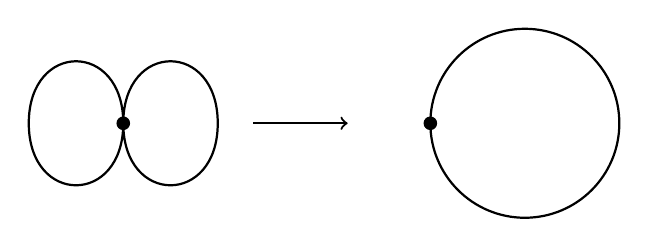
\begin{tikzpicture}[scale=1.5]
  
  % Figure 8 (left side)
  % Draw the two loops
 \draw[thick] (-1.4,0) .. controls (-1.4,0.7) and (-2.2,0.7) .. (-2.2,0)
               .. controls (-2.2,-0.7) and (-1.4,-0.7) .. (-1.4,0)
               .. controls (-1.4,0.7) and (-0.6,0.7) .. (-0.6,0)
               .. controls (-0.6,-0.7) and (-1.4,-0.7) .. (-1.4,0);
  
  % Mark the basepoint p on figure 8
  \filldraw (-1.4,0) circle (1.5pt);
  
  % Arrow pointing right
  \draw[->,thick] (-0.3,0) -- (0.5,0);
  
  % Circle (right side)
  \draw[thick] (2,0) circle (0.8);
  
  % Mark the basepoint p on circle
  \filldraw (1.2,0) circle (1.5pt);
  
\end{tikzpicture}
\end{center}
\begin{proof}
  Chose a Riemannian metric on $M$. Then, $f$ corresponds to a vector field $X_{df}$, where
  \begin{align*}
    g\left( X_{df},Y \right) &= df\left( Y \right)\\
                             &= Y(f).
  \end{align*}
  If $c\colon \R\rightarrow M$ is any curve, then we have that
  \begin{align*}
    g\left( \pd{c}{t},\nabla f \right) &= df\left( \pd{c}{t} \right).
  \end{align*}
  Let $\rho\colon M\rightarrow \R$ be defined by
  \begin{align*}
    \rho\left( p \right) &= \frac{1}{g\left( \nabla f,\nabla f \right)_{p}}
  \end{align*}
  on $f^{-1}\left( \left[ a,b \right] \right)$ and $0$ outside a small compact neighborhood of $f^{-1}\left( \left[ a,b \right] \right)$. We observe that $\rho$ is well-defined since $ \nabla f $ is nonzero on $f^{-1}\left( \left[ a,b \right] \right)$.%\newline

  Define a vector field $X$ by taking $X_{q} = \rho\left( q \right)\nabla f$, and let $\varphi_t$ be the flow generated by $X$. This flow is defined for all $t\in \R$ as $M$ is compact. If $q\in M$ is arbitrary, then the map $t\mapsto f\left( \varphi_t(q) \right)$ takes $\R\rightarrow \R$. In particular, if $q\in f^{-1}\left( \left[ a,b \right] \right)$, then
  \begin{align*}
    \iprod{\pd{}{t}\varphi_t(q)}{\nabla f} &\coloneq \iprod{X}{\nabla f}\\
                                           &= 1
  \end{align*}
  by the definition of $X$. Therefore, we have that the map is linear with derivative $1$. In particular, we can observe that $\varphi_{b-a}$ is a map from $M^{b}$ to $M^{a}$, and is thus a diffeomorphism.
\end{proof}
Next, to build the CW decomposition of $M$, we examine singular critical point.
\begin{theorem}
  Let $c\in \R$ be a critical value for a Morse function $f\colon M\rightarrow \R$. Furthermore, assume that $f^{-1}\left( \set{c} \right)$ has no critical points. Then,
  \begin{align*}
    M^{c+\ve} &\simeq M^{c-\ve}\bigcup_{\partial e^{\lambda}}e^{\lambda}
  \end{align*}
  are homotopy equivalent. Here, $e^{\lambda}$ denotes the closed ball in $\R^{\lambda}$, which is known as a \textit{$\lambda$-cell}.
\end{theorem}
\begin{proof}
  Choose coordinates about $p$ such that
  \begin{align*}
    f &= c-u_1^2-\cdots-u_{\lambda}^2 + u_{\lambda+1}^2 + \cdots + u_n^2.
  \end{align*}
  Choose $\ve > 0$ such that $f^{-1}\left( \left[ c-\ve,c+\ve \right] \right)$ contains exactly one critical point. Assume that the image $U$ of $\left( u_1,\dots,u_n \right)$ contains a closed ball with radius $\sqrt{2}\ve$. Let
  \begin{align*}
    e^{\lambda} &= \set{\left( u_1,\dots,u_{\lambda},0,\dots,0 \right) | u_1^2 + \cdots + u_{\lambda}^2\leq \ve}.
  \end{align*}
  In particular, we will show that $M^{c+\ve}$ deformation retracts to $M^{c-\ve}\cup e^{\lambda}$.%\newline

  Let $\mu\colon \R\rightarrow \R$ be smooth such that $\mu\left( 0 \right) > \ve$ and $u(r) = 0$ for $r\geq 2\ve$. Then, we observe that
  \begin{align*}
    -1 < \pd{\mu}{r} \leq 0.
  \end{align*}
  Set
  \begin{align*}
    F &= f - \mu\left( u_1^2 + \cdots + u_{\lambda}^2 + u_{\lambda +1}^2 + \cdots + u_n^2 \right).
  \end{align*}
  Observe that $F$ is a globally defined function on $M$ with $F = f$ outside the chart for $p$. We set
  \begin{align*}
    \xi &= u_1^2 + \cdots + u_{\lambda}^2\\
    \eta &= u_{\lambda + 1}^2 + \cdots + u_n^2.
  \end{align*}
  Then, we have
  \begin{align*}
    F &= c - \xi + \eta - \mu\left( \xi + 2\eta \right).
  \end{align*}
  We start by seeing that $F^{-1}\left( \left( -\infty,c+\ve \right] \right) = M^{c+\ve}$. This follows from the fact that $f$ and $F$ coincide outside $\xi + 2\eta \leq 2\ve$, while $F\leq f\leq c + \ve$ inside the ellipsoid.%\newline

  Additionally, the critical points of $F$ and $f$ agree, since
  \begin{align*}
    \pd{F}{\xi} &= -1-\mu'\left( \xi + 2\eta \right)\\
                &< 0\\
    \pd{f}{\eta} &= 1-2\mu'\left( \xi + 2\eta \right)\\
                 &> 1.
  \end{align*}
  We observe that
  \begin{align*}
    dF &= \pd{F}{\xi}d\xi + \pd{F}{\eta}d\eta
  \end{align*}
  is such that $dF = 0$ if and only if $d\xi$ and $d\eta = 0$, hence the ``origin'' (i.e., $p$) is the only critical point of $F$.%\newline

  Furthermore, since $F^{-1}\left( \left[ c-\ve,c+\ve \right] \right)\leq f^{-1}\left( \left[ c-\ve,c+\ve \right] \right)$, and
  \begin{align*}
    F(p) &= c-\mu(0)\\
         &< c-\ve,
  \end{align*}
  we have that $F(p) \notin \left[ c-\ve,c+\ve \right]$, whence $F^{-1}\left( \left( -\infty,c-\ve \right] \right)$ is a deformation retract of $M^{c+\ve}$.
  \begin{align*}
    F^{-1}\left( \left( -\infty,c-\ve \right] \right) &= M^{c-\ve} \cup H,
  \end{align*}
  where
  \begin{align*}
    H &= \overline{F^{-1}\left( \left( -\infty,c-\ve \right] \right)\setminus M^{c-\ve}}
  \end{align*}
  We have $e^{\lambda}\subseteq H$. We may define the deformation retract from $M^{c-\ve}\cup H$ to $M^{c-\ve}\cup e^{\lambda}$ via the following cases.
  \begin{enumerate}[(i)]
    \item If $\xi \leq \ve$, then
      \begin{align*}
        r_t &= \left( u_1,\dots,u_{\lambda},tu_{\lambda+1},\dots,tu_n \right).
      \end{align*}
      This maps $F^{-1}\left( \left( -\infty,c-\ve \right] \right)$ into itself, as $ \pd{F}{\eta} > 0 $, $r_1 = \id$, and $r_0 = e^{\lambda}$, with $r_t$ mapping the region $U$ into itself.
    \item If $\ve \leq \xi \leq \eta + \ve$, then we may define
      \begin{align*}
        r_t &= \left( u_1,\dots,u_{\lambda},s_tu_{\lambda+1},\dots,s_tu_{n} \right),
      \end{align*}
      where
      \begin{align*}
        s_t &= t + \left( 1-t \right)\left( \frac{\xi - \ve}{\eta} \right)^{1/2}.
      \end{align*}
    \item If $\eta + \ve \leq \xi$, then we may simply define $r_t = \id$.
  \end{enumerate}
\end{proof}
Now, we go on a little bit of a digression on CW complexes. We say a topological space $X$ is a (finite) CW complex if
\begin{align*}
  X &= \bigcup_{i=0}^{n} X^{(i)}.
\end{align*}
We call each $X^{(i)}$ the \textit{$i$-skeleton}, where
\begin{align*}
  X^{(0)} &= \set{p_1,\dots,p_n},
\end{align*}
and $X^{(i+1)}$ is given by attaching finitely many $\left( i+1 \right)$-balls, denoted $e^{i+1}$, to $X^{(i)}$ via maps $\psi\colon \partial e^{i+1}\rightarrow X^{(i)}$ that satisfy certain properties. An important fact about CW complexes is that if $\varphi\colon e^{\lambda}\rightarrow X$ is a map into a CW complex, and $f\colon X\rightarrow Y$ is a continuous map of topological spaces, then $f$ extends to a map $ \overline{f}\colon X\cup_{\varphi} e^{\lambda} \rightarrow Y\cup_{f\circ\varphi}e^{\lambda}$.
\begin{theorem}
  Every smooth manifold has the homotopy type of a CW complex.
\end{theorem}
\begin{proof}
  Let $c_1,\dots,c_n$ be the critical values of a (closed) manifold $M$. Then, $M^{a}$ is empty for $a < c_1$.%\newline

  If $c$ is a critical value of $f$, then
  \begin{align*}
    M^{c+\ve} &\simeq M^{c-\ve}\bigcup_{\varphi_1}e^{\lambda_1}\bigcup\cdots\bigcup_{\varphi_k}e^{\lambda_k}.
  \end{align*}
  By induction, $M^{c-\ve}$ is homotopy equivalent to some CW complex $K$. Therefore, from the fact above, it follows that
  \begin{align*}
    M^{c+\ve} &\simeq K\bigcup_{\varphi_1}e^{\lambda_1}\bigcup\cdots\bigcup_{\varphi_k}e^{\lambda_k}.
  \end{align*}
\end{proof}
\subsection{Some Applications of Morse Theory}%
Now that we have established that Morse functions (really, just one Morse function) allow(s) us to understand the global structure of a manifold, there are a variety of applications.
\begin{theorem}[Reeb's Sphere Theorem]
  If $M$ is closed, and there is some Morse function $f\colon M\rightarrow \R$ with exactly two critical points, then $M\cong S^n$ are homeomorphic.
\end{theorem}
The proof can be found \href{https://ncatlab.org/nlab/show/Reeb+sphere+theorem}{here}. Note that $M$ and $S^{n}$ are not diffeomorphic in the general case. Milnor (1956) established \href{https://webhomes.maths.ed.ac.uk/~v1ranick/papers/exotic.pdf}{the existence} of an exotic smooth structure on the $7$-sphere that is homeomorphic but not diffeomorphic to $S^{7}$ with the standard structure emerging from stereographic projections.%\newline

Our next application is understanding the de Rham cohomology of complex projective space $ \mathbb{CP}^n $. The cohomology of real projective space could be found by using invariant cohomology of $\Z/2\Z$ acting on $S^n$ via the antipodal map (or orientability of the space $ \mathbb{RP}^n $), and is given by
\begin{align*}
  H^{\ast}_{\operatorname{DR}}\left( \mathbb{RP}^n \right) &= \begin{cases}
    \R & k = 0\\
    0 & 1\leq k \leq n-1\\
    0 & k=n,n\text{ even}\\
    \R & k=n,n\text{ odd}
  \end{cases}.
\end{align*}
Unfortunately, $ \mathbb{CP}^n $ is a bit more complicated. Similar to real projective space, complex projective space $ \mathbb{CP}^n $ is given by ``lines'' in $\C^{n+1}$, where we view ``lines'' as complex lines. In other words, elements of $ \mathbb{CP}^n $ look like equivalence classes of homogeneous coordinates $ \left[ z_0:\cdots:z_n \right] $, where two classes
\begin{align*}
  \left[ z_0:\cdots:z_n \right] &= \left[ w_0:\cdots:w_n \right]
\end{align*}
if there is $\lambda\in \C$ with $w_i = \lambda z_i$ for all $i$. In particular, this means that we can restrict our view to representatives with Euclidean norm $1$. That is, elements $\left( z_0,\dots,z_n \right)$ with
\begin{align*}
  \sum_{i=0}^{n} \left\vert z_i \right\vert^2 &= 1.
\end{align*}
Standard charts for $ \mathbb{CP}^n $ are given by
\begin{align*}
  \varphi_i\colon \set{\left[ z_0:\cdots:z_n \right] | z_i\neq 0}\eqcolon V_i &\rightarrow \C^{n}\\
  \left[ z_0:\cdots:z_n \right] &\mapsto\left( \frac{z_0}{z_i},\dots,\frac{z_n}{z_i} \right),
\end{align*}
excluding $z_i$ itself. Note here that the origin is given by the equivalence class of $\left( 0,\dots,1,\dots,0 \right)$, where $1$ is in position $i$.%\newline

Now, let $c_0,\dots,c_n$ be distinct nonzero real numbers. Define the Morse function $f\colon \mathbb{CP}^n\rightarrow \R$ by
\begin{align*}
  f\left( \left[ z_0:\cdots:z_n \right] \right) &= \sum_{i=0}^{n}c_i \left\vert z_i \right\vert^2.
\end{align*}
This function is well-defined since any two representatives in our restricted view of $ \mathbb{CP}^n $ will differ by a multiple $\lambda$ with $\left\vert \lambda \right\vert = 1$.%\newline

We start with the chart $V_0$. Writing $\left( x_1,y_1 \right),\dots,\left( x_n,y_n \right)$ for the coordinates with $z_j = x_j + y_j$, we have that
\begin{align*}
  \left\vert z_0 \right\vert^2 &= 1-\sum_{j=1}^{n} \left( x_j^2 + y_j^2 \right),
\end{align*}
meaning that in the chart $V_0$, we have
\begin{align*}
  f &= c_0 + \sum_{j=1}^{n} \left( c_j-c_0 \right) \left( x_j^2 + y_j^2 \right).
\end{align*}
This is clearly a Morse function since we've already put it in the form that emerges from the Morse Lemma, and the only critical point of $f$ is the origin, as
\begin{align*}
  df &= \sum_{j=1}^{n}2\left( c_j-c_0 \right)x_j\:dx_j + \sum_{j=1}^{n}2\left( c_j-c_0 \right)y_j\:dy_j
\end{align*}
only equals zero at the origin since we have specified the $c_j$ to be distinct. This has an index given by $2$ times the number of $c_j$ with $c_j < c_0$. The corresponding point is $P_0 = \left( 1,0,\dots,0 \right)$.%\newline

Playing the same game with the charts centered at each of the $P_i$, we may march through all the critical points and observe that $f$ is Morse with exactly $n+1$ critical points, each of which has index $0,2,4,\dots,2n$. Thus,
\begin{align*}
  \mathbb{CP}^n &\simeq e^0\cup e^2\cup\cdots\cup e^{2n}.
\end{align*}
We write our chain complex below, where we let $C_n\left( X;\R \right)$ denote the free $\R$-vector space on $n$-cells in our CW decomposition.
\begin{center}
  % https://tikzcd.yichuanshen.de/#N4Igdg9gJgpgziAXAbVABwnAlgFyxMJZABgBpiBdUkANwEMAbAVxiRAB12BjKCHBAL6l0mXPkIoAjOSq1GLNgGEA+sDACAFAA0A3JwBKAShBCR2PASIAmGdXrNWiECrUBaSZt0HjpkBnPiRADMtnIObJw8fIKyMFAA5vBEoABmAE4QALZIZCA4EEgewiDpWYXU+Ug2YQpOnGh0aXiMJsWl2YjVlYhBAhQCQA
    \begin{tikzcd}
    \cdots \arrow[r] & C_{n}(X;\R) \arrow[r, "\partial"] & C_{n-1}(X;\R) \arrow[r] & \cdots
    \end{tikzcd}
\end{center}
As a result, we have that $C_i\left( \mathbb{CP}^n \right)\cong 0$ whenever $i$ is odd, so that
\begin{align*}
  H_{\ast}\left( \mathbb{CP}^n;\R \right) &= \begin{cases}
    \R & 0\leq k \leq 2n,k\text{ even}\\
    0 & \text{else}.
  \end{cases}
\end{align*}
\subsection{Existence of Morse Functions}%
Showing the existence of Morse functions will entail a tour of classical differential geometry. We let $M$ be a smooth $k$-manifold embedded into $\R^{n}$ with $n > k$. If $p\in \R^{n}$, define $L_p\colon M\rightarrow \R$ by
\begin{align*}
  L_p\left( q \right) &= \norm{p-q}^2,
\end{align*}
where $\norm{\cdot}$ is the norm on $\R^{n}$ induced from the standard Euclidean inner product, which we denote $ \iprod{\cdot}{\cdot} $. We will show the following theorem.
\begin{theorem}
  For almost every $p\in \R^{n}$, $L_p$ is Morse.
\end{theorem}
\begin{definition}
  If $M\hookrightarrow \R^{n}$ is embedded, then we define the \textit{normal space} of $p$ in $\R^{n}$ to be
  \begin{align*}
    N_pM &= \set{v\in \R^{n} | \iprod{v}{w} = 0\text{ for all }w\in T_pM}.
  \end{align*}
  The \textit{normal bundle} of $M$ in $\R^{n}$ is the space
  \begin{align*}
    NM &= \set{\left( q,v \right)\in \R^{n}\times \R^{n} | q\in M, v\in N_qM}.
  \end{align*}
  Observe that, similar to the tangent bundle, the normal bundle is a smooth submanifold of $\R^{2n}$.
\end{definition}
Given $\left( q,v \right)\in NM$, we define the \textit{endpoint map} $E\colon NM\rightarrow \R^{n}$ by $\left( q,v \right)\mapsto q+v$. 
\begin{definition}
  We call $e\in \R^{n}$ a \textit{focal point} for $\left( M,q \right)$ with multiplicity $a$ if $e = q + v$ for some $\left( q,v \right)\in NM$, and the matrix $J_{(q,v)}E$ is singular with nullity $a$.
\end{definition}
Note that by Sard's Theorem, almost every $x\in \R^{n}$ is \textit{not} a focal point.%\newline

To understand a little more about focal points, we discuss the first and second fundamental forms from classical differential geometry. Fix local coordinates $\left( u_1,\dots,u_k \right)$ on $M$, where we endow $\R^{n}$ with the standard coordinates $\left( x_1,\dots,x_n \right)$. We may write $x_i = x_i\left( u_1,\dots,u_k \right)$ for all $i = 1,\dots,n$. We call the matrix
\begin{align*}
  \left( \gamma_{ij} \right)_{i,j} &= \left( \iprod{\pd{x}{u_i}}{\pd{x}{u_j}} \right)_{i,j},
\end{align*}
where $x = \left( x_1,\dots,x_n \right)$, the \textit{first fundamental form} on $M$. It effectively reflects the Riemannian metric on $M$ inherited from $\R^{n}$. In particular, we may choose coordinates $\left( u_1,\dots,u_k \right)$ for $M$ such that $\left( \gamma_{ij} \right)_{i,j}$ is the identity matrix, as follows from the inverse function theorem applied to a change of coordinates matrix.%\newline

The next question that arises is how to relate the curvature of $M$. At each $q\in M$, we may compare the expression $ \pd{^2x}{u_i\partial u_j} $ to its normal component. The matrix of normal components,
\begin{align*}
  \left( \ell_{ij} \right)_{i,j} &= \left( \left( \pd{^2x}{u_i\partial u_j} \right)_{\perp} \right)_{i,j},
\end{align*}
is known as the \textit{second fundamental form}. Note that this is a $k\times k$ matrix of vectors in $\R^{n}$. If $v\in \R^{n}$, then we consider the real-valued matrix $\left( \left\langle v, \ell_{ij} \right\rangle \right)_{i,j}$. From Clairaut's Theorem, this matrix is diagonalizable with $k$ eigenvalues, denoted $\kappa_{1,v},\dots,\kappa_{k,v}$. We call these eigenvalues the \textit{principal curvatures} of $M$ at $q$ in the direction $v$. The values $\rho_{i,v} = \frac{1}{\kappa_{i,v}}$ are known as the \textit{principal radii of curvature}.
\begin{proposition}
  The focal points of $M$ at $q$ are precisely the points $q + \rho_i v$ for any unit vector $v\in N_qM$.
\end{proposition}
\begin{proof}
  Fix pairwise orthogonal locally defined vector fields $w_1,\dots,w_{n-k}$ that span $N_qM$. Letting $x_i = x_i\left( u_1,\dots,u_k \right)$ be coordinates on $M$ defined such that $\left( \gamma_{ij} \right)_{i,j} = \id$. We have that
  \begin{align*}
    e\left( u_1,\dots,u_k,t_1,\dots,t_{n-k} \right) &= x + \sum_{\alpha=1}^{n-k}t_{\alpha}w_{\alpha}
  \end{align*}
  is our endpoint map. We have
  \begin{align*}
    \pd{e}{u_i} &= \pd{x}{u_i} + \sum_{\alpha = 1}^{n-k}t_{\alpha}\pd{w_{\alpha}}{u_i}\\
    \pd{e}{t_{\beta}} &= w_{\beta}.
  \end{align*}
  Taking inner products between $e$ and the coordinate vectors
  \begin{align*}
    \left( x,w \right) &= \left( \pd{x}{u_1},\dots,\pd{x}{u_k},w_1,\dots,w_{n-k} \right),
  \end{align*}
  we have the block-diagonal matrix
  \begin{align*}
    A &= \begin{pmatrix}\left( \iprod{\pd{x}{u_i}}{\pd{x}{u_j}} + \sum_{\alpha=1}^{n-k}t_{\alpha}\pd{w_{\alpha}}{u_i}\pd{x}{u_j} \right)_{i,j} & \left( \sum_{\alpha=1}^{n-k}t_{\alpha} \iprod{\pd{w_{\alpha}}{u_i}}{w_{\beta}} \right)\\0 & I\end{pmatrix},
  \end{align*}
  and if we let $K$ be the first block, then we have that $\dim\left( \ker\left( A \right) \right) = \dim\left( \ker\left( K \right) \right)$. The first term in $K$ is
  \begin{align*}
    \left( \iprod{\pd{x}{u_i}}{\pd{x}{u_j}} \right)_{i,j} &= \left( \gamma_{ij} \right)_{i,j},
  \end{align*}
  which is the first fundamental form. In particular, we also have
  \begin{align*}
    0 &= \iprod{w_{\alpha}}{ \pd{x}{u_j} }\\
      &= \pd{}{u_i} \left( \iprod{w_{\alpha}}{ \pd{x}{u_j} } \right)\\
      &= \iprod{\pd{w_{\alpha}}{u_i}}{\pd{x}{u_j}} + \iprod{w_{\alpha}}{ \pd{^2x}{u_i\partial u_j} }\\
      &= \iprod{\pd{w_{\alpha}}{u_i}}{\pd{x}{u_j}} + \iprod{w_{\alpha}}{\ell_{ij}}.
  \end{align*}
  Thus,
  \begin{align*}
    K &= \left( \gamma_{ij} - \sum_{\alpha=1}^{n-k}t_{\alpha} \iprod{w_{\alpha}}{\ell_{ij}} \right)_{i,j}.
  \end{align*}
  In particular, $J_{(q,v)}(E)$ has nullity $\mu$ if and only if
  \begin{align*}
    \left( \gamma_{ij} - \sum_{\alpha=1}^{n-k}t_{\alpha} \iprod{w_{\alpha}}{\ell_{ij}} \right)_{i,j} &= \left( I_k-\sum_{\alpha=1}^{n-k}t_{\alpha} \iprod{w_{\alpha}}{\ell_{ij}} \right)_{i,j}
  \end{align*}
  has nullity $\mu$. Considering the line $\ell = q + tv$ for $v\in N_qM$, we find that this is equal to $\left( I_k - t \left\langle v, \ell_{ij} \right\rangle \right)_{i,j}$, which is singular if and only if $\left( \frac{1}{t}I_k- \left\langle v, \ell_{ij} \right\rangle \right)_{i,j}$ is singular, whence $\frac{1}{t}$ is a principal curvature of $M$ at $q$ in the direction of $v$.
\end{proof}
We will use this as part of our proof of the main theorem.
\begin{theorem}
  For almost every $p\in \R^{n}$, the function
  \begin{align*}
    L_p(x) &\eqcolon f(x)\\
           &= \norm{x-p}^2\\
         &= \iprod{x}{x} - 2 \iprod{x}{p} + \iprod{p}{p}
  \end{align*}
  is Morse.
\end{theorem}
\begin{proof}
  Computing directly, we find that
  \begin{align*}
    \pd{f}{u_i} &= 2 \iprod{\pd{x}{u_i}}{x} - 2 \iprod{\pd{x}{u_i}}{p}\\
                &= 2 \iprod{\pd{x}{u_i}}{x-p}.
  \end{align*}
  Therefore, $f$ has a critical point at $q$ if and only if $df = 0$, meaning that $\pd{f}{u_i} = 0$ for all $u_i$ meaning that $q-p$ is a normal vector for $M$.%\newline

  Next, we compute
  \begin{align*}
    \pd{^2f}{u_i\partial u_j} &= 2 \left( \iprod{\pd{x}{u_i}}{\pd{x}{u_j}} + \iprod{\pd{^2x}{u_i\partial u_j}}{x-p} \right).
  \end{align*}
  Setting $p = x + tv$ for some $v$ normal to $M$ at $x$, we have
  \begin{align*}
    \pd{^2f}{u_i\partial u_j} &= 2 \left( \iprod{\pd{x}{u_i}}{\pd{x}{u_j}} - t \iprod{v}{\ell_{ij}} \right)\\
                              &= 2 \left( \gamma_{ij} - t \iprod{v}{\ell_{ij}} \right).
  \end{align*}
  Therefore, if $q$ is a critical point for $f$, then $q$ is degenerate if and only if $p$ is a focal point for $M$ at $q$.

  By Sard's Theorem, this implies that for almost every $p\in \R^{n}$, $L_p$ is Morse.
\end{proof}
\section{Notations}%
\begin{itemize}
  \item A general normed space $V$ will have its norm denoted by $\norm{\cdot}$. If $V = \R^{n}$, then we denote the norm by $ \left\vert \cdot \right\vert $.
  \item We denote topological spaces by $\left( X,\tau \right)$.
  \item $ U\left( x,r \right) = \set{y\in V | \norm{x-y} < r}$.
  \item $ B\left( x,r \right) = \set{y\in V | \norm{x-y} \leq r}$.
  \item $ \mathcal{N}_p $: neighborhood system centered at $p\in X$.
  \item $ \mathcal{O}_p $: system of \textit{open} neighborhoods centered at $p\in X$.
  \item When we say a number $n$ is positive, we mean that $n\geq 0$. Similarly, a sequence $\left( a_n \right)_n$ is decreasing (increasing) if $a_n\geq a_{n+1}$ ($a_n\leq a_{n+1}$).
  \item We define $\mathcal{C}_{p,M}$ to be the space of $C^{\infty}$ functions $\varphi\colon \left( -\ve,\ve \right)\rightarrow M$ such that $\varphi(0) = p$.
  \item We write $\mathcal{X}\left( M \right)$ to be the space of vector fields on $M$.
\end{itemize}
\end{document}
